%\documentclass[11pt,a4paper,oneside]{book}
%\usepackage[hmargin={1.25in,1.25in},vmargin={1.25in,1.25in}]{geometry}




\documentclass[12pt,a4paper,oneside]{book}
\usepackage{setspace}
\onehalfspacing
\usepackage[hmargin={3.5cm,1.5cm},vmargin={2.5cm,2.5cm}]{geometry}


\usepackage[french]{babel}
\usepackage[utf8]{inputenc}
\usepackage[T1]{fontenc}

\usepackage{graphicx}

\usepackage[final]{pdfpages} % include pdf files

\usepackage[colorinlistoftodos]{todonotes}
\usepackage{amsthm}
\usepackage{amsmath}
\usepackage{amsfonts}
\usepackage{tabularx}
%\usepackage[nottoc, notlof, notlot]{tocbibind}
\usepackage{charter}

\usepackage{url}
%\usepackage{geometry}
\usepackage{enumitem}
\usepackage{hyperref}
\usepackage{comment}
\usepackage{listings} 
\usepackage{caption} 
\usepackage{stmaryrd}

\newcounter{nalg}[chapter] % defines algorithm counter for chapter-level
\renewcommand{\thenalg}{\thechapter .\arabic{nalg}} %defines appearance of the algorithm counter
\DeclareCaptionLabelFormat{algocaption}{Algorithm \thenalg} % defines a new caption label as Algorithm x.y


\lstnewenvironment{algorithm}[1][] %defines the algorithm listing environment
{   
    \refstepcounter{nalg} %increments algorithm number
    \captionsetup{labelformat=algocaption,labelsep=colon} %defines the caption setup for: it ises label format as the declared caption label above and makes label and caption text to be separated by a ':'
    \lstset{ %this is the stype
        frame=tB,
        numbers=left, 
        numberstyle=\tiny,
        basicstyle=\scriptsize, 
        keywordstyle=\color{black}\bfseries\em,
        keywords={,input, output, return, then, endif, datatype, function, in, if, else, foreach, while, begin, end, } %add the keywords you want, or load a language as Rubens explains in his comment above.
        numbers=left,
        xleftmargin=.04\textwidth,
        #1 % this is to add specific settings to an usage of this environment (for instnce, the caption and referable label)
    }
}
{}




\graphicspath{{graphes/}}



\newtheoremstyle{break}  % follow `plain` defaults but change HEADSPACE.
  {\topsep}   % ABOVESPACE
  {\topsep}   % BELOWSPACE
  {}  % BODYFONT
  {0pt}       % INDENT (empty value is the same as 0pt)
  {\bfseries} % HEADFONT
  {.}         % HEADPUNCT
  {\newline}  % HEADSPACE. `plain` default: {5pt plus 1pt minus 1pt}
  {}          % CUSTOM-HEAD-SPEC
\theoremstyle{break}

\newtheorem{defin}{Définition}[chapter]
\def\definautorefname{Définition}
\newtheorem{exem}{Exemple}[chapter]
\def\exemautorefname{Exemple}




\newtheoremstyle{breakplain}  % follow `plain` defaults but change HEADSPACE.
  {\topsep}   % ABOVESPACE
  {\topsep}   % BELOWSPACE
  {\itshape}  % BODYFONT
  {0pt}       % INDENT (empty value is the same as 0pt)
  {\bfseries} % HEADFONT
  {.}         % HEADPUNCT
  {\newline}  % HEADSPACE. `plain` default: {5pt plus 1pt minus 1pt}
  {}          % CUSTOM-HEAD-SPEC
\theoremstyle{breakplain}
\newtheorem{theo}{Théorème}[chapter]
\def\theoautorefname{Théorème}
\newtheorem{lem}{Lemme}[chapter]
\def\lemautorefname{Lemme}
\newtheorem{prop}{Proposition}[chapter]
\def\propautorefname{Proposition}

\title{Préparation au mémoire --- MEMO-F-403\\Ordonnancement de systèmes à criticité mixte et méthodes formelles}
\author{Simon \textsc{Picard}}
\date{22 mai 2015}

\begin{document}
%\maketitle
\begin{titlepage}
\begin{center}
\textbf{UNIVERSIT\'E LIBRE DE BRUXELLES}\\
\textbf{Faculté des Sciences}\\
\textbf{Département d'Informatique}
\vfill{}\vfill{}
%\begin{center}
{\Huge  Ordonnancement de systèmes à criticité mixte et méthodes formelles}
%\end{center}
{\Huge \par}
\begin{center}{\LARGE Simon \textsc{Picard}}\end{center}{\Huge \par}
%\vfill{}\vfill{}\vfill{}\vfill{}\vfill{}
\vfill{}

\includegraphics[width=\textwidth-2cm]{images/sceau-b-quadri.jpg}
\vfill{}
\begin{flushright}{\large \textbf{Promoteurs :}}\hfill{}{\large Mémoire présenté en vue de}\\
{\large Prof. Gilles Geeraerts}\hfill{}{\large l'obtention du grade de}\\{\large Prof. Joël Goossens}
\hfill{}{\large Master en Sciences Informatiques}\end{flushright}{\large\par}
\vfill{}\vfill{}\enlargethispage{2cm}
\textbf{Année académique 2015~-~2016}
\end{center}
\end{titlepage}

\newpage
\thispagestyle{empty} 
\null



\frontmatter



\chapter*{Abstract}

\chapter*{Résumé}

\chapter*{Remerciements}

\tableofcontents


\mainmatter


\chapter{Introduction}
Ce document a été réalisé dans le cadre du second cycle d'études à l'ULB en sciences informatiques. C'est la première partie du travail total que représente le mémoire. Le but est de se lancer dans la rédaction d'un travail de fin d'études porté sur un sujet choisi par l'étudiant, qui comprend en premier lieu un état de l'art et ensuite un travail personnel sur le sujet défini à la fin de ce papier. La partie état de l'art porte essentiellement sur la recherche bibliographique, la lecture et la compréhension. Ce travail est réalisé sous la direction des professeurs Gilles Geeraerts et Joël Goossens.


\chapter{État de l'art}

Ce chapitre présente l'état de l'art ayant pour sujet deux problèmes différents de deux domaines différents de l'informatique.\\
Premièrement, le chapitre se concentre sur l'ordonnancement à criticité mixte. Pour se faire, il faut commencer par introduire l'ordonnancement classique, puis une explication informelle de ce type d'ordonnancement est donnée pour enfin terminer par le formalisme de celui-ci.\\
Dans un second temps, le problème de l'accessibilité est présenté, en commençant par fournir certaines notions de base, ensuite en exposant un formalisme pour finir par expliquer la notion d'antichaîne. Par la suite, l'interaction entre ces deux problèmes est mise au clair.\\
Enfin, les contributions qui seront faites dans ce mémoire seront détaillées.

\section{Ordonnancement de systèmes à criticité mixte}
\subsection{Notions élémentaires}
L'un des domaines majeurs de l'informatique théorique actuelle est celui de l'ordonnancement. Il s'agit d'organiser dans le temps la réalisation de différents travaux, compte tenu de contraintes temporelles. Pour s'exécuter, ces travaux ont besoin d'avoir accès à une ou plusieurs ressources partagées entre eux. En pratique, une fois qu'un travail est généré, il possède un temps d'exécution et une échéance. Dans la plupart des cas, on parle de système comprenant une série de travaux, le but est alors d'agencer ces différents travaux de sorte qu'ils ne ratent pas leurs échéances, il faut partitionner la ou les ressources partagées entre les travaux. L'objet de cette sous-section est de définir un certain modèle pour ce problème ainsi que d'introduire différentes notions de la théorie de l'ordonnancement.
\subsubsection{Modèle}
Pour permettre l'ordonnancement d'un système, un certain formalisme a été défini, cette partie le présente.\\

Commençons par une notion fondamentale, le travail. Il s'agit d'un ensemble d'opérations à effectuer nécessitant de prendre possession de la ou d'une des ressources partagées.

\begin{defin}[Travail \cite{goossens2014os}]
Un travail est représenté par un triplet : 
\begin{center}
$J_i = (r_i, d_i, c_i)$
\end{center}
\begin{itemize}
\item $r_i \in \mathbb{N}^{+}$ est l'instant auquel $J_i$ est généré.
\item $d_i \in \mathbb{N}^{+}$ est l'échéance absolue de $J_i$, c'est-à-dire le moment avant lequel le travail doit impérativement avoir été exécuté complètement. On assume que $d_i > r_i$
\item $c_i \in \mathbb{N}^{+}$ définit la durée d'exécution du travail.
\end{itemize}
Le travail $J_i$ doit donc recevoir $c_i$ unités de processeur durant l'intervalle $[r_i, d_i)$. $[a,b)$ est l'intervalle entre $a$ et $b$, $a$ est inclus et $b$ ne l'est pas. \\
En général, on parle d'instance $I$, il s'agit d'un ensemble de travaux : $ I = \{J_1, J_2, ...\} $
\end{defin}

Souvent, le programme à exécuter possède une partie d'opération récurrente, en particulier on considère les tâches périodiques et sporadiques.

\begin{defin}[Tâche périodique \cite{goossens1999scheduling}]
Une tâche périodique génère donc un nombre infini de travaux, elle est représentée par un quadruple :
\begin{center}
$\tau_i = (O_i, T_i, D_i, C_i)$
\end{center}
\begin{itemize}
\item $O_i \in \mathbb{N}^{+}$ est le décalage de la tâche, l'instant auquel le premier travail de la tâche est généré.
\item $C_i \in \mathbb{N}^{+}$ définit la durée d'exécution d'un travail généré par la tâche.
\item $D_i \in \mathbb{N}^{+}$ est l'échéance relative de la tâche, c'est donc le laps de temps entre la génération d'un travail et son échéance absolue.
\item $T_i \in \mathbb{N}^{+}$ est la périodicité de la tâche, c'est-à-dire l'intervalle entre deux générations de travail.\\
\end{itemize}
Le $k^{e}$ travail $J_{i,k}$ de la tâche $\tau_i$ est donc généré à l'instant $O_i + (k-1)*T_i$ et a pour échéance  $O_i+(k-1)*T_i+D_i$ .
\end{defin}
\begin{defin}[Tâche sporadique \cite{goossens1999scheduling}]
Une tâche sporadique possède le même modèle que la tâche périodique, la différence est que $T_i$ ne représente plus la périodicité, mais le temps minimal entre deux générations de tâche. La tâche sporadique est donc imprévisible.
\end{defin}


On définit ensuite une série caractéristique \cite{goossens1999scheduling} qu'une tâche peut avoir :
\begin{itemize}
\item Une tâche à échéance implicite est une tâche où l'échéance correspond à la période, $D_i = T_i\ \forall i$
\item Une tâche à échéance contrainte est une tâche où l'échéance est inférieure ou égale à la période, $D_i \le T_i\ \forall i$
\item Une tâche à échéance arbitraire est une tâche où il n'y a pas de contraintes en la période et l'échéance de celle-ci.
\end{itemize}
On définit ensuite, sur un système de plusieurs tâches $\tau = \{\tau_1, \tau_2, ...\}$
\begin{itemize}
\item Un système de tâche est synchrone si toutes ses tâches ont un décalage nul, $O_i = 0\ \forall i$
\item Asynchrone sinon.\todo{expliquer}
\end{itemize}

\subsubsection{Ordonnancement}
Une stratégie d'ordonnancement est un algorithme permettant le partage d'une ou plusieurs ressources entre plusieurs parties dont elles font la requête de manière simultanée et asynchrone \cite{goossens2014os}. Les ordonnanceurs sont utilisés, par exemple, dans un système d'exploitation, dans les disques durs, dans les routeurs internet ... Le but d'un ordonnanceur classique est d'éviter le gaspillage de ressource et de partager cette dernière de manière équitable entre ceux qui le demandent. Dans un ordonnanceur temps réel, une contrainte de temps doit être respectée, il faut que les processus se terminent avant leurs échéances, ce type d'ordonnanceur est largement utilisé dans les systèmes embarqués, par exemple dans un cardiostimulateur.\\

À l'heure actuelle, les constructeurs de systèmes embarqués ont tendance à implémenter plusieurs fonctionnalités sur une même plateforme pour réduire les coûts, la chaleur, l'alimentation... Malheureusement, un tel partage de ressource peut mener à des interférences entre les différents clients, on cherche donc à savoir si un tel ensemble de clients peuvent partager une ressource sans qu'il y ait de moments où un client n'a pas accès à cette ressource alors qu'il en a besoin.\\

Typiquement, on parle d'ordonnancement d'un processeur, on divise donc le temps d'exécution disponible grâce aux coups d'horloge, définissant le temps entre deux coups d'horloge successifs comme une unité de temps. L'ordonnanceur peut être préemptif, c'est-à-dire qu'il peut interrompre un travail pour en ordonnancer un autre.\\

Dans ce document, nous nous concentrerons sur les algorithmes d'ordonnancement préemptif sur un monoprocesseur à vitesse unitaire.\\

L'algorithme d'ordonnancement devra choisir parmi plusieurs travaux lequel pourra jouir de la puissance du processeur.  Pour ce faire, il utilisera un système de priorité clair et défini, chaque travail possédera une priorité et, en fonction de laquelle, l'ordonnanceur pourra partager le temps de calcul entre les travaux. Il existe trois classes d'algorithme d'ordonnancement \cite{goossens2014os} :\\

\begin{itemize}
\item Priorité fixe au niveau des tâches (Fixed Task Priority, FTP) : il s'agit d'un ordonnancement où chaque tâche s'est vue attribuer une priorité avant l'exécution du système. Chaque travail hérite ensuite de la priorité de la tâche qui l'a générée.
\item Priorité fixe au niveau des travaux (Fixed Job Priority, FJP) : chaque travail reçoit un niveau de priorité lorsqu'il est généré, celui-ci restera constant pour toute la durée du travail. Dès lors, différents travaux d'une même tâche peuvent avoir une priorité différente.
\item Priorité dynamique (Unrestructed Dynamic Priority, DP) : il s'agit du cas général où aucune contrainte ne s'applique à l'assignation des priorités aux travaux. En règle générale, cette nouvelle ligne conduite signifie qu'un travail va changer de priorité durant son existence.\\
\end{itemize}
On remarque que ces différentes classifications s'incluent elles-mêmes, en effet, FTP fait partie de la classe FJP qui est elle-même dans la classe DP.\\

L'ordonnancement est donc avant tout une certaine assignation de priorité. De manière générale, on considère que la valeur de la priorité attribuée à un travail est un naturel et est inversement proportionnel à sa priorité. Si deux travaux ont une même priorité, il faudra choisir de manière déterminée lequel sera ordonnancé. On définit donc la relation de priorité par le symbole $\succ$, par exemple : $\tau_i \succ \tau_j$, ici $\tau_i$ a une priorité supérieure à celle de $\tau_j$.\\

\begin{defin}[Fonction de priorité \cite{santy2012ordonnancement}]
Formellement, une fonction de priorité $\pi$ assigne à toute tâche $\tau_i$ d'un système de $n$ tâches $\tau$ (respectivement à tout travail $J_i$ d'une instance de $m$ travaux $I$) un nombre entier $\pi(\tau_i)$ (respectivement $\pi(J_i)$) compris entre $1$ et $n$ (respectivement $m$) qui représente de manière inversement proportionnelle la priorité de la tâche (respectivement du travail).
\begin{center}
$\pi : \tau \rightarrow \{0,...,n \}$\\
(Respectivement $\pi : I \rightarrow \{0,...,m \}$)\\
$\pi(\tau_i) < \pi(\tau_j) \Leftrightarrow \tau_i \succ \tau_j$\\
(Respectivement $\pi(J_i) < \pi(J_j) \Leftrightarrow J_i \succ J_j$)
\end{center}
\end{defin}

En temps réel, l'ordonnancement se porte en général sur un système de tâche. On souhaite prouver si un tel ensemble remplit les conditions introduites par ce mode. Deux nouvelles caractéristiques en émergent \cite{goossens2014os} :

\begin{itemize}
\item La faisabilité d'un système de tâche est vérifiée s'il existe un certain partage du temps de calcul entre les différents travaux, de sorte que chacun d'entre eux ait pu exécuter toutes leurs actions sans rater leur échéance.
\item Un système de tâche est ordonnançable avec un certain algorithme d'ordonnancement si celui-ci permet d'agencer les travaux de sorte que chacun d'entre eux ait pu exécuter toutes leurs actions sans rater leur échéance.\\
\end{itemize}

Une définition analogue peut être faite pour une collection de travaux.\\

Il est à noter qu'il est possible dans certains cas qu'un système de tâche soit faisable, mais pas ordonnançable. Ces deux notions sont souvent liées à celle de l'utilisation qui représente la charge de travail du processeur : la quantité de travail effectué par rapport au temps dont il dispose pour le faire.

\begin{defin}[Utilisation \cite{goossens2014os}]
L'utilisation d'une tâche est définie par la fonction $U(\tau_i) = C_i/T_i$.\\
L'utilisation d'un système est la somme des utilisations des tâches le composant : $U(\tau) = \underset{\tau_i \in \tau}{\sum} (\tau_i)$
\end{defin}

Pour clôturer cette sous-section, un algorithme d'ordonnancement monoprocesseur est présenté. Il s'agit d'un algorithme à priorité statique au niveau des travaux (FJP) : EDF (Earliest Deadline First). Celui-ci attribue à chacun des travaux une priorité relative à leurs échéances absolues, plus elles sont proches, plus le travail est prioritaire. Formellement, on obtient $d_i < d_j \Leftrightarrow J_i \succ J_j$ et en cas d'égalité, $d_i = d_j \wedge i < j \Leftrightarrow J_i \succ J_j$.

\begin{theo}[\cite{goossens2014os}]
Si une collection de travaux est faisable, alors elle est ordonnançable avec EDF.
\end{theo}

EDF est donc un algorithme optimal pour un système de tâche à échéance implicite, synchrone ou asynchrone. Un algorithme est optimal si l'agencement qu'il génère permet d'ordonnancer tout système de tâche d'un certain type.

\begin{theo}[\cite{liu1973scheduling}]
Pour un système de tâche périodique à échéance implicite $\tau$, celui-ci est faisable si et seulement si $U(\tau) \leq 1$
\end{theo}

\begin{figure}[h]
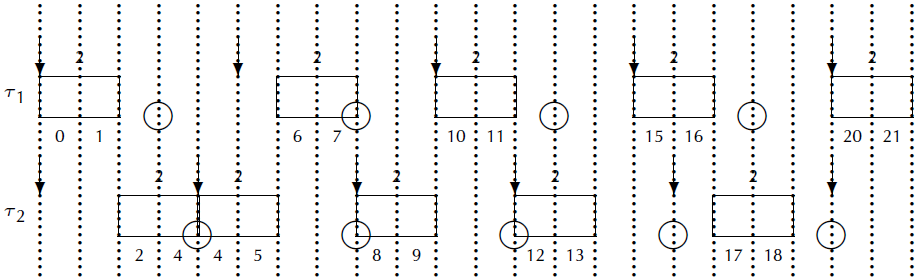
\includegraphics[width = \textwidth]{images/schedexample.png}
\caption{Représentation graphique d'un exemple d'ordonnancement par EDF \cite{goossens2014os}}
\label{edfsched}
\end{figure}

Il sera fréquent de représenter l'ordonnancement de travaux de manière graphique, la figure~\ref{edfsched} en est un exemple, ici il s'agit d'un système de deux tâches.
\begin{center}
$ \tau_1 = (0, 5, 3, 2) $\\
$ \tau_2 = (0, 4, 4, 2) $
\end{center}
Sur l'image :
\begin{itemize}
\item Chaque colonne en pointillé représente une unité de temps.
\item Une tâche est représentée sur une ligne
\item La flèche vers le bas représente la période de la tâche et donc le moment où le travail est généré
\item Un rond représente l'échéance d'un travail
\item Un carré représente l'exécution d'un travail durant une unité de temps
\end{itemize}

\subsection{Criticité mixte}
\subsubsection{Définition informelle}
Le problème de criticité mixte est un problème d'ordonnancement. Pour rappel, il s'agit donc de gérer le partage d'un ensemble de ressources communes entre plusieurs clients.\\

Dans cette sous-section, nous nous penchons sur un problème plus précis : celui de la certification, dont le but est de prouver qu'un système est ordonnançable.\\

Précédemment, il a été présenté l'ordonnancement de travaux classique, ici on en déduit un nouveau problème où les clients pourraient avoir une importance plus ou moins élevée en fonction de leur criticité dans leur système. 
Il est évident que, dans une voiture, le système de freins ABS (<<Anti-lock Brake System>>) est plus important, plus critique que l'autoradio, car, en cas de dysfonctionnement, il y a danger pour le conducteur, et donc l'ABS devrait être prioritaire sur l'autoradio, c'est-à-dire que si ces deux clients souhaitent prendre possession du processeur, mais que seul l'un des deux le peut, l'ABS sera privilégié. Ce problème d'ordonnancement avec différentes priorités est très actuel. En effet, c'est un domaine de recherche croissant dans le monde de l'ordonnancement temps réel et des systèmes embarqués, il fait l'objet d'un programme au sein du laboratoire <<US Air Force Laboratory>>, le Mixed-Criticality Architecture Requirements (MCAR) \cite{de2009scheduling}.\\

Dans le milieu aérospatial, le problème a été standardisé par l'organisme RTCA, qui classifie les travaux en fonction de la gravité qu'engendrerait un dépassement de leur échéance, il s'agit du standard DO-178C imprimé en figure~\ref{do178}.\\
\begin{figure}[h]
\begin{tabularx}{\textwidth}{|c|c|X|}
\hline
Niveau & Gravité & Conséquences\\
\hline
A & Catastrophique & Un échec peut causer multiple décès, habituellement avec la perte de l'objet volant\\
\hline
B & Hasardeuse & Un échec a un grand impact négatif sur la sûreté ou la performance, ou réduit la capacité de l'équipage à gérer l'objet volant à cause de détresse physique ou d'une charge de travail plus importante ou bien engendre de sérieuses blessures parmi les passagers.\\
\hline
C & Majeure & Un échec réduit significativement la marge de sûreté ou augmente significativement le travail de l'équipage. Par exemple, il pourrait engendrer un inconfort pour un passager (voire même une blessure).\\
\hline
D & Mineure & Un échec réduit légèrement la marge de sûreté ou augmente légèrement le travail de l'équipage. Par exemple, il pourrait engendrer un désagrément pour un passager dont le personnel devrait s'occuper.\\
\hline
E & Sans effet & Un échec n'a pas d'impact sur la sûreté, les opérations d'aviation ou la répartition du travail du personnel\\
\hline
\end{tabularx}
\caption{Standard RTCA DO-178C \cite{nordhoff2012do178}}
\label{do178}
\end{figure}

L'objectif de l'ordonnancement serait alors de permettre aux tâches les plus critiques de ne pas souffrir de perte de performance en cas de diminution des ressources, cette facette du problème a permis d'introduire la notion de criticité, mais ne sera pas traité dans ce mémoire.\\

Il existe un second aspect de l'ordonnancement à criticité mixte où un système devrait être garanti fonctionnel à plusieurs niveaux \cite{barhorst2009research}. Pour illustrer ce concept, nous utiliserons l'exemple des drones, UAV (unmmaned aerial vehicle), de reconnaissance. Nous distinguons deux niveaux de criticité dans ce type de système

\begin{itemize}
\item Criticité au vol : ce sont les actions exécutées par le drone pour voler en tant que tel, calculer un chemin pour éviter les obstacles, gérer la puissance des réacteurs, l'inclinaison des ailes ...
\item Criticité à la mission : ce sont toutes les actions qui fonctionnent dans le but de mener à bien la mission du drone. Dans notre cas, elles pourraient être le fait de filmer avec une caméra, de transmettre ces images ou d'autres informations, telles que la température extérieure, de faire de la reconnaissance sur ces images etc.\\
\end{itemize}

Il est évident que le niveau critique de vol est plus important que celui de la mission. En effet, si une des actions en rapport avec le vol du drone dysfonctionnait, cette défaillance pourrait mener à un atterrissage forcé qui entraînerait des dégâts matériels, voire même pire, un réel danger pour un être humain.\\

Pour introduire les contraintes sur les fonctionnalités, nous introduisons la notion de WCET (Worst-Case Execution Time), qui représente le temps d'exécution dont aura besoin une action pour s'exécuter complètement au pire des cas. Ces estimations sont très importantes, puisque tout le système d'ordonnancement repose sur elles. En effet, si un travail prend plus de temps à s'exécuter que l'estimation, le système complet peut être compromis. L'estimation du WCET doit être \cite{santy2012ordonnancement} :

\begin{itemize}
\item sûre. La validité d'une certification repose sur cette valeur, elle doit donc former une borne supérieure la plus juste possible. Il est exclu que celle-ci soit vue à la baisse, elle ne peut être optimiste.
\item la moins pessimiste possible. Plus le WCET est pessimiste, plus il induira des instants oisifs durant l'ordonnancement puisqu'en pratique, le temps d'exécution sera fréquemment inférieur à celui-ci. L'estimation ne doit pas être surestimée, sous peine d'engendrer un faux négatif lors d'un test d'ordonnançabilité.\\
\end{itemize}

Le calcul d'un WCET sûr et non pessimiste est un exercice difficile et n'est pas à prendre à la légère. Il s'agit d'un domaine à part entière des sciences informatiques, actuellement en plein essor qui fait l'objet de divers concours.\\

Comme en témoigne le standard DO-178C en figure~\ref{do178}, les conséquences engendrées par un travail qui raterait une échéance varient. Un lien de causalité entre la criticité d'un travail et le pessimisme de l'estimation de son WCET a été mis en évidence \cite{vestal2007preemptive}. Les estimations du temps d'exécution sont généralement créées grâce à des simulations. Pour les moins critiques, des simulations classiques suffisent, mais plus la fonctionnalité est critique, plus on teste de cas, ce qui amène à simuler ces travaux dans des cas improbables, tels que celui où la mémoire vive du système serait remplie. Les tâches les plus critiques devront pouvoir être ordonnancées malgré une estimation de leur WCET très pessimiste. Le problème est que, comme énoncé ci-dessus, plus une estimation est pessimiste, plus il y aura de gaspillage de ressource. C'est de ce constat que vient l'idée de l'ordonnancement à criticité mixte. En effet, on veut pouvoir garantir que dans les cas d'exécutions classiques, les tâches critiques et moins critiques pourront être ordonnancées, mais dans des cas extrêmes, on souhaite toujours garantir que les tâches hautement critiques restent ordonnancées correctement.\\

Dans l'exemple du drone, si celui-ci souhaite voler dans l'espace aérien, il est impératif que son logiciel satisfasse les critères d'une autorité de certification (AC) civile qui gère ledit espace aérien, tel que l’ <<European Aviation Safety Agency>> (EASA) en Europe ou bien la <<Federal Aviation Authority>> (FAA) aux États-Unis. Ces AC se doivent d'être extrêmement prudentes pour éviter tout accident. Dès lors, elles imposent que la certification d'un système soit faite avec des assomptions sur le temps d'exécution des fonctionnalités critiques très pessimistes. En revanche, les AC ne sont pas du tout concernées par les tâches critiques à la mission, leur seule préoccupation est la sûreté du réseau aérien.\\
Les temps d'exécution des fonctionnalités critiques à la mission sont quant à eux estimés par le client et l'industriel; ces derniers estiment aussi le WCET des tâches critiques au vol, mais avec des standards moins rigoureux que ceux des AC civiles.\\

Concrètement, les AC imposeront donc aux tâches critiques au vol des estimations dans des cas extrêmes (il existe d'autres techniques d'estimation que la simulation, comme l'obligation de coder ces tâches critiques en un langage spécifique permettant l'analyse du WCET), tandis que le fabricant simulera l'exécution dans des conditions simples en y ajoutant une valeur de sûreté. Ce résultat sera probablement lui aussi pessimiste, mais moins que celui de l'AC.\\

Toutes les actions se seront vues attribuer un WCET, mais certaines en auront reçu plusieurs : une au niveau critique de mission et une au niveau critique de vol. Le problème de certification doit donc être valide à plusieurs niveaux. Cependant, toutes les actions n'ont pas besoin d'être certifiées par toutes les instances de vérification. Si c'était le cas, il suffirait de faire un test en sélectionnant les contraintes les plus larges, donc les plus grands WCET, pour chaque action. Seules certaines actions sont soumises aux contraintes de certaines instances de vérification, comme c'est le cas des calculs liés au vol du drone dans notre exemple. Il s'agit donc de s'assurer que les actions critiques au vol passent le test de l'AC qui gère l'espace aérien, tandis que les actions de l'ensemble du système, donc des deux niveaux critiques, puissent cohabiter selon les WCET estimés par le fabricant.\todo{réduire les donc}\\

Reprenons l'exemple du drone de reconnaissance, supposons qu'il ne possède que deux travaux, $J_1$ : la manipulation de l'hélice (criticité au vol) et  $J_2$ : la photographie (criticité à la mission). Ces deux travaux peuvent être ordonnancés à partir du temps $t_0$ et doivent tous deux être terminés au temps $t_8$. Le WCET de la manipulation de l'hélice a été estimé à 6 alors que celui de la photographie l'a été à 4.\\

Ce système semble non ordonnançable, car la somme de ces WCET est plus grande que la limite d'exécution des deux actions. Cependant, il ne faut pas oublier qu'il y a deux niveaux de certification : le premier correspond à l'AC qui gère l'espace aérien, cette dernière se soucie exclusivement de la manipulation de l'hélice et le second est en relation avec la validation par le fabricant qui ne tient pas compte du WCET de la manipulation de l'hélice imposée par l'autre AC.\\
Supposons que l'industriel ait attribué à la manipulation de l'hélice un WCET de 2. Il est alors possible de passer les deux certifications : pour la criticité au vol, seule la manipulation de l'hélice doit être ordonnancée, l'action est donc exécutée du temps $t_0$ au temps $t_6$ et pour la criticité à la mission, la manipulation de l'hélice est exécutée du temps $t_0$ au temps $t_2$ et la photographie est exécutée du temps $t_2$ au temps $t_6$. Dans les deux scénarios, toutes les actions ont pu être exécutées avant leur échéance.\\

On remarque qu'utiliser un ordonnancement à fonction de priorité basée sur le niveau de criticité aurait fonctionné ici aussi cependant il est aisé de construire un autre système où un tel algorithme d'ordonnancement échoue alors que le système est ordonnançable.

\begin{exem}
Considérons une instance avec deux travaux qui démarrent au même moment, le premier, $J_1$ a une criticité de 1 , une échéance au temps $t_3$ et un WCET estimé à 2. L'autre travail, $J_2$ a une criticité double, une échéance au temps $t_8$ et un temps d'exécution estimé à 3 et 5.\\
Si l'ordonnancement se fait par priorité en fonction de la criticité des travaux, il est évident qu'en criticité de niveau 1, le travail $J_1$ manquera son échéance puisque le travail $J_2$ qui a une plus grande priorité due à sa criticité plus élevée sera exécuté du temps $t_0$ au temps $t_3$ alors que l'échéance de $J_1$ est justement $t_3$.\\
Le système est pourtant ordonnançable, en effet la stratégie serait d'exécuter $J_1$ puis $J_2$, elle est correcte pour les deux niveaux de criticité.
\end{exem}

La difficulté de cet ordonnancement est qu'il est évalué avant de savoir s'il se trouve dans le cas où il faudrait considérer uniquement les actions de haute criticité et leurs grands WCET. En effet, c'est lors de l'exécution que l'ordonnanceur s'en rendra compte. Les actions signalent à l'ordonnanceur lorsqu'elles sont réalisées, c'est donc au moment où une tâche d'un niveau critique supérieur prend plus de temps qu'elle le devrait en l'état actuel que le système passe au niveau critique supérieur et ne soucie plus des actions moins critiques. Le niveau de criticité représente le niveau de pessimisme avec lequel il faut ordonnancer le système. 

\subsubsection{Modèle}
Cette partie définit une série de notions permettant de formaliser le problème de l'ordonnancement à criticité mixte, ces notions seront utilisées dans la suite de ce document.

\begin{defin}[Travail en criticité mixte \cite{BaruahBDMSS11}]
Un travail dans un système à criticité mixte de niveau $K$ est caractérisé par un quadruple : 
\begin{center}
 $J_i = (r_i, d_i, \chi_i, c_i)$ 
\end{center}
\begin{itemize}
\item $r_i \in \mathbb{N}^{+}$ est l'instant auquel $J_i$ est généré.
\item $d_i \in \mathbb{N}^{+}$ est l'échéance absolue de $J_i$, c'est-à-dire le moment avant lequel le travail doit avoir été exécuté complètement. On assume que $d_i > r_i$
\item $\chi_i \in \{0, ..., K\}$ est le niveau de criticité du travail $J_i$, au plus il est grand au plus critique est le travail.
\item $c_i : \{0, ..., K\} \rightarrow \mathbb{N}^{+}$ définit le WCET du travail pour chacun des niveaux de criticité du système.
\end{itemize}
On suppose que $c_i(1) \leq c_i(2) \leq ... \leq c_i(K)$ et que $c_i(m) = c_i(\chi_i)$ pour tout $\chi_i < m \leq K$.\\
De manière générale, la fonction du temps d'exécution d'un travail sera souvent représentée comme un vecteur $c_i = [c_i(1), ..., c_i(K)]$
\end{defin}

\begin{defin}[Instance CM \cite{baruah2010towards}]
Une instance en criticité mixte, appelée instance CM, est définie comme étant une collection de travaux $I = (J_1, J_2, ... J_n)$. En possession d'une telle instance, nous souhaitons déterminer si oui ou non il existe une ligne de conduite permettant de l'ordonnancer correctement.
\end{defin}

Chaque travail $J_i$ dans une instance CM $I = (J_1, J_2, ... J_n)$ doit recevoir $\bar{c}_i$ unités de temps d'exécution où $\bar{c}_i$ n'est pas connu à l'avance et se dévoile lorsque $J_i$ signale la fin de son exécution. La collection des temps d'exécution $\bar{c} = (\bar{c}_1, \bar{c}_2, ..., \bar{c}_n)$ est appelée un scénario.\\

Le niveau de criticité du scénario $\bar{c} = (\bar{c}_1, \bar{c}_2, ..., \bar{c}_n)$ est défini comme étant le plus petit entier $\ell$ satisfaisant $\bar{c}_i \leq c_i(\ell)$ pour tout travail $J_i$ (s'il n'existe pas de tel $\ell$, le scénario est dit erroné).\\

Dans ce modèle, un scénario de criticité $\ell$ doit uniquement s'assurer que les travaux de criticité $\ell$ ou supérieurs soient réalisés avant leur échéance. En d'autres termes, une fois la criticité $\ell$ atteinte, les travaux de criticité $\ell-1$ et inférieurs sont abandonnés.

\begin{defin}[Tâche en criticité mixte \cite{BaruahBDMSS11}]
Nous considérons ici les tâches dans un système à criticité mixte de niveau $K$ sans décalage et à échéance implicite. Elles sont définies par un triplet :
\begin{center}
$\tau_i = (C_i, T_i, \chi_i)$\\
\end{center}
\begin{itemize}
\item $C_i : \{0, ..., K\} \rightarrow \mathbb{N}^{+}$ définit le WCET des travaux générés pour chacun des niveaux de criticité du système.
\item $T_i \in \mathbb{N}^{+}$ est la période de la tâche.
\item $\chi_i \in \{0, ..., K\}$ est le niveau de criticité de la tâche $\tau_i$, plus il est grand, plus critique est la tâche.\\
\end{itemize}

On suppose à nouveau que $C_i(1) \leq C_i(2) \leq ... \leq C_i(K)$. La tâche $\tau_i$ génère un nombre potentiellement infini de travaux ayant une criticité et une fonction de temps d'exécution héritée de $\tau_i$, l'échéance aura lieu à la fin de la période $T_i$ en cours.\\
La fonction du temps d'exécution sera elle aussi souvent représentée sous la forme d'un vecteur $C_i = [C_i(1), ..., C_i(K)]$
\end{defin}

\begin{defin}[Algorithme d'ordonnancement \cite{baruah2010towards}]
Un algorithme d'ordonnancement pour une instance CM $I$ (qui peut être générée par un système de tâche) définit à tout instant et pour tout niveau de criticité du scénario résultant, le travail à ordonnancer.\\

Un algorithme est dit clairvoyant s'il connaît à l'avance quel sera le temps d'exécution $\bar{c}_i$ de tout travail $J_i \in I$, à l'inverse un algorithme en ligne ne connaît pas ce temps d'exécution, c'est-à-dire qu'il ne possède pas toutes les informations \textit{a priori}, il doit se contenter d'une partie de celle-ci et ne découvre ce temps d'exécution réel $\bar{c}_i$ seulement lorsque le travail $J_i$ signale sa complétion. La criticité du scénario n'est donc révélée qu'une fois celui-ci terminé.
\end{defin}

\begin{defin}[Ordonnançabilité CM \cite{BaruahBDMSS11}]
Un algorithme ordonnance une instance CM $I = (J_1, J_2, ... J_n)$ correctement s'il est en mesure, pour toute criticité $\ell$, de garantir que tout travail $J_i$ de l'instance CM $I$ ayant une criticité $\chi_i \geq \ell$ pourrait être exécuté jusqu'au signalement de sa complétion, entre sa génération et son échéance, soit l'intervalle $[r_i, d_i)$.\\ Une instance CM est appelée ordonnançable CM si elle admet un algorithme en ligne qui permet de l'ordonnancer.\\

L'instance CM $I$ peut résulter d'une génération de travaux par un système de tâche $\tau$. On dit alors qu'un système de tâche est ordonnançable CM, si l'instance CM qu'il produit admet un algorithme en ligne qui permet de l'ordonnancer.
\end{defin}

\begin{defin}[faisabilité CM]
Une instance CM $I = (J_1, J_2, ... J_n)$ est faisable s'il existe un agencement correct de ses travaux permettant, pour toute criticité $\ell$, de faire en sorte que tout travail $J_i$ de l'instance CM $I$ ayant une criticité $\chi_i \geq \ell$ est exécuté jusqu'au signalement de sa complétion entre sa génération et son échéance, soit l'intervalle $[r_i, d_i)$.\\

Comme pour l'ordonnancement CM, si l'instance CM $I$ générée par le système de tâche $\tau$ est faisable CM, on dit que ce système de tâche est faisable CM.
\end{defin}

\begin{defin}[Utilisation en criticité mixte \cite{BaruahBDMSS11}]
L'utilisation d'une tâche $\tau_i$ au niveau de criticité $\ell$ est :
\begin{center}
$U_{\tau_i}(\ell) = C_i(\ell)/T_i$
\end{center}
Soit $L_k = \{i \in \{1, ..., n\} | \chi_i = k\}$, l'utilisation des tâches de criticité $i$ d'un système de $n$ tâche $\tau$ au niveau de criticité $\ell$ est :
\begin{center}
$U_{\tau, i}(\ell) = \underset{j \in L_i}{\sum} U_{\tau_j}(\ell) \qquad i = 1,...,K;\ \ell = 1,...,i$
\end{center}
\end{defin}

On sait que s'il n'y a qu'un seul niveau de criticité, alors, un système de tâche périodique à échéance implicite $\tau$ est faisable sur un processeur si, et seulement si, $U_{\tau, 1}(1) \leq 1$ \cite{liu1973scheduling}. On en déduit la condition pour la faisabilité CM :
\begin{theo}[\cite{BaruahBDMSS11}]
Un système de tâche $\tau$ est faisable CM sur un processeur à vitesse unitaire, si pour chaque $\ell = 1, ..., K$ :
\begin{center}
$\underset{i = \ell}{\overset{K}{\sum}} U_{\tau,i}(\ell) \leq 1$
\end{center}
 
 Par exemple, si K = 2, il faut que :
 
\begin{center}
$U_{\tau, 1}(1) + U_{\tau, 2}(1) \leq 1$ et\\
$U_{\tau, 2}(2) \leq 1$
\end{center}
\end{theo}

\begin{theo}[\cite{BaruahBDMSS11}]
Un système de tâche périodique à échéance implicite à criticité unitaire est ordonnançable CM avec l'algorithme EDF sur un monoprocesseur à vitesse unitaire si, et seulement si, $U_{\tau, 1}(1) \leq 1$.
\end{theo}

\begin{exem}[\cite{baruah2010towards}]
Considérant une instance CM $I$ contenant quatre travaux :
\begin{itemize}
\item $J_1 = (0,3,2,[1,2])$
\item $J_2 = (0,3,1,[2,2])$
\item $J_3 = (0,5,2,[1,1])$
\item $J_4 = (3,5,2,[1,2])$\\
\end{itemize}

Seul le travail $J_2$ a une criticité de 1, les autres ont une criticité de 2. La fonction du temps d'exécution est représentée explicitement par un vecteur $[c_i(1), c_i(2)]$.\\
Pour cette instance, tout scénario où les temps réels d'exécution $\bar{c}_1,\bar{c}_2,\bar{c}_3,\bar{c}_4$ inférieure ou égale à $1,2,1,1$ aura une criticité de 1, tout autre scénario où ces temps $\bar{c}_1,\bar{c}_2,\bar{c}_3,\bar{c}_4$ ne sont pas supérieurs à $ 2,2,1,2$ aura une criticité de 2. Les autres scénarios sont, par définition, erronés.\\

Analysons un algorithme d'ordonnancement possible :
\begin{itemize}
\item S0: exécuter $J_1$ sur $[0,1)$, si $J_1$ n'a pas terminé son exécution, c'est dire qu'il ne s'est pas déclaré comme réalisé et donc prend plus d’un coup d'horloge, alors exécuter la stratégie S1, sinon S2.
\item S1: exécuter $J1$ sur $[1,2)$, $J_3$ sur $[2,3)$ et $J_4$ sur $[3,5)$
\item S2: exécuter $J2$ sur $[1,3)$, $J_3$ sur $[3,4)$ et $J_4$ sur $[4,5)$\\
\end{itemize}

L'algorithme d'ordonnancement ci-dessus n'est pas correct pour l'instance $I$, en effet, le scénario $\bar{c} = (1,2,1,2)$ engendrerait une échéance ratée. Ce scénario est de criticité 2 puisque $\bar{c}_4 = c_4(2) = 2$, dès lors, un algorithme correct se doit d'ordonnancer $J_1, J_3, J_4$. Dans le cas présent, le travail $J_4$ manquera son échéance d'une unité de temps. Il se trouve que l'instance $I$ n'est pas ordonnançable CM.
\end{exem}

\subsection{Problème posé}
Si un système de tâche n'est pas ordonnançable par un certain algorithme, il peut y avoir trois raisons possibles \cite{bakerbrute} :
\begin{itemize}
\item Le problème vient du système de tâche lui-même, il n'est pas faisable c'est-à-dire qu'il n'est pas possible de l'ordonnancer, quelle que soit la ligne de conduite utilisée.
\item Le problème vient de l'algorithme d'ordonnancement, la stratégie proposée ne permet pas d'ordonnancer correctement le système même s'il est faisable.
\item Le problème vient du test, il ne permet pas d'affirmer que le système de tâche n'est pas ordonnançable par l'algorithme d'ordonnancement.
\end{itemize}

En criticité mixte, déterminer si un système de tâche est faisable est possible, la condition de faisabilité d'un système de tâche a été donnée précédemment.\\

Pour vérifier qu'un algorithme d'ordonnancement ordonnance \todo{changer un des ordonnance} correctement un système de tâche en criticité mixte, une simulation peut être faite. En revanche s'il y a une erreur, il n'est pas encore possible de savoir si c'est à cause de l'algorithme ou parce que les systèmes de tâche ne sont simplement pas ordonnançables CM.\\

Le but est de distinguer le deuxième cas du troisième, en répondant à la question que pose le dernier cas. Il s'agit donc, étant donné une instance de travaux, de déterminer si celle-ci est ordonnançable CM. Ce n'est pas un problème facile. En effet, il a été prouvé qu'il s'agit d'un problème NP-dur \cite{baruah2009mixed}, ce qui signifie que, si $NP \neq P$, il n'existe pas de solutions en temps polynomial pour résoudre le problème.\\

Dans ce document, nous nous concentrerons sur le problème de l'ordonnançabilité CM d'une instance de travaux sur un monoprocesseur à vitesse unitaire. L'idée principale est d'utiliser des techniques de la communauté des méthodes formelle pour résoudre ce problème. Plusieurs travaux ont été publiés et vont en ce sens \cite{geeraerts2013multiprocessor} \cite{bakerbrute}.\\
La section suivante décrit une partie du monde des méthodes formelles et définit une série d'outils qui seront utiles pour la résolution du problème.

\section{Problème d'accessibilité}
Le problème de l'accessibilité est un problème fondamental de l'informatique et de la théorie des graphes. En effet il est applicable sur différentes structures étendues des graphes pour différents problèmes.\\
Un graphe est une structure permettant de représenter des réseaux au sens large, il s'agit d'un ensemble de points dont certaines paires sont connectées  par un lien. Les points sont appelés sommets. Les liens sont appelés arêtes dans les graphes non orientés, c'est-à-dire que les liens sont utilisables dans les deux sens. Ou alors arcs dans les graphes orientés, où les liens ne sont empruntables que dans un sens et donc orientés. On représente un graphe $G$ par un ensemble de sommets $V$ et un ensemble d'arcs ou d'arêtes $E$, donc $G = (V, E)$.\\
De manière générale, le problème de l'accessibilité revient à décider si, étant donné un graphe $G = (V, E)$ et deux états $i$ et $f$, il est possible d'emprunter une séquence d'arcs ou d'arêtes $\in E$ successifs en partant de l'état $i$ pour arriver à l'état $f$. Si tel est le cas, on dit que $f$ est accessible depuis $i$.\\

L'accessibilité est largement utilisée, car elle fait l'objet de nombreuses réductions, c'est-à-dire qu'un problème initial est transformé en ce problème, et le résoudre revient à résoudre le problème initial. Annuellement depuis 2007, une conférence sur ce problème en général est organisée, il s'agit de l'<<International Workshop on Reachability Problems>>, la prochaine aura lieu en septembre 2015\footnote{http://rp2015.mimuw.edu.pl/}.\todo{a retravaillé, redondance}\\


\subsection{Notions élémentaires}
En informatique, il est fréquent que le scientifique passe plus de temps à vérifier que son programme est correct plutôt qu'à le développer. Pour pallier ce problème, les méthodes formelles ont émergé.\\
Il s'agit d'un des sous-domaines des sciences informatiques. Ces méthodes formelles sont des techniques basées sur l'utilisation de différents outils, principalement les mathématiques, dans le but de prouver qu'un certain programme respecte une certaine spécification. Les méthodes formelles s'appuient donc grandement sur des représentations formelles et rigoureuses de la sémantique des programmes. Ces techniques sont largement utilisées dans le domaine de la vérification de programme qui consiste à prouver qu'un programme fait effectivement ce qu'il est censé faire. Pour de telles questions de validité, on utilise par exemple le model-checking qui fait une analyse exhaustive des différentes exécutions du programme dans le but de déceler la présence (ou de prouver l'absence) d'erreurs dans ces dernières. Il existe différents types de model-checking, une présentation du domaine a été faite par Clarke \cite{clarke1999model} et aussi par Baier \cite{baier2008principles}.\\
%Par exemple, l'article \cite{amadio2000reachability} vérifie qu'un protocole de chiffrement à clef symétrique ne peut atteindre un état erroné.\\

Le model-checking est découpé en trois phases :
\begin{itemize}
\item La phase de modélisation : il s'agit de la modélisation du système, ainsi que celle des propriétés qu'on souhaite vérifier, le tout selon le formalisme désiré.
\item La phase d'exécution : où l'on applique un model-checker (par exemple UPPAAL ou Spin) au modèle du système pour vérifier si la spécification recherchée est présente.
\item La phase d'analyse : où l'on tire des conclusions en fonction du résultat obtenu lors de la deuxième phase.
\end{itemize}
\phantom\\

Le model-checking repose donc essentiellement sur la modélisation d'un programme. Le modèle obtenu décrira alors le comportement du système de manière précise et non ambigüe. On utilisera souvent la représentation sous forme d'un automate fini qui définit un ensemble d'états fini et un ensemble de transitions. Les états contiennent alors des informations pour les différentes variables d'un système et les transitions représentent l'évolution du système.
\begin{defin}[Automate fini \cite{geeraerts2013multiprocessor}]
Un automate fini $A$ est un quadruple :
\begin{center}
$A=(V,E,S_0,F)$ où
\end{center}
\begin{itemize}
\item $V$ est l'ensemble fini d'état
\item $E \subseteq V \times V$ est l'ensemble des transitions
\item $S_0 \subseteq V$ est l'ensemble des états de départ
\item $F \subseteq V$ est l'ensemble des états finaux
\end{itemize}
%Si les ensembles des états et des transitions sont finis, l'automate est dit fini.
\end{defin}

Le problème de l'accessibilité reste adéquat dans les cas des automates finis, car ils peuvent être représentés par des graphes orientés.\\

En modélisation, on aura tendance à utiliser des systèmes à transitions, ce sont des automates, en particulier on parle de système à transitions étiquetées.

\begin{defin}[Système à transitions étiquetées]
Un système à transitions étiquetées $LTS$ est un quadruple:
\begin{center}
$LTS = (S, Act, \rightarrow, I)$ où
\end{center}
\begin{itemize}
\item $S$ est l'ensemble d'état
\item $Act$ est l'ensemble des actions possibles
\item $\rightarrow \subseteq S \times Act \times S$ est l'ensemble des transitions
\item $I \subseteq S$ est l'ensemble des états initiaux
\end{itemize}
Si $S$ et $Act$ sont finis, on parle de systèmes à transitions étiquetées finis.
\end{defin}

Par facilité, pour $(s, \alpha, s') \in \rightarrow$ on écrira $s\xrightarrow{\alpha}{}s'$. Initialement, un tel système va donc être dans un état de départ $s\in I$, puis s'il existe une transition $s\xrightarrow{\alpha}{}s'$, le système pourra l'emprunter et se retrouvera alors à l'état $s'$, il pourrait aussi emprunter toute autre transition partant de l'état $s$. Il est aussi possible que le système à transitions étiquetées possède plusieurs transitions possédant la même action. Pour définir de manière formelle le déterminisme d'un système à transitions étiquetées, nous avons besoin de la notion de successeur et de prédécesseur.


\begin{defin}[Prédécesseur, successeur\cite{baier2008principles}]
Soit un système à transitions étiquetées $LTS = (S, Act, \rightarrow, I)$, pour $s \in S$ et $\alpha \in Act$, l'ensemble des $\alpha$-successeurs est défini comme étant :
\begin{center}
$Post(s,\alpha) = \{ s' \in S | s\xrightarrow{\alpha}{}s' \}, \quad Post(s) = \underset{\alpha \in Act}{\cup} Post(s, \alpha)$
\end{center}
De la même manière, l'ensemble des $\alpha$-prédécesseurs est défini comme étant :
\begin{center}
$Pre(s,\alpha) = \{ s' \in S | s'\xrightarrow{\alpha}{}s \}, \quad Pre(s) = \underset{\alpha \in Act}{\cup} Pre(s, \alpha)$
\end{center}
\end{defin}

\begin{defin}[LTS déterministe \cite{baier2008principles}]
Soit un système de transitions étiquetées $LTS = (S, Act, \rightarrow, I)$, le système est dit déterministe si 
\begin{center}
$\forall s \in S, \forall \alpha \in Act : |Post(s,\alpha)| \leq 1$ et $|I| \leq 1$
\end{center}
Autrement, le système est non déterministe.
\end{defin}

%L'ensemble des propositions atomiques $AP$ représente les différentes caractéristiques qu'un état peut avoir, par exemple $x < 5$ pour une variable x est une proposition atomique, le $PowerSet$ signifie que les états peuvent avoir plusieurs propriétés. Dès lors, la fonction d'étiquetage $L$ permet de générer l'étiquette $a = L(s) \in AP$ satisfaite par l'état $s$. Si $\Phi$ est une formule logique propositionnelle alors $s$ satisfait la formule $\Phi$ si l'évaluation induite par l'étiquetage $L(s)$ rend la formule $\Phi$ vraie, c'est à dire :
%\begin{center}
%$s \models \Phi$ si et seulement si $L(s) \models \Phi$
%\end{center}

\begin{exem}[\cite{baier2008principles}]
$\quad$
\begin{figure}[h]
\begin{center}
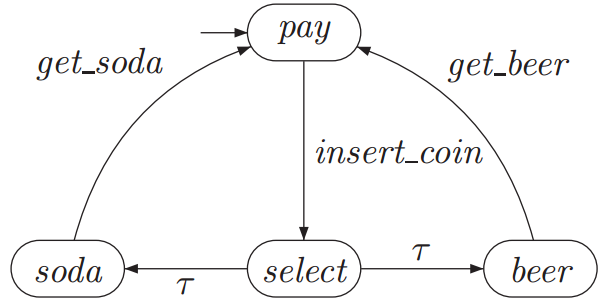
\includegraphics[scale=0.5]{images/exemplts.png}
\caption{Exemple de système à transitions étiquetées \cite{baier2008principles}}
\label{exemplts}
\end{center}
\end{figure}

La figure~\ref{exemplts} représente un système à transitions étiquetées où
\begin{itemize}
\item l'ensemble d'états est $S = (pay, select, beer, soda)$
\item les actions sont $Act = (insert\_coin, \tau, get\_soda, get\_beer)$
\item l'ensemble des transitions est $\rightarrow = (pay\xrightarrow{insert\_coin}{}select, select\xrightarrow{\tau}{}soda, select\xrightarrow{\tau}{}beer, soda\xrightarrow{get\_soda}{}pay, beer\xrightarrow{get\_beer}{}pay)$
\item L'ensemble des états initiaux est $I = (pay)$
\end{itemize}
Cet automate représente donc une machine à vendre des sodas et de la bière. En premier lieu, il faut insérer une pièce, ensuite la machine sélectionne avec une probabilité d’un demi un soda sinon une bière et le donne au client, puis finalement, retourne à l'état initial, l'état d'attente.

%On pourrait déterminer la fonction d'étiquetage comme attribuant à tout état $s$ son nom, $L(s) = \{s\}$. On pourrait aussi vouloir s'assurer que <<La machine libère la boisson seulement si elle a reçu une pièce>>, pour ce faire on définirait la fonction d'étiquetage $L$  comme :
%\begin{center}
%$L(pay) = \emptyset, L(select) = {paid}, L(soda) = L(beer) = {paid, drink}$
%\end{center}

\end{exem}

%Cet exemple montre que la sélection de la fonction d'étiquetage se fait de manière arbitraire. 
Dans l'exemple, l'action $\tau$ représente une action interne à la machine qui n'est pas utile dans sa modélisation, la transition est parfois même dépourvue d'action.\\
%Les propositions atomiques sont choisies en fonction de ce dont on souhaite prouver la propriété. Lors des représentations de ces systèmes, l'ensemble $AP$ est souvent représenté de manière non explicite, et on suppose que $AP \subseteq S$ et donc la fonction d'étiquetage est $L(s) =  \{s\} \cap AP$.\\

Dans la fin de cette sous-section, nous définissons les notions de successeurs et de prédécesseurs itérés qui permettent de représenter tous les états accessibles depuis un élément et tous les états qui ont accès à un élément.


\begin{defin}[Prédécesseur et successeur itéré\cite{baier2008principles}]
On définit $Post^*(s)$ comme étant 
\begin{center}$\underset{i \geq 0}{\cup} Post^i(s)$ avec $Post^0(s) = s$ et $Post^i(s) = Post(Post^{i-1}(s)) \forall i \geq 1$.\\
$Post^+(s)$ est $\underset{i \geq 1}{\cup} Post^i(s)$.
\end{center}
De la même façon, on définit $Pre^*(s)$ comme étant
\begin{center}
$\underset{i \geq 0}{\cup} Pre^i(s)$ avec $Pre^0(s) = s$ et $Pre^i(s) = Pre(Pre^{i-1}(s)) \forall i \geq 1$.\\
$Pre^+(s)$ est $\underset{i \geq 1}{\cup} Pre^i(s)$.
\end{center}

Ces itérations convergent vers un point fixe puisque les opérations impliquées sont monotones et que l'ensemble des états est fini.
\end{defin}

\subsection{Définition du problème}
Pour poser le problème de l'accessibilité correctement il faut encore définir ce qu'est un chemin.

\begin{defin}[Chemin \cite{geeraerts2013multiprocessor}]
Un chemin dans un automate fini $A = (V, E, S_0, F)$ est une séquence finie d'état $v_1, ..., v_t$ telle que, pour tout $1 \leq i \leq t-1 : (v_i, v_{i+1}) \in E$ 
\end{defin}

La fonction $Reach(A)$ découle de cette définition : soit $V' \subseteq V$ un ensemble d'état de $A$, s'il existe un chemin $v_1,...v_t$ dans $A$ tel que $v_t \in V'$, on dit que $v_1$ a accès à $V'$. Pour un automate $A$, on représente l'ensemble des états accessibles depuis un état initial de $A$ par la fonction $Reach(A)$.

\begin{defin}[États accessibles \cite{geeraerts2013multiprocessor}]
L'ensemble des états accessibles d'un automate est défini par 
\begin{center}
$Reach(A) = \{v \in V | \exists\ un\ chemin\ v_1,...,v_t : v_1 \in S_0 \wedge v_t = v\}$
\end{center}
\end{defin}

Dès lors, le problème de l'accessibilité dans un automate pose la question de savoir si, étant donné un automate $A$ et l'ensemble d'états finaux $F$, il est possible d'accéder à un état final dans l'automate $A$, c'est-à-dire, de savoir si $Reach(A) \cap F = \emptyset$ ou non. On peut aussi poser la question par rapport aux prédécesseurs et successeurs itérés :

\begin{theo}[\cite{doyen2010antichain}]
Soit $A = (V,E,S_0,F)$ un automate fini, la réponse au problème de l'accessibilité de $i \in S_0$ à $F$ pour $A$ est Oui si, et seulement si, $Post^*(i) \cap F \neq \emptyset$, si, et seulement si, $\underset{f \in F}{\cup}Pre^*(f) \cap i \neq \emptyset$.
\end{theo}

La complexité en temps, soit la quantité d'opérations nécessaire pour résoudre un problème, de la fonction $Reach$ dépend du modèle utilisé. Dans le cas d'un automate fini, le problème peut se résoudre simplement par une recherche en profondeur ou en largeur, dès lors il est résoluble en temps linéaire par rapport au nombre d'états et de transitions, c'est-à-dire qu'au pire des cas il faudra emprunter toutes les transitions et passer par tous les états. Il en va de même pour les systèmes à transitions étiquetées finis puisqu'il s'agit d'automates finis décorés.\\

Concrètement, on pourrait utiliser le problème de l'accessibilité pour vérifier qu'un programme ne peut jamais atteindre un état erroné. On créerait alors un système à transitions étiquetées $A = (V, E, S_0, F)$ avec $V$ les états du programme, $E$ les transitions du programme, $S_0$ comprenant l'état initial et $F$ l'ensemble des états erronés. On voudrait donc obtenir que $Reach(A) \cap F = \emptyset$, que $\forall i \in S_0 : Post^*(i) \cap F = \emptyset$.

\subsection{Antichaîne}
Soit un automate $A$, la fonction $Reach(A)$ est linéaire en la taille de $A$ mais il est justement possible que celle-ci soit grande. Les automates sont souvent construits pour faire un test exhaustif, comme c'est le cas en model-checking, leurs tailles deviennent alors exponentielles en le nombre de branchements du programme à vérifier, mais, bien souvent, il y a des répétitions dans ces automates fraîchement créés.\\

%\begin{exem}
%Imaginons qu'on cherche à vérifier la bonne exécution d'un programme qui aurait trois instructions indépendances entre elles, les instructions A, B et C ainsi qu'une instruction optionnelle, X. Parmi les différentes exécutions possibles, concentrons-nous sur A;B;C et A;B;C;X.\\

%On commence par vérifier que le scénario A;B;C se passe correctement et ensuite on fait de même pour le second. Lors de ces deux vérifications, la séquence A;B;C a été vérifié deux fois, alors que son comportement sera toujours le même.\\
%On va alors améliorer la performance du test en testant uniquement la séquence A;B;C;X car elle permet de tester l'autre en la simulant directement.
%\end{exem}

%Éviter de parcourir plusieurs fois les mêmes séquences d'états dans un automate généré à partir des instructions d'un logiciel permettrait de mettre en place cette optimisation.\\

Les antichaînes construisent le sous-ensemble des éléments incomparables deux à deux avec une certaine relation d'ordre (autorisant les cycles) d'un ensemble. Nous allons utiliser ces dernières avec une relation d'ordre spécifique pour qu'elles représentent des groupes d'éléments dans l'ensemble de départ. Cette relation d'ordre spécifique est une relation de simulation, cette notion et celle de l'antichaîne sont définies dans cette sous-section, en commençant le plus général, une relation d'ordre spécifique.\\

\begin{defin}[Préordres et leurs propriétés \cite{doyen2010antichain}]
Un préordre sur un ensemble fini $V$ est une relation binaire $\preceq \subseteq V \times V$ (ou $\succeq$) qui est réflexive et transitive. Si $v_1 \preceq v_2$, on dit que $v_1$ est plus petit que $v_2$ (ou que $v_2$ est plus grand que $v_1$).
Un préordre $\preceq'$ est dit plus grossier que $\preceq$ si pour tout $v_1, v_2 \in V$ si $v_1 \preceq v_2$ alors $v_1 \preceq' v_2$.\\
La $\preceq$-fermeture vers le haut d'un ensemble $S \subseteq V$ est l'ensemble $Up(\preceq, S) = \{ v_1 \in V | \exists v_2 \in S : v_2 \preceq v_1 \}$ des éléments qui sont plus grands ou égaux à un élément de $S$.
Un ensemble $S$ est $\preceq$-fermé vers le haut s'il est égal à sa $\preceq$-fermeture vers le haut, $Min(\preceq, S) = \{s_1 \in S | \forall s_2 \in S : v_2 \preceq v_1 \rightarrow v_1 \preceq v_2 \}$ reprend l'ensemble des éléments minimaux de $S$.\\
On remarque que $Min(\preceq, S) \subseteq S \subseteq Up(\preceq, S)$.\\

De la même façon, on définit la $\preceq$-fermeture vers le bas $Down(\preceq, S) = \{ v_1 \in V | \exists v_2 \in S : v_1 \preceq v_2 \}$ d'un ensemble $S$ et on dit que $S$ est $\preceq$-fermé vers le bas si $S = Down(\preceq, S)$ et $Max(\preceq, S) = \{s_1 \in S | \forall s_2 \in S : v_1 \preceq v_2 \rightarrow v_2 \preceq v_1 \}$ est l'ensemble des éléments maximaux de S.

\end{defin}

Maintenant que les préordres sont définis, nous pouvons détailler l'antichaîne se basant dessus.

\begin{defin}[Antichaîne \cite{doyen2010antichain}]
Un ensemble $H \subseteq V$ est une quasi-antichaîne si pour tout $v_1 , v_2 \in S$, soit $v_1$ et $v_2$ sont incomparables, soit $ v_1 \preceq v_2$ et $v_2 \preceq v_1$.\\
Ce même ensemble $H \subseteq V$ est une antichaîne si pour tout $v_1 , v_2 \in S$, $v_1$ et $v_2$ sont incomparables.\\
On obtient alors, une antichaîne avec la relation $\preceq$ est un sous-ensemble $H$ de $V$ tel que :
\begin{center}
$H = \{v_1 \in V|\forall v_2 \in V : v_1 \preceq v_2 \Rightarrow v_1 = v_2\}$
\end{center}

Avec un préordre, les ensembles $Min(\preceq, S)$ et $Max(\preceq, S)$ sont des quasi-antichaînes et avec un ordre partiel, un préordre antisymétrique, ces ensembles sont des antichaînes.\\
Par abus de langage, on appelle antichaîne les ensembles d'éléments minimaux ou maximaux, même s'il ne s'agit pas d'un ordre partiel, mais d'un préordre.

\end{defin}

L'antichaîne nous donne les éléments incomparables d'un ensemble selon un ordre partiel. L'ordre partiel qui nous intéresse est celui de la simulation, c'est celui-là qui nous permettra de représenter plusieurs états d'un automate en un seul.

\begin{defin}[Relation de simulation \cite{doyen2010antichain}]
Soit $A = (V,E,S_0,F)$ un automate fini, on définit deux notions de simulation:
\begin{itemize}
\item un préordre $\preceq_f$ sur $V$ est une simulation vers l'avant pour $A$ si pour tout $v_1, v_2, v_3 \in V$, si $v_2 \preceq_f v_1$ et $(v_1, v_3) \in E$, alors il existe $v_4 \in V$ tel que $v_4 \preceq_f v_3$ et $(v_2, v_4) \in E$.
\item un préordre $\succeq_b$ sur $V$ est une simulation vers l'arrière pour $A$ si pour tout $v_1, v_2, v_3 \in V$, si $v_2 \succeq_b v_1$ et $(v_3, v_1) \in E$, alors il existe $v_4 \in V$ tel que $v_4 \succeq_b v_3$ et $(v_4, v_2) \in E$.
\end{itemize}
\end{defin}

Nous avons maintenant tout ce qu'il nous faut pour résoudre un problème d'accessibilité par antichaîne : l'algorithme par itérations de point fixe, les relations de simulation et les antichaînes.\\
Pour un automate $A = (V,E,S_0,F)$, une fois qu'une relation de simulation $\preceq_f$ est définie, nous sommes en mesure de créer des antichaînes $H \subseteq V$ simulant des états de l'automate $A$. On pourra alors utiliser un algorithme de points fixes qui évitera d'explorer les états représentés par une antichaîne précédemment explorée.\\

En particulier on utilisera une version modifiée de l'algorithme de point fixe $\widehat{P}ost^*(s)$ :

\begin{center}
$\underset{i\geq 0}{\cup} \widehat{P}ost^i(s)$ avec\\
$\widehat{P}ost^0(s) = Min(\preceq_f, s)$\\
$\widehat{P}ost^i(s) = Min(\preceq_f, \widehat{P}ost^{i-1}(s) \cup Post(\widehat{P}ost^{i-1}(s)))\ \forall i \geq 1$\\

\end{center}

Le développement suit la même logique dans le cas d'une simulation vers l'arrière.\\

Cette sous-section se termine en illustrant toutes ces notions avec deux exemples :

\begin{exem}[]
\begin{figure}[!h]
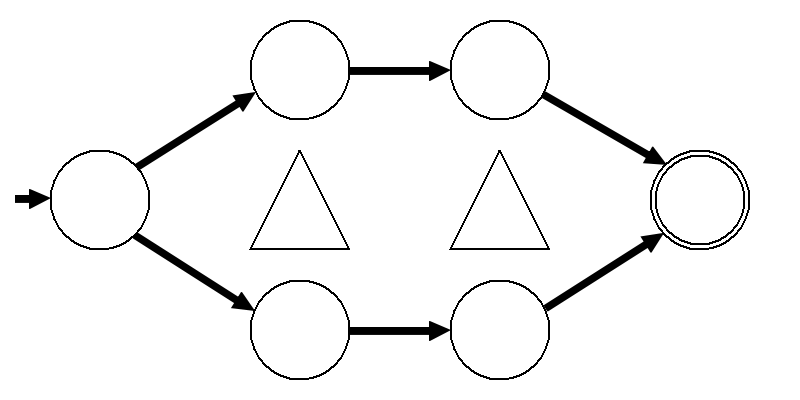
\includegraphics[width=\textwidth]{images/exanti2.png}
\caption{Exemple d'utilisation d'antichaînes}
\label{dfna}
\end{figure}

Cette illustration représente un automate fini, un cercle est un état, une flèche reliant deux cercles est une transition, l'état initial est celui avec la flèche orpheline pointant vers lui et l'état final est le double cercle.\\

Sur l'exemple en figure \ref{dfna}, on souhaite savoir s'il existe un chemin d'un état initial à un état final. Nous avons identifié une relation de simulation vers l'avant $\triangleleft$, sur l'image un état avec la pointe du triangle devant lui simule celui qui a la base devant lui. Nous allons exécuter un algorithme en largeur vers l'avant. A la première itération, on obtiendra alors les deux états succédant l'initial, on utilisera la fonction $Min$ avec la relation de simulation $\triangleleft$ pour garder celui ou ceux qui ne sont simulés par aucun autre et nous continuerons à utiliser les fonctions $Post$ et $Min$ jusqu'à stabilité. Dans l'exemple, nous emprunterons donc le chemin du haut jusqu'à l'état final.

\end{exem}

Un exemple plus concret de l'utilisation de ces antichaînes se retrouve dans le cas du problème de l'universalité :

\begin{exem}[\cite{doyen2010antichain}]
Considérons la construction par sous-ensemble du complément d'un automate non déterministe (NFA) à alphabet fini. Ce complément sera un automate fini déterministe (DFA), ses états seront des groupes d'états du NFA, appelé cellule, noté $s_i$. Dans ce complément, l'inclusion entre les cellules est un ordre partiel et est une relation de simulation vers l'avant\footnote{c'est aussi une simulation vers l'arrière} : si $s_2 \subseteq s_1$ et qu'il y a une transition de $s_1$ vers $s_3$ alors il existe une transition de $s_2$ vers un $s_4 \subseteq s_3$. On retrouve cette propriété dans le problème de l'accessibilité : si $s_2 \subseteq s_1$ et une cellule finale est accessible depuis $s_1$, alors $s_2$ a accès à une cellule finale aussi. Dans ce cas, un algorithme de recherche en largeur vers l'avant pourra se permettre de ne pas explorer $s_1$ s'il explore $s_2$. En effet, $Post^*(s_1) \cap F \neq \emptyset \rightarrow Post^*(s_2) \cap F \neq \emptyset$ ce qui veut dire que si $s_2$ a accès à une cellule finale, c'est soit parce que $s_1$ y a accès, soit par ce que $s_2$ possède un chemin que $s_1$ ne peut emprunter qui mène à une cellule finale. L'algorithme manipule des ensembles $\subseteq$-fermés vers le haut de cellules qui peuvent être représentés par des antichaînes de leurs éléments $\subseteq$-minimaux.\\

C'est par cette méthode que l'article \cite{doyen2010antichain} propose de résoudre le problème de l'universalité pour un NFA, avec lequel la résolution par antichaîne prend tout son sens. On aimerait savoir si un automate non déterministe accepte tous les mots de son alphabet, le but est alors de construire un DFA par sous-ensembles et d'inverser les états finaux. Dès lors, si un état final est accessible par un état initial, cela signifie qu'il existe un mot qui n'est pas accepté par le NFA de base. Dans ce cadre, nous pouvons utiliser la recherche en largeur vers l’avant avec antichaînes basées sur l'inclusion, une relation de simulation vers l'avant.
\end{exem}

\section{Réduction}
Ont été présentés deux problèmes qui semblent différents, de deux domaines différents de l'informatique, pourtant ils peuvent être corrélés. En effet, le but est de résoudre le problème de l'ordonnançabilité à criticité mixte en résolvant celui de l'accessibilité dans un automate. Ces deux problèmes ne sont pas liés tels quels, il va falloir réduire l'un vers l'autre, en l'occurrence, l'ordonnançabilité à criticité mixte vers le l'accessibilité dans un automate.\\

Cette réduction est une passerelle entre deux communautés des sciences informatiques qui n'ont a priori pas à se rencontrer.\\

Il s'agit donc de formaliser l'ordonnancement CM en tant que système à transitions étiquetées. La modélisation se basera sur le travail de Baker et Crinei \cite{bakerbrute}, celle-ci modélise toutes les exécutions possibles d'un système de tâche par les différents chemins possible dans un automate. Cependant, le type d'ordonnancement n'est pas le même. En effet dans le travail de Baker et Crinei, on retrouve un test d'ordonnançabilité pour un système de tâche sporadique en multiprocesseur.\\

Certaines notions restent les mêmes, par exemple on se servira d'état de système, nécessitant de savoir pour chaque travail d'une instance le temps avant leur libération $nat$ et le temps restant de calcul $rct$.

\begin{defin}[État du système \cite{geeraerts2013multiprocessor}]
Étant donné une instance de $n$ travaux $I = (J_1, ..., J_n)$, l'ensemble des états du système est un ensemble de tuples $S = (nat_s, rct_s)$
\begin{itemize}
\item $nat_s$ est une fonction de $I$ vers $\mathbb{N}$ tel que pour tout $J_i : nat_s(J_i) \leq O_{max}$ avec $O_{max} = max_i\ O_i$
\item $rct_s$ est une fonction de $I$ vers $(1,...,C_{max})$ avec $C_{max} = max_i\ C_i$
\end{itemize}

Les états possibles d'une instance $I$ sont représentés par $State(I)$.\\
Ces états semblent infinis, car il n'y a pas de borne inférieure, mais il sera démontré plus tard qu'il y en a bien une.
\end{defin}

Nous remarquons ici que cette définition telle quelle n'est pas adaptée à une instance CM, car elle ne tient pas compte des différents niveaux de criticité, mais elle donne déjà une idée de l'allure qu'elle prendra. Il faudra définir les différents évènements possibles, comme un coup d'horloge ou le passage à une criticité supérieure, tout ceci se retrouvera dans le modèle.







\section{Contribution}

La première étape du mémoire sera de réduire le problème de l'ordonnancement à criticité mixte en problème d'accessibilité dans un automate. Pour ce faire, il faudra créer le modélisme qui permettra de développer tous les différents scénarios d'une instance CM selon un ordonnanceur en tant qu'automate fini.\\

Ensuite, il faudra transformer les états de cet automate en antichaînes dans le but de réduire le temps de parcours du graphe, il faudra donc définir la relation de simulation pour les différents états en tenant compte des contraintes posées par la criticité mixte.\\

Une fois la modélisation terminée, une implémentation logicielle du problème sera mise en place dans le but de tester l'efficacité de la résolution du problème de certification. Ceci sera accompagné de comparatifs entre la méthode de résolution avec et sans antichaînes.



\chapter{Algortihme d'ordonnancement}
\section{Introduction}
Les but de ce chapitre est de présenter différents algorithmes d'ordonnancement d'ensemble de tâche CM sporadique. Cette approche est nécessaire est pour pouvoir les utiliser dans le futur modèle et surtout pour voir s'il est possible de trouver des conditions d'utilisation plus permissive que les présente.

\section{CAPA}

L'algorithme le plus simple est définir la priorité des tâches en fonction de leur criticité, d'où le nom de cette méthode \textit{Criticality As Priority Assignment, CAPA}. L'idée intuitive de l'algorithme est que l'on souhaite éviter de donner du temps d'accès à la ressources à des tâches qui pourrait ne plus être considéré, de criticité inférieure. Cependant cette algorithme peut mener à l'échec d'ordonnancement d'ensemble de tâches même avec une utilisation très faible. Cette faible performance vient de la rigidité de l'assignation des priorité.\cite{de2009scheduling} 

\begin{exem}[\cite{santy2012ordonnancement}]
Considérons l'ensemble de tâches $\tau$ composé de :
\begin{itemize}
\item $\tau_1 = \{0,3,3,1,[1,1]\}$
\item $\tau_2 = \{0,5,5,2,[3,4]\}$
\end{itemize}

L'algorithme \textit{CAPA} assignera statiquement la priorité $\pi(\tau_2) > \pi(\tau_1)$ car $\chi_2 > \chi_1$.

\begin{figure}[h]
\centering
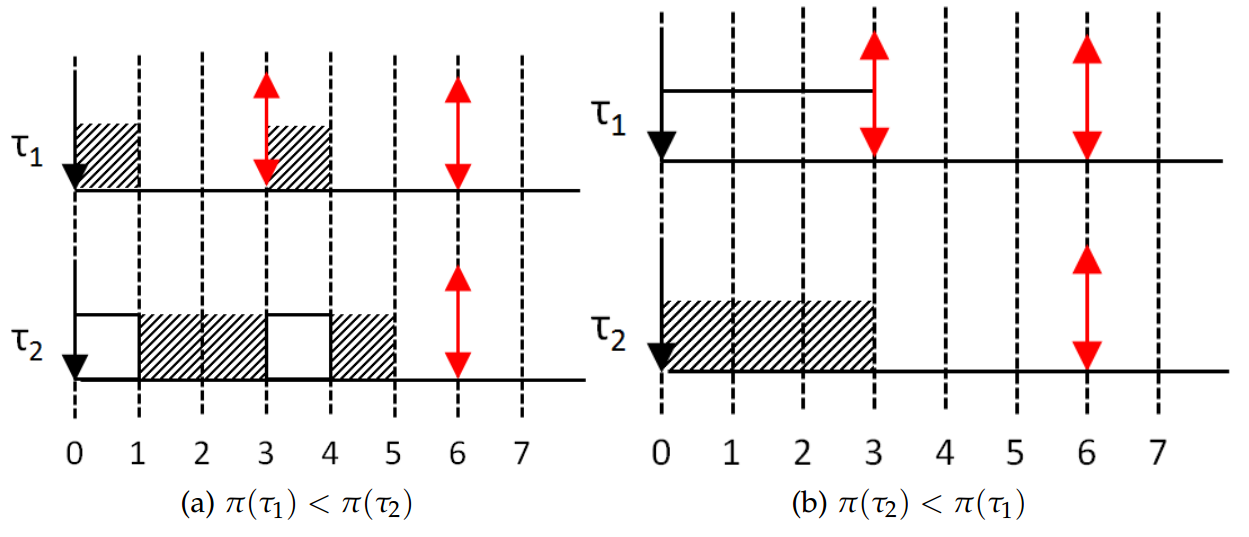
\includegraphics[scale=0.25]{images/capa.png}
\label{ordo:capa}
\caption{Non optimalité de CAPA \cite{santy2012ordonnancement}}
\end{figure}

Dans la \autoref{ordo:capa}, il est apparent que \textit{CAPA} mène à un ordonnancement erroné, alors qu'il est possible d'ordonnancer $\tau$.

\end{exem}

\section{Vestal}
Vestal propose un autre approche\cite{vestal2007preemptive}, basée sur la méthode d'Audsley\cite{audsley1991optimal}. L'algorithme se base sur deux observations, Vestal annonce qu'elles sont maintenue en criticité mixte.

\begin{lem}[\cite{vestal2007preemptive}]
\label{ordo:vestal:low}
Le pire temps de réponse pour un tâche peut être déterminé en sachant quel sous-ensemble de tâche ont une priorité supérieure à elle mais sans avoir besoin de savoir quelle elle l'assignation spécifique de priorité.
\end{lem}

\begin{lem}[\cite{vestal2007preemptive}]
\label{ordo:vestal:higher}
Si un tâche $\tau_i$ est ordonnançable selon une certaine assignation de priorité, elle reste ordonnançable avec une priorité supérieure (les priorités des autres tâches restent identique).
\end{lem}

L'algorithme commence avec l'ensemble de tâche sans priorité. Les priorité sont ensuite assignées de plus faible à la plus forte, de sorte que la première tâche assignée sera le plus fiable prioritaire. À chaque étape, l'algorithme sélectionne une la tâche plus faiblement prioritaire, lui assigne cette priorité et recommence avec l'ensemble des tâches sans cette dernière. Si à un moment aucune tâche n'est éligible à recevoir la priorité la plus faible, alors cette algorithme ne permet d'ordonnancé l'ensemble de tâche.\\

Il est donc nécessaire de déterminer si une tâche peut recevoir la plus faible priorité. Pour ce faire, Vestal propose un test basé sur le temps de réponse qui est faisable par le \autoref{ordo:vestal:low}. 


\begin{defin}[Pire temps de réponse CM \cite{vestal2007preemptive}]
Le pire temps de réponse CM $R_i$ d'une tâche $\tau_i$ est la taille de l'intervalle maximale compris entre la génération d'un de ses travaux et sa complétion. Le temps de réponse ne peut s'obtenir trivialement. Il s'agit de la somme des WCETs des travaux de plus haute priorité de celui de la tâche durant l'intervalle $[t, t+R_i)$ où $t$ est l'instant où le travail est généré :
\begin{equation}
R_i=\underset{\tau_j \in hep(i)}{\sum} \lceil\dfrac{R_i}{T_j}\rceil C_j(\chi_i)
\end{equation}
Où $hep(i)$ est l'ensemble des tâche avec une priorité égale ou  plus élevé que $\tau_i$
\end{defin}

Cette équation récursive peut se résoudre à l'aide d'une itération de point fixe. Il faut comment assigner $R_i := C_i(\chi_i)$ et ensuite, évaluer la partie droite de l'équation jusqu'à stabilisation. A tout instant, si $R_i > D_i$ alors la tâche ne peut avoir la priorité qui lui a été assignée, sous peine d'un ordonnancement défaillant.\\

\subsection{AMC}
Baruah \textit{et al.} ont étendu les travaux de Vestal et ont trouvé un test pour la viabilité d'une tâche à une certaines priorité plus permissif.\cite{baruah2011response}\\

Baruah \textit{et al.} distingue trois l'analyse en trois phase :

\begin{itemize}
\item Vérifier l'ordonnançabilité en criticité $LO$
\item Vérifier l'ordonnançabilité en criticité $HI$
\item Vérifier l'ordonnançabilité du changement de criticité
\end{itemize}

Pour effectuer ces test, une extension du pire temps de réponse CM est fait, prenant en compte la criticité.\\


\begin{defin}[Pire temps de réponse CM en criticité $\ell$ \cite{baruah2011response}]
Le pire temps de réponse CM $R_i$ d'une tâche $\tau_i$ au niveau $\ell$ est la taille de l'intervalle maximale compris entre la génération d'un de ses travaux et sa complétion lors ce que ce travail est généré dans un système de criticité $\ell$. Il s'agit de la somme des WCETs au niveau $\ell$ des tâches toujours présentes de plus haute priorité que celle de la tâche durant l'intervalle $[t, t+R_i)$ où $t$ est l'instant où le travail est généré, et de $C_i(\chi_i)$, le pire temps d'exécution de $\tau_i$ :
\begin{equation}
R_i= C_i(\chi_i) +\underset{\tau_j \in hp(i, \ell)}{\sum} \lceil\dfrac{R_i}{T_j}\rceil C_j(\ell)
\end{equation}
Où $hpH(i, \ell)$ est l'ensemble des tâches de criticité au moins $\ell$, avec une priorité plus élevé que $\tau_i$
\end{defin}

Pour vérifier l'ordonnançabilité en criticté $LO$ et $HI$, on utilise les tests standards : $R_i^{LO} \le D_i \wedge R_i^{HI} \le D_i$.\\


Le temps de réponse CM d'une tâche $\tau_i$ lors d'un changement de criticité est noté $R_i*$. Pour le trouver, on définit l'interférence maximale d'une tâche $HI$-critique si il y a un changement de criticité, généré par une tâche $\tau_s$ à un instant $s$. Le passage au niveau de criticité supérieur est déclenché lors ce qu'un tâche $\tau_s$ s'exécute pour plus longtemps que $C_s(LO)$. Si cette événement impacte $\tau_i$, cela signifie que $s < R^{LO}_i$, et la priorité de $\tau_s$ est supérieure ou égale à celle de $\tau_i$; sinon $\tau_i$ se serait complétée avant le changement de criticité. On crée alors $R^s_i$, le temps de réponse de la tâche $\tau_i$, lors ce qu'un changement de criticité se passe au temps $s$, relativement au temps de génération de $\tau_i$.

\begin{equation}
R_i^s = C_i(HI) + I_L(s) + I_H(s)
\end{equation}

où $I_L(s)$ est l'interférence venant des tâches avec une criticité plus faile que $\tau_i$ et $I_H(s)$ est l'interférence venant des tâches avec une criticité supérieure ou égale à celle de $\tau_i$.\\

Les tâches ce criticité plus faible sont abandonné après $s$ et donc leur interférence est bornée par :
\begin{equation}
I_L(s) = \underset{j \in hp(i, LO)}{\sum} (\left\lfloor \dfrac{s}{T_j} \right\rfloor + 1) C_j(LO)
\end{equation}

La valeur $plancher +1$ est utiliser car dés qu'une tâche est émise, il faut considéré son interférence.\\

Pour l'interférence $I_H(s)$, on supposera que tout les travaux actif au temps $s$, s'exécute pour $C(HI)$ unité de temps. D'où, seule le travaux avec une échéance avant $s$ utilise leur estimation pour la criticité $LO$.\\
Considérons l'interférence d'un tâche $\tau_k$ au temps $t$ avec $t > s$. Le nombre maximum d'émission que la tâche peut faire est $\lceil t / T_k \rceil$. Le nombre maximum d'émission qu'un tâche peut faire durant l'intervale $t$ - $s$ est borné par 
\begin{equation}
\label{amc:nbrel:pess}
\left\lceil \dfrac{t-s-(T_k-D_k)}{T_k} \right\rceil +1
\end{equation}

Cependant, si $s$ et petit et $D_k$ trop proche de $T_k$ alors l'\autoref{amc:nbrel:pess} peut inclure plus de travaux qu'il n'y en a vraiment. On définit donc

\begin{equation}
M(k,s,t) = min \left\lbrace \left\lceil \dfrac{t-s-(T_k-D_k)}{T_k} \right\rceil +1, \left\lceil \dfrac{t}{T_k} \right\rceil \right\rbrace
\end{equation}

L'interférence au temps $t$ est alors

\begin{equation}
I_H(s) = \underset{k \in hp(i, HI)}{\sum} \left( M(k,s,t)C_k(HI) + \left(\left\lfloor \dfrac{t}{T_k} \right\rfloor - M(k,s,t)\right) C_j(LO) \right)
\end{equation}

Et donc 

\begin{equation}
R_i^s = C_i(HI) + \left( \underset{j \in hp(\i, LO)}{\sum} (\left\lfloor \dfrac{s}{T_j} \right\rfloor + 1) C_j(LO) \right) +$$\\$$\underset{k \in hp(i, HI)}{\sum} \left( M(k,s,R_i^s)C_k(HI) + \left(\left\lfloor \dfrac{R_i^s}{T_k} \right\rfloor - M(k,s,R_i^s)\right) C_j(LO) \right)
\end{equation}

Avec

\begin{equation}
R_i* = max(R_i^s) \forall s
\end{equation}

Il reste à trouver quelles sont les $s$ à tester. L'intervalle possible pour $s$ va de $0$ à $R^{LO}_i$. En analysant $R_i^s$, il faut remarque que le terme avec $hp(i, LO)$ augmente avec $s$, alors que le terme avec $hp(i, HI)$ diminue avec $s$. D'où, $R_i^s$ ne peut augmenter que lors ce qu'une tâche $LO$-critique génère un travail, il s'agit donc des points à prendre en compte.


\section{OCBP}

\textit{OCBP} est un algorithme d'ordonnancement basé sur priorités. Cet ordonnanceur fonctionne de manière récursive, en cherchant à assigner une priorité la plus basse à une des tâche et continuer jusqu'à ce que toutes les tâches ait une priorité, dans la même idée que l'algorithme d'Audsley\cite{audsley1991optimal} en ordonnancement temps réel classique. L'algorithme se base uniquement sur le WCET de la criticité d'une tâche, c'est pour ça qu'il s'appel \textit{Own Criticality Based Priority, OCBP}.\\
Une première version de cette algorithme a été imaginée pour un ensemble te travaux, dans cette configuration, l'assignation de priorité se fait hors ligne.\cite{baruah2010towards} Il semble alors évident de simplement appliqué cette version de l'algorithme pour l'instance CM de travaux générée par un ensemble de tâche CM sporadique. Cependant, cette approche n'est pas possible. Premièrement, car la phase hors-ligne d'assignation des priorité peut être infinie car l'instance de travaux généré par l'ensemble de tâches CM sporadique est potentiellement infinie. Ensuite, et surtout, l'algorithme dans sa version sur instance CM requiert d'avoir une spécification précise des travaux, or avec des tâches CM sporadique, il n'est pas possible de savoir exactement quand les travaux seront généré, seul une borne inférieure est disponible.\\
La suite de cette section présente l'algorithme OBCP pour des tâche sporadique présenté en dans le papier \cite{li2010algorithm} mais ne s'attardera pas sur la résolution de des problèmes énoncé, pour les découvrir, consultez ce même papier.\\

\begin{defin}[Instant oisif \cite{goossens1999scheduling}]
$x \in \mathbb{N}$ est un instant oisif de l'ordonnancement d'un système si toutes les requêtes émise strictement avant $x$ ont été complétée, avant ou au temps $x$.
\end{defin}

\begin{defin}[Période occupée \cite{goossens1999scheduling}]
Une période occupée est un intervalle $[a, b)$, tel que $a$ et $b$ sont deux instant oisif, le processeur est occupé dedans et il n'y a pas d'instant oisif intermédiaire. 
\end{defin}

Supposons qu'une période occupée commence à un instant $t_0$, durant l'exécution. A cet instant, il faut assigner une priorité à tout les travaux qui pourrait potentiellement arrivé dans la période occupée commençant à $t_0$, comme si tout les travaux étaient émis au premier instant permis. Pour le bon fonctionnement de l'algorithme \textit{OCBP}, il faut considéré que tout ces travaux sont "généré-tôt". Ce principe est illustré avec un exemple.

\begin{exem}
Supposons q'un tâche $\tau_i$ peut généré trois travaux durant la période occupée commençant à $t_0$. Au plus tôt, cex travaux seront généré au temps $t_0, t_0+T_i, t_0+2*T_i$ respectivement et auront pour échéance $t_0+D_i, t_0+T_i+D_i, t_0+2*T_i+D_i$ respectivement. Considéré ces travaux comme généré-tôt signifie que leur temps d'arrivé sera $t_0$ pour chacun d'entre eux, leurs échéances restent inchangées.\\

${J_i}^n_{i=1}$ dénote tout ces travaux à $t_0$; $J_i = (t_0, d_i, \chi_i, c_i$
\end{exem}


\subsection{Assignation des priorités}

Il faut assigner les priorités aux travaux ${J_i}^n_{i=1}$ conformément à l'assignation de priorité \textit{OCBP}. Cet assignation de priorité est la fonction $\pi : {J_i}^n_{i=1} \rightarrow {1,2,...,n}$.\\

L'assignation \textit{OCBP} fonctionne de la manière suivante :\\
Déterminer au sein d'un instance CM $I$, le travail $J_i$ le plus faiblement prioritaire : un travail $J_i$ peut avoir la priorité la plus faible si
\begin{itemize}
\item c'est un travail $LO-critique$ ($\chi_i = LO$), et il y a au moins $c_i(LO)$ temps entre son émission et son échéance si tout les autres travaux $J_j$ ont une priorité plus élevé et sont exécuté pour $c_j(LO)$ unité de temps; ou
\item c'est un travail $HI-critique$ ($\chi_i = HI$), et il y a au moins $c_i(HI)$ temps entre son émission et son échéance si tout les autres travaux $J_j$ ont une priorité plus élevé et sont exécuté pour $c_j(HI)$ unité de temps.
\end{itemize}
En général, il es possible que plusieurs travaux soit éligible pour être le travail le plus faiblement prioritaire, il faut alors en choisir arbitrairement un. Cet procédure est répétée pour l'ensemble des travaux, sans ce travail avec une priorité fraichement assigné, jusqu'à ce que tout les travaux ait une priorité assignée ou que le travail le plus faiblement prioritaire ne puisse êtres trouvé. Dans ce dernier cas, l'instance $I$ n'est pas \textit{OCBP}-ordonnançable et donc l'ensemble de tâche $\tau$ non plus.

\subsection{Ordonnancement durant l'exécution}

Durant l'exécution, à tout moment, le travail $J_i$ avec la valeur $\pi(J_i)$ la plus faible est qui a été généré mais pas encore signalé comme complété est sélectionné pour exécution. Ce procédé continue jusqu'à l'un des évènement suivant arrive :

\paragraph{E-1}
Un travail $J_i$ s'exécute pour plus que $c_i(LO)$ unité de temps sans signaler sa complétion. Ceci implique que le système est maintenant de criticité $HI$ et que les travaux de criticité $LO$ ne doivent plus être complétés d'ici leurs échéances. Il s'en suit, selon l'exactitude de l'assignation de de priorité \textit{OCBP} à $t_0$, que les travaux de criticité $HI$ qui arriveront durant la période occupée courante sont garantie d'être exécuté jusqu'à leur complétion.

\paragraph{E-2}
Sous not modèle d'ordonnancement basé sur priorité, le processeur est oisif à un certains instant $t$ seulement si tout les travaux qui ont été généré avant $t$ se sont complétés avant ou au temps $t$. Si c'est la cas, la période occupée courant est terminée et les priorité qui ont été au travaux qui n'ont pas été émis sont annulées. Il faut alors attendre la prochaine émission d'un travail, qui va signaler le début d'une nouvelle periode occupée. A ce moment là, il faut recalculer les priorité de tout les travaux qui pourrait arrivé durant cette nouvelle période occupée.

\paragraph{E-3}
L'exécution d'un travail $J_x$ moins prioritaire est préempté à cause de la génération d'un travail de plus haute priorité $J_y$ ($\pi(J_y) < \pi(J_x)$), à l'instant $t_1$. Il faut alors recalculer la fonction de priorité $\pi$ à ce moment précis. Les travaux ayant une priorité plus faible que celle de $J_x$ garderont leur priorité actuelle.\\

Réassignation des priorité : pour tout $i$, soit $\Delta_i$ le nombre de temps d'exécution dont le travail $J_i$ a jouis durant l'intervalle $[t_0, t_1)$. Soit $c_i'(LO) = c_i(LO)-\Delta_i$, $c_i'(HI) = c_i(HI)-\Delta_i$ et $c_i' = [c_i'(LO), c_i'(HI)]$; ceux-ci dénotent le WCET restant pour $J_i$. Il est possible de considéré la charge de travail restant exécutée durant la période occupé comme l'instant 
\begin{equation}
\left\lbrace J_i' = (t_1, d_i, \chi_i, c'_i) \right\rbrace^n_{i=1}
\end{equation}

Supposons que $(n-n')$ travaux ont signalés leurs complétion, durant $[t_0, t_1)$ : ces sont les travaux $J_k$ avec $\pi(J_k) < \pi(J_x)$ car sinon, $J_x$ aurait eu été exécuté avant eux. Soit ${J_i'}^n_{i=1}$ les travaux restant. L'assignation de priorité
\begin{center}
$\pi' : {J_i'}^n_{i=1} \rightarrow {1,2,...n}$
\end{center}
est obtenu depuis $\pi$ comme suit :
\begin{enumerate}
\item Tout les travaux $J_k$ satisfaisant $\pi(J_k) < \pi(J_x)$ qui n'ont pas encore complété leur exécution ont les priorité \textit{OCBP} $\pi'(J_k)$ recalculée sous l'assomption de génération-tôt, qu'ils sont tous généré à l'instant $t_1$
\item Pour tout les travaux $J_k$ satisfaisant $\pi(J_k) \geq \pi(J_x), \pi'(J_k) \leftarrow \pi(J_k) -(n-n')$
\end{enumerate}

L'algorithme est totalement présenté.

\todo{exemple}

\subsection{Test d'ordonnancement}
Il existe une condition suffisante d'ordonnançabilité avec \textit{OCBP} venant de l'article \cite{ekberg2014bounding}, cette sous section la présente.\\

Le test d'ordonnancement se base sur la charge de travaille. Dans les l'ordonnancement temps réel classique, il s'agit du maximum, sur tout les intervalle possible, du temps d'exécution requis cumulé par l'ensemble de tâche, normalisé par l'intervalle \cite{ekberg2014bounding}. Il s'agit donc d'une borne inférieure sur la portion de la capacité d'exécution requise par l'ensemble de tâche pour respecter toutes les échéances.\\
Parallèlement à ce concept, il est possible de définir la charge de travail pour un ensemble de tâche MC à chaque niveau de criticité.

\begin{defin}[Charge $\ell$-critique]
La charge $\ell$-critique d'un ensemble de tâche MC $\tau$ est définie par 
\begin{center}
$Ld_\ell(\tau) = \underset{0\leq t_1 \leq t_2}{max} \left\lbrace \underset{\forall J_i:\chi_i \geq \ell \wedge t_1 \leq a_1\wedge d_1\leq t_2}{\sum} c_i(\ell)/(t_2-t_1) \right\rbrace$
\end{center}
\end{defin}

Pour toute criticité $\ell$, $Ld_\ell(\tau)$ peut-être calculée avec des techniques pour déterminer les charge de travail d'ensemble de tâches traditionnels\cite{Baker05algorithmsfor}. Intuitivement, $Ld_\ell(\tau)$ représente une borne inférieure sur la portion de capacité d'exécution requise par cet ensemble de tâche CM avec lequel il peut respecter ses toutes échéances sujet seulement à la certification au niveau de criticité $\ell$. Pour exécuter correctement un ensemble de tâche CM sporadique, une condition nécéssaire es que cette portion de capacité d'exéctuion requise ne dépasse pas 1.\\

Dans, cette section, \textit{OCBP} est présenté dans le contexte d'un système à criticité double uniquement. Cependant, cet algorithme peut être facilement étendu pour gérer un ensemble de tâche CM sporadique avec plus de deux niveau de criticité. Il est alors possible d'utiliser les connaissances veant de \cite{baruah2010mixed} pour obtenir le test d'ordonnancement CM suivant :

\begin{equation}
\label{test:ocbp}
\forall \ell \in [1,K] : Ld_\ell \le LoadBound(K)
\end{equation}

Où $Ld_\ell$ est la charge au niveau de criticité $\ell$, et $LoadBound(K)$ est une fonction avec respect du nombre total de niveau criticité $K$ du système, qui est calculée récursivement :
\begin{center}
$LoadBound(1) = 1$\\
$LoadBound(K) = \dfrac{2}{1+\sqrt{4\dfrac{1}{Loadbound(K-1)^2}+1}}$

\end{center}

Pour le cas spécial où $K = 2$, une condition sur la charge plus précise est disponible \cite{li2010load}
\begin{equation}
(Ld_2(\tau))^2+Ld_1(\tau) \le 1
\end{equation}

Voilà qui offre un test d'ordonnançabilité pour \textit{OCBP}.

\subsection{Taille de la période occupée}

Lors de l'ordonnancement, il est nécéssaire de connaître la taille de la période occupée pour assigner les priorité aux travaux qui y figure. \cite{li2010algorithm} propose une borne supérieure.\\

La taille de période occupé est divisé en deux. Premièrement, $x_1$ est l'intervalle commençant au début le période occupée jusqu'au moment où un travail dépasse son WCET de criticité $LO$, s'il y en a un. Ensuite, $x_2$ est l'intervalle qui commence à la fin de $x_1$ et se termine à la fin de période occupée.\\

Soit $D_{max} = max_i D_i$. Tout les travaux exécuté pendant $[0, x_1)$ ont leur temps de génération et leur échéance durant l'intervalle $[0, x_1+D_max]$, d'où
\begin{equation}
x_1 \le Ld_{LO}(\tau)(D_{max}+x_1)$$
$$x_1(1-Ld_{LO}(\tau))\le LD_{LO} \times D_{max}$$
$$x_1 <_le \dfrac{Ld_{LO}(\tau)}{1-Ld_{LO}(\tau)} \times D_{max}
\end{equation}

Vu que tout les travaux exécuté durant $[x_1, x_1+x_2)$ ont leurs temps de génération et leur échéance durant l'intervalle $[x_1, x_1+x_2+D_max]$, on en déduit que

\begin{equation}
x_2 \le Ld_{HI}(\tau)(D_{max} + x_1+x_2) $$
$$x_2(1-Ld_{HI}(\tau)) \le Ld_{HI}(\tau)\times(D_{max}+x_1)$$\
$$x_2 \le \dfrac{Ld_{HI}(\tau)}{1-Ld_{HI}(\tau)} \times (D_{max} +x_1)$$\
$$x_2 \le \dfrac{Ld_{HI}(\tau)}{1-Ld_{HI}(\tau)} \times (D_{max} + \dfrac{Ld_{LO}(\tau)}{1-Ld_{LO}(\tau)} \times D_{max})$$
$$x_2 \le \dfrac{Ld_{HI}(\tau)}{(1-Ld_{HI}(\tau))(1-Ld_{LO}(\tau))} \times D_{max}
\end{equation}

La taille de la plus grande période occupé est donc bornée par $x_1+x_2$. Une fois la que période occupé est bornée, il facile d'obtenir les travaux qui peuvent s'y générer.

\section{PLRS et LPA}
\textit{PLRS} est une extension d'\textit{OCBP}, mais considère les instants critique de manière plus abstraite pour alléger le temps calcul. \textit{LPA} est une extension de \textit{PLRS}, qui utilise notamment une taille maximale de période occupée plus restreinte. Ces deux algorithme étant fort proche de l'initial, cette sous-section ne fera que présenter leurs conditions suffisante d'ordonnancement.

\paragraph{PLRS} commence par faire une assignation de priorité intial et la modifiera en ligne. S'il est possible d'assigner à un ensemble de tâche cette assignation initial, il est ordonnançable CM avec \textit{PLRS}\cite{guan2011effective}. Cette assignation est en fait la même que celle pour \textit{OCBP}. Guan \textit{et al.} propose d'utiliser la formulation : chaque tâche $\tau_k$ a un nombre $\delta_k$ représentant le nombre de ses travaux, qu'elle générera durant la période occupée au maximum, qui n'ont pas encore de priorité assigné. Initialement, $\delta_k$ vaut donc le nombre de travaux que la tâche $\tau_k$ générera durant la période occupée au maximum L'algorithme commence par décider quelle travail ayant l'index le plus élevé peux recevoir la priorité la plus faible. Le travail $J^{\delta_k}_k$ est éligible à recevoir la priorité la plus faible si

\begin{equation}
\underset{\tau_j \in \tau}{\sum} (\delta_j \times C_j(\chi_k)) \le (\delta_k-1) \times T_k + D_k
\end{equation}

La partie gauche de l'inéquation représente la charge de travail restante des travaux présent dans l'instance CM composé des travaux généré par les tache présente dans $\tau$ durant la période occupée maximale, si le système est de criticité $\chi_k$. La partie de droite de l'inéquation est la distance minimale entre l'échéance absolue de $J^{\delta_k}_k$ et le début la période occupée considérée. Si plusieurs travaux peuvent recevoir la priorité la plus faible, il faut en choisir un arbitrairement. Une fois ce travail le plus faiblement prioritaire désigné, il faut décrément $\delta_k$ d'une unité pour exclure ce travail lors des prochaines étape. La période occupée maximale est la même que celle dans \textit{OCBP}.\\
Par la suite, l'algorithme itère jusqu'à ce que tout les travaux aient un priorité. Si ce n'est pas possible, alors l'ensemble de tâche n'est pas ordonnançable avec \textit{PLRS}. Attention, bien que si un ensemble de tâche passe cette assignation signifie qu'il est ordonnançable avec \textit{PLRS}, cette assignation en tant que tel ne fonctionnera pas forcément. En effet, l'algorithme modifiera les priorité en ligne, cette partie est consultable en \cite{guan2011effective}.


\paragraph{LPA} , en fidèle succèsseur d'\textit{OCBP}, commence par faire une assignation de priorité hors ligne. Il s'agit de la même que \textit{PLRS}. A nouveau, si une ensemble de tâche passe cette assignation, alors il est ordonnançable avec \textit{LPA} \cite{gu2013improving}. Ici, Gu \textit{et al.} propose une nouvelle façons de calculer la taille de la période maximale.\\

Gu \textit{et al.} définissent la charge $\ell$-critique comme la borne supérieure de la charge total des tâches dont la criticité n'est pas supérieure à $\ell$, dans toute les période occupée, où la criticité ne dépasse pas $\ell$. D'où $Ld_K$ est la borne supérieure pour la tailles des périodes occupés pour l'ensemble de tâche $\tau$. Et ils posent $Ld_0 = 0$.\\

Ensuites, ils prouvent le théorème suivant.

\begin{theo}[\cite{gu2013improving}]
Etant donnée un ensemble de tâches CM sporadiques $\tau$ et la charge $\ell-1$-critique $Ld_{\ell-1}$, on a:
\begin{equation}
\phi_\ell = \dfrac{Ld_{\ell-1} + \sum_{\chi_i \ge \ell} C_i(\ell)}{1 - \sum_{\chi_i \ge \ell} \dfrac{C_i(\ell)}{T_i}}
\end{equation}
\begin{equation}
Ld_\ell = Ld_{\ell-1} + \underset{\chi_i \ell}{\sum}C_i(\ell) \times \left( 1 + \left\lfloor \dfrac{\phi_\ell}{T_i} \right\rfloor \right)
\end{equation}
\end{theo}

Depuis ce théoreme, Gu \textit{et al.} propose l'agorithme suivant pour calculer la charge et ensuite réutilise la manière de créer la période occupé d'\textit{OCBP}, en utilisant leur nouvelle façons de calculer la charge.


\begin{algorithm}[caption={Calcul la charge $\ell$-critique}, label={alg1},mathescape=true]
ComputeGamma($\ell$)
 if $\ell = 0$ then
  return 0
 endif
 $\displaystyle Ld_\ell \gets $ComputeGamma($\ell-1$)
 $\displaystyle \gamma \gets \dfrac{Ld_\ell + \sum_{\chi_i \geq \ell} C_i(\ell)}{1-\sum_{\chi_i \geq \ell} \dfrac{C_i(\ell)}{T_i}}$
 
 return $\displaystyle Ld_{\ell-1} + \sum_{\chi_i = \ell}C_i(\ell) \times \left( 1 + \left\lfloor \dfrac{\gamma_\ell}{T_i} \right\rfloor \right)$
       
\end{algorithm}

\section{EDF-VD}
babruah \textit{et al.} propose un algorithme\cite{BaruahBDMSS11} qui est une variant de \textit{EDF}, appelé \textit{EDF} à échéance virtuel, \textit{EDF-VD}, pour \textit{Virtual Deadlines}.

Pour la compréhension de l'algorithme, l'explication qui suit considère un ensemble de tâche avec une criticité double. Il faut distinguer deux cas.

\begin{itemize}
\item Cas 1. $U_1(1) + U_2(2) \le 1$ : appliquer \textit{EDF} avec les échéances des tâches non modifiée. Dès que le système passe au niveau 2, abandonné les tâches de niveau 1.

\item Cas 2. $U_1(1) + \dfrac{U_2(1)}{1-U_2(2)} \le 1$ et le cas 1 n'est pas satisfait : $\lambda = \dfrac{U_2(1)}{1-U_1(1)}$. Lors ce que le système est en criticité 1 : pour tout tâches $\tau_i$ avec $\chi_i = 2, \widehat{p}_i = \lambda p_i$. Redéfinir les les échéances des tâche tel que $\chi_i = 2$ en y ajoutant $\widehat{p}_i$ au temps des génération de chacun de leurs travails. Ne pas modifier les échéance de tâche avec $\chi _i =1$ et appliquer \textit{EDF}. Lors ce que le système atteint la criticité de niveau 2, abandonner les tâche de criticité de niveau 1 et réinitialiser les échéances des tâches encore considérés et appliquer \textit{EDF} sur ces échéances initiales.
\end{itemize}

Baruah \textit{et al.} donne ensuite un condition suffisante d'ordonnançabilité :

\begin{theo}[\cite{BaruahBDMSS11}]
Si $\tau$ satisfait
\begin{center}
$U_1(1) + min \left( U_2(2), \dfrac{U_2(1)}{1-U_2(2)} \right) \le 1$
\end{center}
Alors $\tau$ est ordonnançable avec \textit{EDF-VD}.
\end{theo}

\section{Greedy}
Ekberg \textit{et al.} ont proposé un algorithme sur l'analyse de la demande des tâches CM\cite{ekberg2014bounding}, cette le section présente.\\

Une approche connue pour être dans l'analyse de l'ordonnancement de charge temps réel est d'utiliser une fonction de borne de demande \cite{baruah1990preemptively}. Une fonction de borne de demande capture la demande d'exécution maximale  d'une tâche durant un intervalle d'un taille donnée.

\begin{defin}[Fonction de borne de demande \cite{ekberg2014bounding}]
Une fonction de borne de demande $dbf(\tau_i, \Delta)$ donne une borne supérieure pour la demande d'exécution maximale possible d'un tâche $\tau_i$ dans tout les intervalle de temps d'une taille $\Delta$, où la demande est calculée comme le temps d'exécution requis total des travaux avec leur fenêtre d'ordonnancement complètement dans l'intervalle.
\end{defin}

Un concept similaire est la fonction de borne d'approvisionnement $sbf(\Delta)$ qui borne inférieurement la quantité de temps d'exécution fournie par le processeur dans tous intervalles de taille $\Delta$. Par exemple, sur un processeur à vitesse unitaire, $sbf(\Delta) = \Delta$.\\

Ce qui rend les fonction de borne de demande et d'approvisionnement intéressante est la proposition suivante :

\begin{prop}
\label{greedy:class:dbfsbf}
Un ensemble de tâche $\tau$ (sans criticité mixte) est ordonnançable par \textit{EDF} sur monoprocesseur avec la fonction de borne inférieure $sbf$ si :
\begin{center}
$ \forall \Delta \ge 0 : \underset{\tau_i \in \tau}{\sum}dbf(\tau_i, \Delta) \le sbf(\Delta)$
\end{center}
\end{prop}

Ekbeg \textit{et al.} étendent l'idée de la fonction de borne de demande à la criticité mixte, avec double criticité. Pour toutes tâche, ils construisent deux fonctions de borne de demande, $dbf_{LO}$ et $dbf_{HI}$, pour les mode de critcité bas et haut respectivement. La \autoref{greedy:class:dbfsbf} est étendue :

\begin{prop}
\label{greedy:mc:dbfsbf}
Un ensemble de tâche $\tau$ (sans criticité mixte) est ordonnançable par \textit{EDF} sur un processeur avec la fonction de borne inférieure $sbf_{LO}$ dans le mode à criticité basse et $sbf_{HI}$ dans le mode à criticité haute si les deux conditions suivante son satisfaite :
\begin{center}
\textbf{\textit{Condition A:}}$\quad \forall \Delta \ge 0 : \underset{\tau_i \in \tau}{\sum}dbf_{LO}(\tau_i, \Delta) \le sbf_{LO}(\Delta)$\\
\textbf{\textit{Condition B:}}$\quad \forall \Delta \ge 0 : \underset{\tau_i \in \tau}{\sum}dbf_{HI}(\tau_i, \Delta) \le sbf_{HI}(\Delta)$
\end{center}
\end{prop}

Les conditions A et B s'assure de l'ordonnançabilité de l'ensemble de tâche en basse et haute criticité. Bien que ces deux modes puissent être analysé séparément avec les conditions ci-dessus, la demande en haute criticité dépend de ce qui se passe en basse criticité.\\

Pour trouver ces fonctions de borne de demande, on suppose, sans perte de généralité, que $sbf_{LO}$ est de vitesse unitaire au maximum.\\
Dans le cas de la criticité basse, l'exercice est simple. Dans ce mode, les tâche $\tau_i$ se comporte comme des tâche sporadique normale, et tout leurs travaux finissent, au pire, après $C_i(LO)$ unités de temps. Il est donc possible d'utiliser des méthodes standard pour calculer les fonctions de borne de demande pour tâche sporadique \cite{baruah1990preemptively}.\\

Avec $dbf_{HI}$, c'est plus compliqué  car il faut considérer les travaux de criticité haute qui ont été actif durant le changement de criticité.

\begin{defin}[Travaux transféré \cite{ekberg2014bounding}]
Un travail émis par une tâche à haute criticité  qui est actif (généré mais non terminé) au moment du changement de criticité est appelé un travail transféré.
\end{defin}

\subsection{Analyser la demande des travaux transférés}
En haute criticité, il faut finir l'exécution restante des travaux transférés avant leur échéance. La demande de ces travaux transféré doit donc être prise en considération dans chaque $dbf_{HI}$ des tâches de haute criticité. Conceptuellement, lors de l'analyse de l'ordonnançabilité en haute criticité, on peut considérer les travaux transféré comme des travaux ayant été généré lors du changement de criticité. Cependant, la fenêtre d'ordonnancement devient l'intervalle entre le changement de criticité et l'échéance du travail, et peut donc être plus courte que d'autres travaux généré par la même tâche. Parceque ces travaux ont pu déjà être pour quelques unités de temps, le temps restant de calcul peut être inférieure à ceux des autres travaux.\\

%fig 1

Pour borner la demande en haute criticité (condition B), on suppose que la demande en basse criticité est approvisionné, sinon l'ensemble de tâche ne peut être ordonnançable. Il s'agit donc de prouver $A \wedge (A \rightarrow B)$, ce qui permettra d'affirmer $A\wedge B$.\\

Analysons les informations disponible sur les travaux transférés. Au moment du passage vers la criticité supérieure, un travail transféré d'un tâche à haute criticité $\tau_i$ a $n\ge 0$ unité de temps restantes avant son échéance. La fenêtre d'ordonnancement restante du travail est de taille $n$. Puisque le travail aurait respecté son échéance en basse criticité, si le changement n'avait pas eu lieu, il peut y avoir au maximum $n$ unité de temps restante de son WCET de bas niveau $C_i(LO)$ au moment du changement. Le travail aura donc été exécuté duran au moins $C_i(LO) -n$ unités de temps avant le changement de criticité. Comme le système est maintenant en haute criticité, le travail doit accomplir jusqu'à $C_i(HI)$ unité de temps au total. Après le changement de criticité, le temps restant d'exécution total pour un travail transféré, après le changement est au plus $C_i(HI) - (C_I(LO)-n)$. Malheureusement, quand $n$ devient petit, la demande est de plus en plus difficile à respecter et mène à $dbf_{HI}(\tau_i,0) = C_i(HI) - C_I(LO)$ dans le cas extrême. Clairement, un tel fonction de borne de demande ne peut satisfaire la condition B.

\subsection{Ajuster la demande des travaux transférés}

Le problème ci-dessus vient du fait que \textit{EDF} peut exécuter des travaux de haute criticité tard lors ce que le système est en basse criticité. Quand le passage à la haute criticité est déclenché, un travail transféré peut avoir un petite fenêtre d'ordonnancement dans laquelle il doit terminer sa demande de haute criticité. Pour augmenter la taille de sa fenêtre d'ordonnancement restante, Ekberg \textit{et al.} propose de séparer les échéances relatives en basse et haute criticité. Pour un tâche $\tau_i$, \textit{EDF} utilisera alors l'échéance relative $D_i(LO)$ et $D_i(HI)$, tel que si un travail est émis au temps $t$, la priorité assigné par \textit{EDF} est basé sur la valeur de $t+D_i(LO)$ pendant la basse criticité et $t+D_i(HI)$ durant la haute criticité.\\

Diminuer l'échéance d'une tâche ne pose pas de problème car respecté une échéance plus strict que l'initial garantie que cette dernière est respectée aussi. En diminuant $D_i(LO)$, il est possible de gagner du temps supplémentaire dans la fenêtre d'ordonnancement des travaux transférés au pris d'empirer la demande en basse criticité. Il faut donc $D_i(LO) = D_i$ si $\chi_i = LO$ et $D_i(LO) \le D_i(HI) = D_i$ si $\chi_i = HI$. Aussi, il est nécessaire que $C_i(LO) \le D_i(LO)$, comme pour l'échéance initial. $D_i(LO)$ n'est pas une vrais échéance dans le sens où son non respect n'entraîne pas un échec d'ordonnancement. Cependant elle est appelé échéance car elle permet de construire $dbf_{LO}$ et elle est utilisé par \textit{EDF} en basse criticité comme s'il s'agissait de l'échéance relative.

\begin{lem}[La demande des travaux transférés \cite{ekberg2014bounding}]
\label{greedy:dtt}
En supposant qu'\textit{EDF} utilise les échéance $D_i(LO)$ et $D_i(HI)$ avec $D_i(LO) \le D_i(HI) = D_i$ pour une tâche $\tau_i$ à haute criticité, et qu'il est garantie que la demande en basse criticité est fournie (en utilisant $D_i(LO)$). Si le changement de criticité se passe lors ce qu'un travail de $\tau_i$ a $n$ unités de temps avant son échéance réelle, alors on sait que :

\begin{enumerate}
\item  Si $n < D_i(HI) - D_i(LO)$, le travail a été terminé avant le passage à la haute criticité.
\item Si $n \ge D_i(HI)-D_i(LO)$, le travail peut être un travail transféré, et a au moins $max \left(0, C_i(LO) - n + D_i(HI) - D_i(LO)\right)$ unités de temps de son exécution ont été finie avant le passage à haute criticité.
\end{enumerate}
\end{lem}

La preuve du lemme est disponible dans l'article dont il vient. Pour la suite il faut maintenant monter comment définir $dbf_{LO}(\tau_i, \Delta)$ et $dbf_{HI}(\tau_i, \Delta)$ avec un $D_i(LO)$ donné.

\subsection{Formulation des fonction de borne de demande}

Il est déjà établi que lors ce que le système est en basse criticité se toute taches $\tau_i$ comporte comme une tâche sporadique classique, avec les paramètres $C_i(LO), D_i(LO), T_i$. La fonction de borne de demande serrée est 
\begin{equation}
dbf_{LO}(\tau_i, \Delta) \overset{def}{=} max \left( 0, \left( \left\lfloor \dfrac{\Delta-D_i(LO)}{T_i} \right\rfloor +1 \right) \times C_i(LO) \right)
\end{equation}

La fonction de borne de demande pour les tâches en haute criticité, $dbf_{HI}(\tau_i, \Delta)$, doit borner supérieurement la demande d'exécution maximale des travaux de $\tau_i$ avec une fenêtre d'ordonnancement dans un des intervalle de taille $\Delta$. Il peut donc y avoir un travail transféré. Par le \autoref{greedy:dtt}, on sait que la fenêtre restante d'ordonnancement d'un travail transféré de $\tau_i$ est au moins de taille $D_i(HI) - D_i(LO)$ unités de temps. L'intervalle de temps $D_i(HI) - D_i(LO)$ est donc l'intervalle minimal dans lequel un fenêtre d'ordonnancement d'un travail de $\tau_i$ peut rentrer. Plus généralement, la taille du plus petit intervalle dans lequel peuvent rentrer $k$ travaux de $\tau_i$ est $(D_i(JI)-D_i(LO))+(k-1)*T_i$. La demande d'exécution de $\tau_i$ durant un intervalle de taille $\Delta$ est donc bornée par :
\begin{center}
$full(\tau_i, \Delta) \overset{def}{=} max \left(0,  \left( \left\lfloor \dfrac{\Delta - (D_i(HI) - D_i(LO))}{T_i}\right\rfloor +1 \right) \times C_i(Hi) \right)$
\end{center}

La fonction $full(\tau_i, \Delta)$ ne tient pas compte qu'un travail transféré ait pu être exécuté pour quelque unités de temps durant la basse criticité. Il est possible de vérifier si tout les travaux qui contribuent à la demande d'exécution $full(\tau_i, \Delta)$ peuvent inséré leur fenêtre d'ordonnancement dans un intervalle de taille $\Delta$ sans considéré un éventuel travail transféré. Pour ce faire, il faut soustraire le temps d'exécution effectué en basse criticité à $full(\tau_i, \Delta)$.\\

Pour un temps d'intervalle $\Delta$, il peut y avoir au plus $n = \Delta mod T_i$ unités de temps restante pour le premier travail, potentiellement un travail transféré. Si $n \ge D_i(HI)$, il y a assez de place pour la fenêtre d'ordonnancement d'un travail complet et rien ne peut être soustrait de $full(\tau_i, \Delta)$. Si $n < D_i(HI) - D_i(LO)$, alors les travaux contribuant à $full(\tau_i, \Delta)$ peuvent placer leur période entière dan l'intervalle, donc rien n'est à soustraire. Sinon, on utilise le \autoref{greedy:dtt} pour quantifier le temps de calcul a soustraire :
\begin{center}
$$
done(\tau_i, \Delta) = \left\{
    \begin{array}{ll}
        max(0, C_i(LO)-n+D_i(HI) - D_i(LO) & si\ D_i(HI) > n \ge D_i(HI) - D_i(LO) \\
        0 & \mbox{sinon.}
    \end{array}
\right.
$$
\end{center}
avec $n = \Delta\ mod\ T_i$.\\
Les deux termes peuvent maintenant être combiné pour obtenir $dbf(\tau_i, \Delta)$ :
\begin{equation}
dbf(\tau_i, \Delta) = full(\tau_i, \Delta) - done(\tau_i, \Delta)
\end{equation}

\subsection{Réglage efficient des échéance relative}

A présent, il faut définir $D_i(LO)$ pou les tâches. Il n'est pas envisageable de tester tout les combinaisons de leur valeurs, car, bien que borné, cet ensemble est exponentiel. Ekberg \textit{et al.} propose une heuristique pour régler ces échéance relative.\\

Leur algorithme se base sur le lemme qui suit :

\begin{lem}[\cite{ekberg2012outstanding}]
Si deux tâches $\tau_i$ et $\tau_j$ de haute criticité sont identique sauf que $D_i(LO) = D_j(LO) - \delta$ pour $\delta \in \mathbb{Z}$ alors :
\begin{center}

$dbf_{LO}(\tau_i, \Delta) = dbf_{LO}(\tau_j, \Delta + \delta) $\\
$dbf_{HI}(\tau_i, \Delta) = dbf_{HI}(\tau_j, \Delta - \delta)$

\end{center} 
\end{lem}

Ce lemme signifie qu'en diminuant $D_i(LO)$ de $\delta$, il est permis de bouger $dbf_{HI}(\tau_i, \Delta)$ par $\delta$ pas vers la gauche au prix de bouger $dbf_{LO}(\tau_i, \Delta)$ par $\delta$ pas vers la droite. En d'autre terme, il s'agit de déplacer $dbf_{LO}$ et $dbf_{HI}$ en espérant trouver une configuration où la demande totale de l'ensemble de tâche est fournie en basse et haute criticité.\\

L'algorithme complet est disponible dans \cite{ekberg2012outstanding}.

\section{LWLF}
Dans la littérature, en ordonnancement temps réel, il existe encore un type d'algorithme qui n'a pas encore utilisé pour l'ordonnancement en criticité mixte. Il s'agit de \textit{LLF, Least Laxity First}.\\

\textit{LLF} est un algorithme d'ordonnancement DP. Il assigne aux travaux une priorité proportionnelle à leur laxité.

\begin{defin}[Laxité\cite{goossens1999scheduling}]
La laxité d'un travail est le temps maximale durant lequel il peut se permettre d'être oisif sans dépasser son échéance.
\end{defin}

Pour la criticité mixte, il faut définir la notion de pire laxité.

\begin{defin}[Pire laxité]
La pire laxité d'un travail est le temps maximale durant lequel il peut se permettre d'être oisif sans dépasser son échéance, pour son pire WCET.
\end{defin}

\textit{LWLF, Least Worst Laxity First}, ordonnance donc les travaux en leur attribuant un une priorité inversement proportionnelle à leur pire laxité.


\chapter{Sémantique sous forme d'automate}

Dans cette section...

\section{Tache Périodique}

Le but de cette section est de modéliser les différentes exécutions d'un ensemble de tâches périodique en criticité mixte, ordonnancé par un algorithme donné, sous la forme d'un automate fini.\\
Il s'agit, dans premier temps, de définir les états qui composent l'automate et puis, de déterminer les transitions entre ceux-ci.\\

Pour représenter un ensemble de tâche durant, il faut qu'il soit possible d'y retrouver les caractéristiques des tâches et le scénario. Pour ce faire, on établi l'état du système comme reprenant ces caractéristique. Pour le scénario dans lequel on se trouve, il suffit d'y inclure le niveau de criticité lors de l'exécution. Il faut ensuite pouvoir définir où les tâches sont dans leur exécution et quand elles doivent être terminée au plus tard.

\begin{defin}[État du système]
Soit $\tau = \tau_1, \tau_2, \tau_3 ...$ un ensemble de tâches périodiques en criticité mixte, l'état du système de $\tau$ est le tuple $S = (at_S, rct_S, crit_S)$ avec

\begin{itemize}
\item $at_S$, une fonction représentant le temps d'arrivée du travail courant d'une tâche : $\tau \rightarrow \mathbb{N},\ at_S(\tau_i) \leq R_{max}$ avec $R_{max} = max(max_i\ (T_i),\ max_i\ (O_i))$
\item $rct_S$, le temps de calcul restant du travail généré par une tâche : $ \tau \rightarrow \mathbb{N},\ 0 \leq rct_S(\tau_i) \leq C_{max}$ avec $C_{max} = max_{i,j}\ C_i(j)$
\item $crit_S$, le niveau de criticité actuel du scénario, $ \in \mathbb{N},\ 1 \leq crit_S \leq K$

\end{itemize}


Cette définition reprend correctement les caractéristiques dont l'état du système à besoin. Le temps d'arrivé des tâche permet de savoir quand la tâche à émise un travail et donc d'en déduire son échéance. Le temps de restant de calcul permet de savoir où la tâche en est dans son exécution. Enfin, le niveau de criticité du scénario est représenté tel quel.\\

L'automate sera composé ces états du système comme états. On remarque que $at_S$ n'est pas borné inférieurement dans la définition, l'automate semble alors infini. Il est possible de finir l'ensemble des états du système et ce sera démontré par la suite.\\
En regardant la définition, il est possible d'avoir des état du système qui ne sont pas cohérent avec un l'ordonnancement d'un ensemble de tâche. Par exemple, il est possible que le temps restant de calcul d'un tâche de criticité inférieure à celle du scénario soit positive. Il s'agirait d'un contradiction avec la définition de l'ordonnancement en criticité mixte. Les transitions de l'automate seront tel que ce genre d'état ne sera jamais atteint.

\end{defin}

Avant de pouvoir définir les transitions de l'automate, il faut établir des notions auxiliaires sur lesquelles elles se baseront.\\
La première de celles-ci est l'ensemble des tâche active, il s'agit des tâches qui souhaitent prendre possession de processeur. De plus, l'ensemble des tâches abandonné dans le scénario. 

\begin{defin}[Tâches actives et abandonnés]
\label{per:actdisc}
Une tâche est dite abandonné lors ce que sa criticité est inférieure à celle de l'état du système. De par la définition de l'ordonnancement en criticité mixte, ces tâches ne font plus partie de celles à ordonnancer. Les tâches abandonnées sont représentées dans le système comme venant de soumettre un travail ne nécessitant aucune ressource..

$Discarded(S) = \{\tau_i | at_S(\tau_i) == 0 \wedge rct_S(\tau_i) == 0\}$\\

Une tâche est active dans l'état $S$ si a émise un travail dans celui-ci et n'est pas été abandonné.

$Active(S) = \{\tau_i | at_S(\tau_i) < 0\vee (at_S(\tau_i) == 0 \wedge rct_S(\tau_i) > 0)\}$\\

Si une tâche génère un travail et que celui si est complété, la définition tel quel qualifierait toujours ces tâches d'active. Cependant, le système de transition sera construit de sort que lors ce qu'une tâche à terminer un travail, son temps d'arrivé deviendra celui du prochain travail.\\
Deux cas seront possible, soit le temps d'arrivé est dans le futur et donc la tâche ne sera plus active. Soit le temps d'arrivé est immédiat, c'est à dire que le travail s'est terminé juste avant la soumission d'un nouveau travail et donc la tâche restera active.
\end{defin}

En ordonnancement en criticité mixte, les tâches signalent leur complétion. Ce type d'ordonnancement fait l'hypothèse que les tâche n'excède pas leur pire WCET estimé. Une tâche qui aurait été exécuté pour temps égal à son pire WCET se signalera toujours comme complétée. De cette observation, en découle l'ensemble des tâches implicitement terminées.

\begin{defin}[Tâche implicitement terminée]
\label{per:impdone}
Une tâche qui aurait un niveau de criticité équivalent à celui de l'état du système sera implicitement terminé si elle a soumise un travail et qu'il a été accompli pour toute la durée de son estimation.

$ImplicitelyDone(S) = \{\tau_i | rct_S == 0 \wedge\ at_S(\tau_i) < 0\wedge crit_S=\chi_i\}$\\
\end{defin}

Les état du système ne sont pas tous des état qui seront réellement possible durant l'ordonnancement d'un ensemble de tâche en criticité mixte. Par exemple il n'y a aucune contraint sur la criticité de l'état du système. En revanche, il est possible de detecter qu'un état doit passer au niveau de criticité supérieur. C'est le but la notion de criticité réel d'un état du système.


\begin{defin}[Criticité réel d'un état]
Pour détecter que l'état doit passer à la criticité suivante, il faut qu'une tâche ait exécuté totalement son WCET pour le niveau actuel. Il vérifier si une tâche est toujours active bien qu'elle n'ait plus de temps de calcul restant.\\
On pose que la criticité réelle d'un état $S$ est celle de l'état si aucune tâche n'a été exécutée complètement sans avoir signalé sa complétion, celle de l'état incrémentée d'un sinon.
$$
Critical_S = \left\{
    \begin{array}{ll}
        crit_S+1 & \exists \tau_i \in Active(S)\ tq\ rct_S(\tau_i) == 0 \\
        crit_S & \mbox{sinon.}
    \end{array}
\right.
$$
\end{defin}

Il faut rappeler que le but de ce modelisme est de déterminer l'ordonnançabilité CM d'un ensemble de tache. Il s'agit donc de s'assurer qu'aucune tâche ne manque son échéance. La laxité d'un tâche permet de savoir durant combien d'unité de temps la tâche peut être oisive avant de manquer son échéance. A tout moment, si laxité d'une tâche est négative, fatalement,  elle ne parviendra pas à être exécuté pour son temps restant de calcul total.

\begin{defin}[Laxité]
La laxité d'une tâche $\tau_i$ d'un état $S$ est :

$Laxity_S(\tau_i) = at_S(\tau_i)  + D_i - rct_S(\tau_i))$\\

Pour obtenir la laxité d'un tâche, il faut commencer par acquérir le nombre d'unité temps avant l'échéance de la tâche. Ensuite il faut y soustraire le temps restant de calcul maximal de la tâche.
\end{defin}

Cette définition de la laxité est valide pour l'ordonnancement CM mais aussi pour le classique. En mixité critique, il est possible d'aller plus loin. En effet, la laxité ici tenait compte du temps restant de calcul maximal pour le niveau de criticité actuel, mais il faut aussi à tout moment pouvoir exécuter les tâche actives pour leurs pire WCET. C'est à partir de ce constat que l'idée de pire laxité a émergée.

\begin{defin}[Pire laxité]
\label{per:worstlaxity}
La pire laxité d'une tâche $\tau_i$ dans l'état $S$ est :

$$
WorstLaxity_S(\tau_i) = at_S(\tau_i) + D_i - (rct_S(\tau_i) + (C_i(K)-C_i(crit_S))
$$

Pour obtenir cette pire laxité, il faut reprendre la définition de la laxité et ajouter au temps restant de calcul, le temps restant de calcul qui viendrait s'ajouter dans le pire scénario.
\end{defin}

La pire laxité a été introduite pour repérer un manquement d'échéance. Le but de l'automate construit est déterminer si un ensemble de tâche périodique en criticité mixte est ordonnançable. D'où, dès qu'un état où la pire laxité d'une des tâches est négatives, l'ensemble des tâches n'est ordonnançable avec l'algorithme en question.\\
Il est donc possible de définir les états erronés de l'automate comme étant ceux où une tâche manquera son échéance.

\begin{defin}[États erronés]
Un état $S$ est erroné si l'une des pire laxités des tâches est négative, on obtient alors l'ensemble :

$Fail_\tau = \{S|\exists \tau_i \in \tau : WorstLaxity_S(\tau_i) < 0  \}$\\
\end{defin}

Grâce à ces états erronés, nous pouvons à présent borner inférieurement $at_S$. En effet, puisque dès que la pire laxité d'un état est négative : il est érroné, il n'est pas nécéssaire d'inclure dans l'automate les état où $\exists\ \tau_i \in \tau\ tq\ WorstLaxity_S(\tau_i) < -1$.\\
Dés lors : $at_S(\tau_i) + D_{max} - (rct_S(\tau_i) + (C_{max}(K)-C_{max}(1)) \geq -1$.\\
D'où $at_S(\tau_i) \geq + rct_S(\tau_i) + C_{max}(K) - (D_{max}+C_{max}(1)+1) \geq - (D_{max}+C_{max}(1)+1)$ et donc $- (D_{max}+C_{max}(1)+1) \leq at_S(\tau_i) \leq R_{max}$ avec $D_{max} = max_i\ D_i$ et $R_{max} = max(max_i\ (T_i),\ max_i\ (O_i))$ pour tout $\tau_i \in \tau$.\\

L'automate qui se construit ici est basé sur et un ensemble de tâche mais aussi sur un ordonnanceur. Il est donc nécessaire de choisir un tel ordonnanceur, c'est-à-dire une fonction sur un état du système vers une tâche à ordonnancer.

\begin{defin}[Ordonnanceur]
Un $ordonnanceur$ monoprocesseur pour $\tau$ est une fonction $Run : State(\tau) \rightarrow \tau$ telle que $Run(S) \subseteq Active(S)$ et $0 \leq |Run(S)| \leq 1$.
De plus :
\begin{itemize}
\item $Run$ est $work-conserving$ ssi pour $S$ : $ |Run(S)| = min\{1, |Exectuable(S)|\}$
\item $Run$ est $sans\ memoire$ ssi pour $S_1,S_2$ avec $Active(S_1) == Active(S_2)$:
$\forall \tau_i \in Active(S_1) : (at_{S_1} == at_{S_2} \wedge rct_{S_1} == rct_{S_2} \wedge crit_{S_1} == crit_{S_2} )$ implique $Run(S_1) == Run(S_2)$
\end{itemize}

L'ordonnanceur $work-conserving$ ordonnancera toujours une tâche s'il y a des tâches actives dans l'état du système. Un ordonnanceur $sans\ memoire$ signifie qu'il se base uniquement sur l'état du système pour choisir la tâche la plus prioritaire. C'est-à-dire qu'il ne va pas prêter attention à ce qu'il s'est passé avant.
\end{defin}

Il est maintenant possible de de définir les transition de l'automate. L'automate aura une transition depuis un état du système vers tout ceux qu'il peut générer. Il peut y en avoir plusieurs car une tâche peut signaler ou non sa complétion.\\
Pour définir cet ensemble de transition, l'automate utilisera des transitions intermédiaire pour représenter différentes action au cours d'une unité de temps.\\

Durant une unité de temps, une tâche est exécutée, ensuite elle signale on non sa complétion et enfin, s'il y a lieu, la criticité de l'état du système peut passer  au niveau supérieur.\\

La première transition établie est la transition d'exécution. Cette transition permet à une tâche de profiter de la ressource partagée pendant un coup d'horloge

\begin{defin}[Transition d'exécution]
Soit $S = (at_S, rct_S, crit_S)$ un état du système et $Run$ un $ordonnanceur$ pour $\tau$. On dit que l'état du système $S^+ = (at_S^+, rct_S^+, crit_S^+)$ est un $successeur\ exécuté$ de $S$ avec $Run$, noté $S\xrightarrow{Run}S^+$ ssi:
\begin{itemize}
\item Pour tout $\tau_i \in Run(S) : rct_S^+(\tau_i) = rct_S(\tau_i)-1$\\
\item Pour tout $\tau_i \not \in Run(S) : rct_S^+(\tau_i) = rct_S(\tau_i)$\\
\item Pour tout $\tau_i \in \tau :$
$$ at_S^+(\tau_i) = \left\{
    \begin{array}{ll}
        0 & si\ \chi_i < crit_S \\
        at_S(\tau_i)-1 & si\ \chi_i \geq crit_S \\
    \end{array}
\right.
$$\\
\item $crit_{S}^{+} = crit_{S}$

\end{itemize}
La tâche ordonnancée verra son temps restant d'exécution décrémentée d'une unité et le temps d'arrivé de toutes les tâches sera lui aussi décrémenté d'une unité, sauf pour les tâches qui ont été abandonnées. Cette transition ne modifie pas la criticité de l'état du système.
\end{defin}

Après avoir été exécutée, une tâche peut signaler sa complétion. La transition de terminaison se charge de représenté cette modification dans l'état du système

\begin{defin}[Transition de terminaison]
Soit $S = (at_S, rct_S, crit_S)$ un état du système et $\tau' \subseteq Active(S)$ un ensemble de tâches actives pouvant signaler leur complétion. On dit que l'état du système $S' = (at_S', rct_S', crit_S')$ est un $successeur\ \tau'-terminaison$ de $S$, noté $S\xrightarrow{\tau'}S'$ ssi:
\begin{itemize}
\item Pour tout $\tau_i \in \tau' \cup ImplicitelyDone(S)$ :\begin{itemize}
\item $rct_{S'}(\tau_i) = C_i(crit_S)$
\item $at_{S'}(\tau_i) = at_{S}(\tau_i)+T_i$
\end{itemize}

\item Pour tout $\tau_i\ not\ \in \tau' \cup ImplicitelyDone(S)$ :\begin{itemize}
\item $rct_{S'}(\tau_i) = rct_{S}(\tau_i)$
\item $at_{S'}(\tau_i) = at_{S}(\tau_i)$
\end{itemize}
\item $crit_{S'} = crit_{S}$

\end{itemize}
Cette transition prend se base sur un ensemble de tâche qui vont signaler leur complétion. Cette ensemble peut être vide, dans ce cas aucune tâche ne se termine. En plus de ces tâches, les tâches qui sont implicitement terminées seront elles aussi compléter. Comme il s'agit d'ensemble, une tâche peut faire partie des deux groupes et leurs union ne considérera qu'une seule fois.\\

Pour les tâches qui ne se termine pas, rien ne change. Pour les tâches se complétant le temps restant de calcul est mit au WCET de la tâche pour le niveau de criticité de l'état. Il s'agit du temps de calcul dont la tâche aura besoin lors de sa prochaine arrivée. Le temps d'arrivé de la tâche est incrémenté de sa période, s'il devient positif alors la tâche ne sera pas active directement.
\end{defin}

Enfin, il est nécéssaire de fixer la transition critique. Celle-ci ajuste le niveau de criticité si une tâche n'a pas signalé sa complétion bien qu'elle ai utiliser ton son temps de calcul prévu au niveau actuel.

\begin{defin}[Transition critique]
Soit $S = (at_S, rct_S, crit_S)$ un état du système. On dit que l'état du système $S^C = (at_S^C, rct_S^C, crit_S^C)$ est un $successeur\ critique$ de $S$, noté $S\xrightarrow{C}S^C$, ssi :
\begin{itemize}
\item $crit_S^C = Critical_S$
\item Pour tout $\tau_i \in \tau :$
$$ rct_S^C(\tau_i) = \left\{
    \begin{array}{ll}
        rct_S+c_i(Critical_S)-c_i(crit_S) & si\ X_i\geq Critical_S \wedge \tau_i \in Active(S) \\
        rct_S & si\ X_i\geq Critical_S \wedge \tau_i \notin Active(S) \\
        0 & \mbox{sinon.}
    \end{array}
\right.
$$
$$ at_S^C(\tau_i) = \left\{
    \begin{array}{ll}
        at_S & si\ X_i\geq Critical_S \\
        0 & \mbox{sinon.}
    \end{array}
\right.
$$\\
\end{itemize}
Cette transition commence par met à jour la criticité du système. Ensuite, elle augmente les temps restants d'exécution des tâche active s'il y a effectivement un changement de criticité. Pour ce faire, il faut ajouté le temps d'exécution établi pour le niveau mais ne pas ré-allouer le temps qui a déjà été utiliser par la tâche.\\
La temps d'arrivé n'est pas modifié sauf si la criticité dépasse celle de certaines tâches. Alors, leurs temps d'arrivés et leur temps d'exécution restant sont mis à zéro et elles rejoignent donc bien l'ensemble $Discarded(S^C)$. Si la criticité réel d'un état est identique à sa criticité, cette transition ne fera aucune modification.
\end{defin}

Il est maintenant possible de définir l'automate simulant l'ordonnancement CM de tâche périodique.

\begin{defin} 
\label{per:auto}
Étant donné un ensemble de tâches CM périodique $\tau$ et un ordonnanceur $Run$, l'automate $A(\tau,Run)$ est le tuple $(V, E, S_0, F)$ où:
\begin{itemize}
\item  $V=State(\tau)$
\item $(S_1,S_2) \in E$ ssi il existe les états intermédiaires $S'$ et $S'' \in State(\tau)$ et $\tau' \subseteq Run(S) $ tel que : $S_1\xrightarrow{Run}S'\xrightarrow{\tau'}S''\xrightarrow{C}S_2$
\item $S_0 = (at_{S_0}, rct_{S_0}, crit_{S_0})$ :\begin{itemize}
\item $at_{S_0} = O_i\ \forall \tau_i \in \tau$
\item $rct_{S_0} = C_i(1)\ \forall \tau_i \in \tau$
\item $crit_{S_0} = 1$
\end{itemize}
\item $F = Fail_\tau$
\end{itemize}

Les état sont tout les état du système qu'il est possible de généré depuis l'ensemble de tâche avec une pire laxité minimum de -1.\\
Les transitions relie un états vers ceux dont il peut être le prédécesseur selon les trois transition d'exécution, de terminaison et critique en série. On remarque les tâche pouvant signaler leur complétion sont celle qui ont été ordonnancées. En effet, il faut qu'une tâche soit exécuté pour pouvoir signaler qu'elle a terminée son travail. Il s'agit des tâche ordonnancé dans l'état initial et non dans l'état intermédiaire, après exécution.\\
Pour l'état initial, les temps d'arrivés sont les décalage des tâche. Le temps restant de calcul est le WCET pour le niveau de criticité le plus bas. Enfin, la criticité de l'état du système est la criticité initiale.\\
Enfin, les état erronées sont ceux qui ont une pire laxité négative.

\end{defin} 

\begin{exem}
Cet exemple présentera la construction partiel d'un automate défini sur un ensemble de tâche CM périodique.

\begin{table}[h]

    \centering

\begin{tabular}{|c|c|c|c|c|c|}
\hline
i &O & T & D & C & $\chi$\\
\hline
0 & 0 & 3 & 3 & [2, 3]& 2\\
\hline
\end{tabular}
    
\caption{L'ensemble de tâche utilisé pour l'exemple.}
\label{per:exe}

\end{table}

Considérons l'ensemble tâche $\tau$ présenter en \autoref{per:exe}. Cet ensemble contient une seule tâche avec échéance sous requête et un criticité double.\\

Cet exemple présente la construction d'un automate et illustre les états intermédiaire et les transitions.

\begin{figure}[h]

    \centering
    \def\svgwidth{\columnwidth}
    \input{graphes/per-inter.pdf_tex}
    
\caption{Construction partiel de l'automate de l'automate basé sur $\tau$ en \autoref{per:exe} avec et $Run$ = EDF}
\label{per:inter}

\end{figure}


Dans la \autoref{per:inter}, les état du système sont représenté par les noeuds. Le inscrit dans le noeuf est le couple $(at_S(\tau_0), rct_S(\tau_0))$ et le nombre le suivant est $crit_S$.\\
Les flèches continue représente une transition d'un état vers un autre. Les flèches rouge représente la transition d'exécution. Les flèches noire sont les transitions de terminaison. Enfin, les flèches bleues sont les transitions critiques.\\

Le noeud initial est celui avec la flèche pointé sur lui. Cet état du système correspond bien à $S_0$ tel que définis en \autoref{per:auto}, $at_{S_0}(\tau_0) = O_0,\ rct_{S_0}(\tau_0) = C_0(1),\ crit_{S_0} = 1$.\\

Depuis l'état initial, s'en suit une transition d'exécution où l'unique tâche 0 est ordonnancé. La tâche $\tau_0$ est bel et bien active car $at_{S_0}(\tau_0) == 0 \wedge rct_{S_0}(\tau_0) > 0$ par \autoref{per:actdisc}. Comme attendu par \autoref{per:exe}, le temps restant de calcul et le temps d'arrivé sont décrémenté d'une unité. Ensuite, il y a deux transitions de terminaison possible. Soit la tâche $\tau_0$ signale sa complétion, soit elle ne le fait pas. Si elle la signale, il faut suivre la flèche de gauche. Dans cet état fraichement atteins, le temps restant de calcul est remis à son maximum pour la criticité du système et le temps d'arrivé est placé dans le futur, en corrélation avec la période de la tâche. En revanche, si la tâche ne signale pas sa complétion, l'état est alors identique au précédent. S'en suit la transition critique, depuis ces deux dernier états, elle ne change rien. En effet, aucun de ces état ne déclenche une criticité plus élevé car aucune tâche n'a été exécuté jusqu'au bout de WCET sans signaler sa complétion. Une soit cette série de trois transition passée, il faut relier les états entre eux, c'est que représente la flèche discontinue verte.\\

Pour l'état $(2, 2) 1$, le temps d'arrivé de $\tau_0$ va décrémenté, de par le transition d'exécution. Les autres transition ne modifieront rien. Finalement, le temps de calcul de la tâche $\tau_0$ arrivera jusqu'à zéro et il s'agira alors de l'état initial.\\

L'état $(-1, 1) 1$ va se comporté comme l'état initial sauf lors de la transition critique. En effet, si la tâche $\tau_0$ ne signale pas sa complétion elle déclenchera un passage à criticité supérieure.\\
Si $\tau_0$ s'est effectivement terminé, l'état du système se comportera de la même manière que si elle s'était signalé complète lors de son exécution précédent sauf que prochain temps d'arrivé sera déjà décrémenté d'une unité.\\

Si $\tau_0$ n'est s'est pas déclarée comme finie, alors il est nécéssaire d'indiquer la criticité du système comme étant supérieur et d'ajouter le temps de calcul nécéssaire en plus. C'est ainsi que l'état $(-2, 1) 2$ est atteins. Celui ci va alors ordonnancé $\tau_0$ et son temps restant de calcul sera alors nul. S'en suit la transition de terminaison. Dans les deux cas, la tâche se termine. Dans cette configuration, $ImplicitelyDone(S) = \{\tau_0\}$ par \autoref{per:impdone} et $\tau' \subseteq \{\tau_0\}$ et donc, dans tout les cas, $\tau' \cup ImplicitelyDone(S) = \{\tau_0\}$.\\

Le reste de l'automate n'est pas présenté ici mais il devra être contruit, c'est que réprésente les flèche rouge en pointillé. Au final, il faut remarquer que dans l'automate, seul les états avec un fond gris sont atteins, et son relié par les transitions discontinue vertes.

\begin{figure}[h]

    \centering
    \def\svgwidth{\columnwidth}
    \input{graphes/per-concat.pdf_tex}
    
\caption{Automate de l'automate basé sur $\tau$ en \autoref{per:exe} avec et $Run$ = EDF}
\label{per:concat}

\end{figure}

La \autoref{per:concat} présente l'automate complètement construit, sans les états intermédiaire. La scission entre les deux niveau de criticité est flagrante.

\end{exem}

Maintenant que le principe de l'automate a été illustré clairement, il possible de prendre pour exemple un nouvel ensemble de tâche.

\begin{exem}

Cet exemple illustre le comportement de tâche avec des criticités différentes et non ordonnançable.

\begin{table}[h]

    \centering

\begin{tabular}{|c|c|c|c|c|c|}
\hline
i &O & T & D & C & $\chi$\\
\hline
0 & 0 & 3 & 3 & [2, 3]& 2\\
\hline
1 & 0 & 3 & 3 & [2, 2]& 1\\
\hline
\end{tabular}
    
\caption{L'ensemble de tâche utilisé pour l'exemple 2.}
\label{per:exe:fail}

\end{table}

La figure \autoref{per:exe:failimg} construit partiellement l'automate basé sur l'ensemble de tâche en \autoref{per:exe:fail}. Dans celui-ci, les noeud compte deux couple $(at_S, rct_S)$, le premier est pour la tâche $\tau_0$ et le second pour $\tau_1$.

\begin{figure}[h]

    \centering
    
    \resizebox{\textwidth}{!}{\input{graphes/per-fail.pdf_tex}}
    
\caption{Automate partiel de l'automate basé sur $\tau$ en \autoref{per:exe:fail} avec et $Run$ = EDF-VD}
\label{per:exe:failimg}

\end{figure}

Dans ce nouvelle automate, deux nouveau comportement sont présent.\\
Premièrement, quand l'automate est en criticité supérieure, la tâche $\tau_1$ ayant une criticité inférieure à celle du système n'est plus considéré. En effet, $\tau_1$ se retrouve dans l'ensemble $Discarded(S)$.\\
Ensuite, il y a un état erroné, représenté en orange dans le graphe. Il est erroné car l'une des laxité de ses tâches est négative. Il s'agit de la tâche $\tau_1$, $Laxity_{S_{Fail}}(\tau_1) = at_{S_{Fail}}(\tau_1) + D_1 - rct_{S_{Fail}}(\tau_1) = -2 +3-2 = -1$. L'ensemble de tâche $\tau$ n'est effectivement pas ordonnançable. C'est détectable en regardant la faisabilité CM de $\tau$, $U_{\tau, 1}(1) + U_{\tau, 2}(1)= 4/3 >1$.

\end{exem}

La création d'un automate pour représenter l'ordonnancement CM de tâches périodique est maintenant connu. Ce modèle est interréssant et est une bonne entré en la matière. Cependant, supposer que les tâches sont périodique est une forte abstraction de la réalité.

\section{Tâche Sporadique}

Cette section présente la modèlisation de l'ordonnancement de tâches CM sporadiques.\\

Il faut commencer par la représentation de l'état du système, qui seront les états de l'automate. Dans ce nouveau modèle, un tâche est caractérisé par son temps de restant de calcul, temps d'arrivée de sa prochaine émission et sa complétion. Le système est aussi défini par sa criticité.\\


\begin{defin}[État du système]
\label{systemstate}
Soit $\tau = \tau_1, \tau_2, \tau_3 ...$ un ensemble de tâches périodiques en criticité mixte, l'état du système de $\tau$ est le tuple $S = (nat_S, rct_S, done_S, crit_S)$ avec

\begin{itemize}
\item $nat_S$, une fonction représentant le temps d'arrivée du prochain travail d'une tâche au plus tôt : $\tau \rightarrow \mathbb{N},\ at_S(\tau_i) \leq R_{max}$ avec $R_{max} = max(max_i\ (T_i),\ max_i\ (O_i))$
\item $rct_S$, le temps de calcul restant du travail généré par une tâche : $ \tau \rightarrow \mathbb{N},\ 0 \leq rct_S(\tau_i) \leq C_{max}$ avec $C_{max} = max_{i,j}\ C_i(j)$
\item $done_S$, la complétion d'un travail : $ \tau \rightarrow \{0,1\}$
\item $crit_S$, le niveau de criticité actuel du scénario, $ \in \mathbb{N},\ 0 \leq crit_S \leq K$

\end{itemize}

Le temps de calcul restant est borné entre $0$ et le maximum des pires WCETs des tâches. La criticité du système est comprise entre $1$ et $K$, la criticité de l'ensemble de tâches CM à ordonnancer. Les complétions des tâches sont des booléans. Le prochain temps d'arrivé est borné supérieurement, par la période maximal dans l'ensemble de tâche. Comme $nat$ n'a pas de planché, l'automate semble infini. Cependant, comme l'objectif est détecté la présence d'états qui font échouer un ordonnancement CM, il n'est pas nécessaire d'explorer tout ces états. Cette observation capital sera prouvée par la suite.\\
Il aussi apparent que des états seront contradictoires. Par exemple, il est possible d'avoir un tâche avec un temps restant de calcul positif alors qu'elle est indiquée comme complétée. Ce genre d'état ne seront pas accédé depuis l'état initial et les transitions de l'automate.

\end{defin}

Les état de l'automate sont définis. La prochaine étapes et de définir ses transitions. Pour se faire, il est nécessaire de définir certaines notions auxiliaires sur les quelles les transitions seront basée.\\

En premier lieu, il est souhaitable de savoir quelles sont les tâches actives dans l'état du système. Il s'agit des tâches qui on besoin de temps de calcul.

\begin{defin}[Tâches actives]
\label{spo:act}
Une tâche est active dans l'état $S$ si elle ne s'est pas signalé comme complétée dans celui-ci.

$Active(S) = \{\tau_i | done_S(\tau_i) = False \}$

Ici les tâches active sont simplement celle qui sont défini comme tel dans l'état de part leur attribut $done$. Il n'est pas possible de considéré simplement le temps de calcul restant, et dire qu'il doit être positif pour qu'une tâche soit active. En effet, ce n'est pas parceque le temps restant de calcul d'une tâche est nul qu'elle est terminée. La tâche doit signaler sa complétion et ce temps restant de calcul peut être nul pour la criticité actuel mais pas pour la suivante.
\end{defin}

Bien que les tâches se terminent sur signale, elles ne dépasse jamais leur pire WCET. C'est-à-dire qu'une tâche qui été a exécuté pour temps égal à sa pire estimation, se signalera toujours comme étant finie.


\begin{defin}[Tâche implicitement terminée]
\label{spo:impdone}
Une tâche qui aurait un niveau de criticité équivalent à celui de l’état du système sera
implicitement terminé si elle est active et qu’elle a été accomplie pour toute la
durée de son estimation.

$ImplicitelyDone(S) = \{\tau_i | rct_S(\tau_i) == 0 \wedge\ done_S(\tau_i) = False \wedge crit_S=\chi_i\}$\\
\end{defin}

Automate se base sur des tâches sporadiques, il sera donc utile de savoir quelles tâches peuvent soumettre un travail dans un certain état du système.

\begin{defin}[Tâche éligible à la soumission d'un travail]
\label{spo:eligible}
Un tâche est éligible pour soumettre un travail dans un état $S$ si elle n'est pas active, son prochain temps d'arrivé est nul ou négatif et elle n'a pas été abandonné à cause de sa criticité.
$Eligibile(S) = \{\tau_i | rct_S(\tau_i) == 0 \wedge\ nat_S(\tau_i) \leq 0 \wedge\ done_S(\tau_i)\wedge\ crit_S\geq\chi_i\}$\\
\end{defin}

Les état du système ne sont pas tous des état qui seront réellement possible durant l’ordonnancement d’un ensemble de tâche CM. Par exemple il n’y a aucune contrainte sur la criticité de l’état du système. En revanche, il est possible de détecter qu’un état doit passer au niveau de criticité supérieur. C’est le but la notion de criticité réelle d’un état du système.


\begin{defin}[Criticité réelle d'un état]
\label{spo:critical}
Pour détecter un passage à criticité supérieure, il faut qu'une tâche ait été exécuté complètement pour con WCET actuel sans avoir signaler sa complétion.\\
La criticité réelle d'un état $S$ est celle de l'état si aucune tâche n'a été exécutée complètement sans avoir signalé sa complétion, celle de l'état incrémentée d'un sinon.
$$
Critical_S = \left\{
    \begin{array}{ll}
        crit_S+1 & \exists \tau_i \in Active(S)\ tq\ rct_S(\tau_i) == 0 \\
        crit_S & \mbox{sinon.}
    \end{array}
\right.
$$
\end{defin}

Il faut rappeler que le but de ce modelisme est de déterminer l'ordonnançabilité CM d'un ensemble de tache. Il s'agit donc de s'assurer qu'aucune tâche ne manque son échéance. La laxité d'un tâche permet de savoir durant combien d'unité de temps la tâche peut être oisive avant de manquer son échéance. A tout moment, si laxité d'une tâche est négative, fatalement, elle ne parviendra pas à être exécuté pour son temps restant de calcul total.

\begin{defin}[Laxité]
\label{spo:laxity}
La laxité d'une tâche $\tau_i$ dans l'état $S$ est :

$Laxity_S(\tau_i) = nat_S(\tau_i) -T_i + D_i - rct_S(\tau_i)$\\

Pour obtenir la laxité d'une tâche dans l'état du système, il faut en premier obtenir nombre d'unité de temps qu'il reste avant son échéance. Pour ce faire, il est nécéssaire de savoir quand la tâche a été émise, ce qui s'obtient par la différence entre le prochain temps d'arrivé et la période de la tâche. Par après, il faut suffit d'y ajouter l'échéance relative de la tâche, pour finalement en soustraire le temps de calcul restant.
\end{defin}

Cette définition de la laxité est valide pour l'ordonnancement CM mais aussi pour le classique. En mixité critique, il est possible d'aller plus loin. En effet, la laxité ici tiens compte du temps restant de calcul maximal pour le niveau de criticité actuel, mais il faut aussi à tout moment pouvoir exécuter les tâche actives pour leurs pire WCET. C'est à partir de ce constat que l'idée de pire laxité a émergée.

\begin{defin}[Pire laxité]
\label{spo:worstlaxity}
La pire laxité d'une tâche $\tau_i$ dans l'état $S$ est :

$ WorstLaxity_S(\tau_i) = nat_S(\tau_i) -T_i + D_i - (rct_S(\tau_i) + (C_i(K)-C_i(crit_S))
$

La définition reprend celle de la laxité classique, sauf qu'elle ajoute au temps restant de calcul, celui qui pourrait s'y additionné en cas de criticité supérieure.
\end{defin}

Comme il est maintenant possible de savoir quand un ordonnancement CM n'est pas possible selon un ordonnanceur, et que le but est justement de déterminer si c'est le cas, la définition des états erronés se construit facilement.

\begin{defin}[États erronés]
\label{spo:failstate}
Un état $S$ est erroné si l'une des pire laxités des tâches est négative, on obtient alors l'ensemble :

$Fail_\tau = \{S|\exists \tau_i \in \tau : WorstLaxity_S(\tau_i) < 0  \}$\\
\end{defin}

Grâce à ces états erronés, il est à présent possible de borner inférieurement $nat_S$. En effet, puisque dès que la pire laxité d'un état est négative, il est erroné, il n'est pas nécessaire d'inclure dans l'automate les état où $\exists\ \tau_i \in \tau\ tq\ WorstLaxity_S(\tau_i) < -1$.\\

Dés lors : $nat_S(\tau_i) -T_{min} + D_{max} - (rct_S(\tau_i) + (C_{min}(K)-C_{max}(1)) \geq -1$\\
d'où $nat_S(\tau_i) \geq (rct_S(\tau_i) + (C_{min}(K)-C_{max}(1))) - (D_{max}+1) + T_{min} \geq T_{min}-(D_{max}+1) + (C_{min}(K)-C_{max}(1))$\\
et donc $T_{min}-(D_{max}+1)+ (C_{min}(K)-C_{max}(1)) \leq nat_S(\tau_i) \leq R_{max}$\\
avec $D_{max} = max_i\ D_i$, $C(1)_{max} = max_i\ C_i(1)$, $C(K)_{min} = min_i\ C_i(K)$, $T_{min} = min_i\ (T_i)$ et $R_{max} = max(max_i\ (T_i), max_i\ (O_i))$\\

L’automate qui se construit ici est basé sur et un ensemble de tâche mais aussi sur un ordonnanceur. Il est donc nécessaire de choisir un tel ordonnanceur, c’est-à-dire une fonction sur un état du système vers une tâche à ordonnancer.

\begin{defin}[Ordonnanceur]
\label{spo:run}
Un $ordonnanceur$ monoprocesseur pour $\tau$ est une fonction $Run : State(\tau) \rightarrow \tau$ telle que $Run(S) \subseteq Active(S)$ et $0 \leq |Run(S)| \leq 1$.
De plus :
\begin{itemize}
\item $Run$ est $work-conserving$ ssi pour $S$ : $ |Run(S)| = min\{1, |Exectuable(S)|\}$
\item $Run$ est $sans\ memoire$ ssi pour $S_1,S_2$ avec $Active(S_1) == Active(S_2)$:
$\forall \tau_i \in Active(S_1) : (nat_{S_1} == nat_{S_2} \wedge rct_{S_1} == rct_{S_2} done_{S_1} == done_{S_2} \wedge crit_{S_1} == crit_{S_2} )$ implique $Run(S_1) == Run(S_2)$
\end{itemize}

L'ordonnanceur $work-conserving$ ordonnancera toujours une tâche s'il y a des tâches actives dans l'état du système. Un ordonnanceur $sans\ memoire$ signifie qu'il se base uniquement sur l'état du système pour choisir la tâche la plus prioritaire. C'est-à-dire qu'il ne va pas prêter attention à ce qu'il s'est passé avant.

\end{defin}

Il est maintenant possible de de définir les transition de l'automate. L'automate aura une transition depuis un état du système vers tout ceux qu'il peut générer. Il peut y en avoir plusieurs car une tâche active peut signaler ou non sa complétion et une tâche oisive peut généré ou non un travail.\\
Pour définir cet ensemble de transition, l'automate utilisera des transitions intermédiaire pour représenter différentes action au cours d'une unité de temps.\\

Durant une unité de temps, une tâche est exécutée, ensuite elle signale on non sa complétion et, s'il y a lieu, la criticité de l'état du système peut passer au niveau supérieur. Enfin, les tâches qui sont éligible à la soumission d'un travail peut décider d'émettre un travail.

La première transition établie est la transition d'exécution. Cette transition permet à une tâche de profiter de la ressource partagée pendant un coup d'horloge

\begin{defin}[Transition d'exécution]
\label{spo:texec}
Soit $S = (nat_S, rct_S, done_S, crit_S)$ un état du système et $Run$ un $ordonnanceur$ pour $\tau$. On dit que l'état du système $S^+ = (nat_S^+, rct_S^+, done_S^+, crit_S^+)$ est un $successeur\ horloge$ de $S$ avec $Run$, noté $S\xrightarrow{Run}S^+$ ssi:
\begin{itemize}
\item Pour tout $\tau_i \in Run(S) : rct_S^+(\tau_i) = rct_S(\tau_i)-1$\\
\item Pour tout $\tau_i \not \in Run(S) : rct_S^+(\tau_i) = rct_S(\tau_i)$\\
\item Pour tout $\tau_i \in \tau :$
$$ nat_S^+(\tau_i) = \left\{
    \begin{array}{ll}
        max(nat_S(\tau_i)-1, 0) & si\ \tau_i \in Active(S) \\
        nat_S(\tau_i)-1 & si\ \tau_i \notin Active(S) \\
    \end{array}
\right.
$$

\item $done_{S}^{+} = done_{S}$
\item $crit_{S}^{+} = crit_{S}$

\end{itemize}
La tâche ordonnancée verra son temps restant d'exécution décrémentée d'une unité.\\
Les tâches active verront leur prochain temps d'arrivé décrémenté d'une unité. Les tâches oisives verront elles aussi leur prochain temps d'arrivé décrémenté mais si celui si devient négatif, il est fixé à $0$. En effet, une fois que le temps d'arrivé d'une tâche oisives est nul, elle est éligible à la soumission d'un travail et donc il n'est pas utilie de continuer à le décrémenter. Ici il n'est pas nécéssaire de dissocier les tâches abandonné et celles toujours en course. C'est le cas car les tâches abandonné seront marquées comme terminée.\\
Cette transition ne modifie pas la criticité de l'état du système ni la complétion des tâches.
\end{defin}

Après avoir été exécutée, une tâche peut signaler sa complétion. La transition de terminaison se charge de représenté cette modification dans l'état du système

\begin{defin}[Transition de terminaison]
\label{spo:tterm}
Soit $S = (nat_S, rct_S, done_S, crit_S)$ un état du système et $\tau^T \subseteq Run(S)$ un ensemble de tâches actives pouvant signaler leur complétion. On dit que l'état du système $S^T = (nat_S^T, rct_S^T, done_S^T, crit_S^T)$ est un $successeur\ \tau^T-terminaison$ de $S$, noté $S\xrightarrow{\tau^T}S^T$ ssi:
\begin{itemize}
\item Pour tout $\tau_i \in \tau^T \cup ImplicitelyDone(S)$ :\begin{itemize}
\item $rct_{S}^T(\tau_i) = 0$
\item $done_{S}^T(\tau_i) = True$
\end{itemize}

\item Pour tout $\tau_i\ not\ \in \tau^T \cup ImplicitelyDone(S)$ :\begin{itemize}
\item $rct_{S}^T(\tau_i) = rct_{S}(\tau_i)$
\item $done_{S}^T(\tau_i) = done_{S}(\tau_i)$
\end{itemize}
\item $nat_{S}^T = nat_{S}$
\item $crit_{S}^T = crit_{S}$

\end{itemize}
Cette transition se base sur un ensemble de tâche qui vont signaler leurs complétion. Cet ensemble peut être vide, dans ce cas aucune tâche ne se termine. En plus de ces tâches, les tâches qui sont implicitement terminées seront elles aussi compléter. Comme il s'agit d'ensembles, une tâche peut faire partie des deux groupes et leurs union ne la considérera qu'une seule fois.\\

Pour les tâches qui ne se termine pas, rien ne change. Pour les tâches se complétant, elle sont signalé comme tel. De plus, leur temps restant de calcul est fixé à zéro. Le prochain temps d'arrivé reste le même.\\
Dans les deux cas, la transition de complétion ne modifie pas la criticité de l'état.
\end{defin}

Ensuite, il est nécéssaire de fixer la transition critique. Celle-ci ajuste le niveau de criticité si une tâche n'a pas signalé sa complétion bien qu'elle ai utiliser ton son temps de calcul prévu au niveau actuel.

\begin{defin}[Transition critique]
\label{spo:tcrit}
Soit $S = (at_S, rct_S, done_S, crit_S)$ un état du système. On dit que l'état du système $S^C = (at_S^C, rct_S^C, done_S^C, crit_S^C)$ est un $successeur\ critique$ de $S$, noté $S\xrightarrow{C}S^C$, ssi :
\begin{itemize}
\item $crit_S^C = Critical_S$
\item Pour tout $\tau_i \in \tau :$
$$
\begin{array}{rl}

rct_S^C(\tau_i) =  &\left\{
    \begin{array}{ll}
        rct_S(\tau_i)+c_i(Critical_S)-c_i(crit_S) & si\ X_i\geq Critical_S \wedge \tau_i \in Active(S)\\
        rct_S(\tau_i) & si\ X_i\geq Critical_S \wedge \tau_i \notin Active(S)\\
        0 & \mbox{sinon.}
    \end{array}
\right.\\

 nat_S^C(\tau_i) = &\left\{
    \begin{array}{ll}
        nat_S(\tau_i) & si\ X_i\geq Critical_S \\
        0 & \mbox{sinon.}
    \end{array}
\right.\\

 done_S^C(\tau_i) = &\left\{
    \begin{array}{ll}
        done_S(\tau_i) & si\ X_i\geq Critical_S \\
        True & \mbox{sinon.}
    \end{array}
\right.

\end{array}
$$
\end{itemize}
Cette transition commence par mettre à jour la criticité du système. Ensuite, elle augmente les temps restants d'exécution des tâche active s'il y a effectivement un changement de criticité. Pour ce faire, il faut ajouté le temps d'exécution établi pour le niveau mais ne pas ré-allouer le temps qui a déjà été utiliser par la tâche.\\
Le prochain temps d'arrivé et les complétion des tâches ne sont pas modifié sauf si la criticité dépasse celle de certaines tâches. Alors, leurs prochain temps d'arrivés et leur temps d'exécution restant sont mis à zéro, de plus, elles sont signalé comme terminées.\\ 
Si la criticité réel d'un état est identique à sa criticité, cette transition ne fera aucune modification.
\end{defin}

Pour terminé, les tâches éligible à la soumission d'un travail peuvent en émettre un. C'est la transition de requête qui représente ces générations de travaux.


\begin{defin}[Transition de requête]
\label{spo:treq}
Soit $S = (nat_S, rct_S, done_S, crit_S)$ un état du système et $\tau^R \subseteq Eligible(S)$ un ensemble de tâches eligible. On dit que l'état du système $S^R = (nat_S^R, rct_S^R, done_S^R, crit_S^R)$ est un $successeur\ \tau^R-request$ de $S$, noté $S\xrightarrow{\tau^R}S^R$ ssi:

\begin{itemize}
\item Pour tout $\tau_i \in \tau^R$ :\begin{itemize}
    \item $nat_S(\tau_i)+T_i \leq nat_S^R(\tau_i) \leq T_i$
    \item $rct_S^R(\tau_i)=C_i(crit_S)$
    \item $done_S^R(\tau_i) = False$
\end{itemize}
\item Pour tout $\tau_i\ \notin \tau^R$ :\begin{itemize}
    \item $nat_S^R(\tau_i)=nat_S(\tau_i)$
    \item $rct_S^R(\tau_i)=rct_S(\tau_i)$
    \item $done_S^R(\tau_i) = done_S(\tau_i)$
\end{itemize}
\item $crit_S^R = crit_S$
\end{itemize}
Cette transition se base sur un ensemble de tâche qui vont générer un travail. Cet ensemble est un sous-ensemble des tâche éligible à la soumission d'un travail. La transition ne modifie que les tâches qui souhaite émettre un travail. Celles-ci son signalé comme non complétée, leur temps restant de calcul est placé à leur WCET pour la criticité de l'état du systeèm. Enfin, leur prochain temps d'arrivé est compris entre le l'addition du prochain temps d'arrivé du travail généré ici et de la période de la tâche et juste la période de la tâche.\\
Il faut se rappeler que pour qu'un tâche soit éligible à la soumission d'un travail, elle doit avoir un prochain temps d'arrivé nul ou négatif. Si le temps d'arrivé est nul, cela signifie que la tâche à terminer de complété son travail précédent avant la génération du suivant. Dans ce cas, il n'y a qu'un seul successeur. En revanche, si le travail précédent s'est terminé après le temps d'arrivé minimal du prochain travail, alors il est nécéssaire de simuler que ce travail soit arrivé au premier instant où il pouvait être émis ainsi que les suivants, en générant un voisin à l'état en question pour chaque temps possible.\\

Pour un état $S$ et $\tau^R \subseteq Eligible(S)$ un ensemble, on note l'ensemble de ses $successeur\ \tau^R-request$ $S^{\tau^R}$.

\end{defin}

Il est maintenant possible de définir l'automate simulant l'ordonnancement CM de tâche sporadiques.

\begin{defin} 
\label{spo:auto}
Étant donné un ensemble de tâches CM sporadique $\tau$ et un ordonnanceur $Run$, l'automate $A(\tau,Run)$ est le tuple $(V, E, S_0, F)$ où:
\begin{itemize}
\item  $V=State(\tau)$
\item $(S_1,S_2) \in E$ ssi il existe les états intermédiaires $S^{+}, S^{T}$ et $S^{C} \in State(\tau)$ et $\tau^T \subseteq Run(S),\tau^R \subseteq Eligilbe(S^{T}) $ tel que : \\$S_1\xrightarrow{Run}S^{+}\xrightarrow{\tau^T}S^{T}\xrightarrow{C}S^{C}\xrightarrow{\tau^R}S_2$
\item $S_0 = (nat_{S_0}, rct_{S_0}, done_{S_0}, crit_{S_0})$ :\begin{itemize}
\item $nat_{S_0}(\tau_i) = O_i\ \forall \tau_i \in \tau$
\item $rct_{S_0}(\tau_i) = 0\ \forall \tau_i \in \tau$
\item $done_{S_0}(\tau_i) = True\ \forall \tau_i \in \tau$
\item $crit_{S_0} = 1$
\end{itemize}
\item $F = Fail_\tau$
\end{itemize}

Les état sont tout les état du système qu'il est possible de généré.\\
Les transitions relie un états vers ceux dont il peut être le prédécesseur selon les quatre transition d'exécution, de terminaison, critique et de requête en série pour tout les sous-ensemble $\tau^T$ et $\tau^R$ possible. On remarque que les tâche pouvant signaler leur complétion sont celles qui ont été ordonnancées. En effet, il faut qu'une tâche soit exécuté pour pouvoir signaler qu'elle a terminée son travail. Il s'agit des tâche ordonnancé dans l'état initial et non dans l'état intermédiaire, après exécution.\\
Pour l'état initial, les prochain temps d'arrivés sont les décalage des tâche. Le temps restant de calcul sont nul car il faut qu'une tâche fasse une requête pour généré un travail et réserver du temps de calcul pour lui. Enfin, la criticité de l'état du système est la criticité initiale.\\
Enfin, les état erronées sont ceux qui ont une pire laxité négative.

\end{defin} 

\begin{exem}
Cet exemple présentera la construction partiel d'un automate défini sur un ensemble de tâche CM sporadique.

\begin{table}[h]

    \centering

\begin{tabular}{|c|c|c|c|c|c|}
\hline
i &O & T & D & C & $\chi$\\
\hline
0 & 0 & 3 & 3 & [2, 3]& 2\\
\hline
\end{tabular}
    
\caption{L'ensemble de tâche utilisé pour l'exemple.}
\label{spo:exem}

\end{table}

Considérons l'ensemble tâche $\tau$ présenter en \autoref{spo:exem}. Cet ensemble contient une seule tâche avec échéance sous requête et un criticité double.\\

Cet exemple présente la construction d'un automate et illustre les états intermédiaire et les transitions.

\begin{figure}[h]

    \centering
    \def\svgwidth{\columnwidth}
    \input{graphes/spo-inter-1.pdf_tex}
    
\caption{Création des transition de l'automate basé sur $\tau$ en \autoref{spo:exem} avec et $Run$ = EDF}
\label{spo:inter}

\end{figure}


Dans la \autoref{spo:inter}, les état du système sont représenté par les noeuds. Le test inscrit dans le noeud est le couple $(nat_S(\tau_0), rct_S(\tau_0))$ et le nombre le suivant est $crit_S$. De plus, le couple $(nat_S(\tau_0), rct_S(\tau_0))$ est souligné si la tâche n'est pas finie, autrement il n'est pas souligné.\\
Les flèches continue représente une transition d'un état vers un autre. Les flèches rouge représente la transition d'exécution. Les flèches noire sont les transitions de terminaison. Les flèches bleues sont les transitions critiques. Enfin, les flèches mauves sont les transition de requête.\\

Le noeud initial est celui avec la flèche pointé sur lui. Cet état du système correspond bien à $S_0$ tel que définis en \autoref{spo:auto}, $nat_{S_0}(\tau_0) = O_0,\ rct_{S_0}(\tau_0) = 0,\ crit_{S_0} = 1$.\\

Depuis l'état initial, rien ne se passe jusqu'à la transition de requête. Le comportement est normal car, à ce moment là, aucune tâche n'est active. Lors de la transition de requête, la tâche $\tau_0$ est éligible. Deux cas sont alors possible, soit la tâche ne souhaite pas généré un travail et dans ce cas l'état du système reste identique, soit elle émet un travail. Si la tâche a généré un travail, le noeud mène à l'état $\langle \underline{(3, 2)} 1\rangle$, respectant bien la définition de la transition de requête. Le temps restant de calcul est fixé par le WCET de la tâche pour la criticité, le prochain temps de calcul est la période et la tâches est active.\\
Une fois cette série de quatre transitions passée, il faut relier les états entre eux, c'est que représente les flèches discontinues vertes.\\

Depuis l'état où la tâche à soumis sont premier travail, il s'en suit une transition d'exécution où l'unique tâche $\tau_0$ est ordonnancée. La tâche $\tau_0$ est bel et bien active car $done_{S_0}(\tau_0) == False$ par \autoref{spo:act}. Comme attendu par \autoref{spo:texec}, le temps restant de calcul et le temps d'arrivé sont décrémenté d'une unité. Ensuite, il y a deux transitions de terminaison possible. Soit la tâche $\tau_0$ signale sa complétion, soit elle ne le fait pas. Si elle la signale, il faut suivre la flèche de gauche. Dans cet état fraichement atteins, le temps restant de calcul est remis à zéro et le prochain temps d'arrivé reste identique. En revanche, si la tâche ne signale pas sa complétion, l'état est alors identique au précédent. S'en suit la transition critique, depuis ces deux dernier états, elle ne change rien. En effet, aucun de ces état ne déclenche une criticité plus élevée car aucune tâche n'a été exécuté jusqu'au bout de WCET sans signaler sa complétion. Enfin, les deux états doivent passer par la transition de requête, mais aucune tâche n'est éligible et donc elles ne modifie pas les deux descendants.\\

Pour l'état $\langle (2, 0) 1 \rangle$, le prochain temps d'arrivé de $\tau_0$ va décrémenté, de par le transition d'exécution. Les autres transition ne modifieront rien. Finalement, le prochain temps d'arrivé de la tâche $\tau_0$ arrivera jusqu'à zéro et il s'agira alors de l'état initial.\\

L'état $\langle \underline{(2, 1)} 1 \rangle$ va se comporté comme l'état initial sauf lors de la transition critique. En effet, si la tâche $\tau_0$ ne signale pas sa complétion elle déclenchera un passage à criticité supérieure.\\
Si $\tau_0$ s'est effectivement terminé, l'état du système se comportera de la même manière que si elle s'était signalé complète lors de son exécution précédent sauf que prochain temps d'arrivé sera déjà décrémenté d'une unité.\\
Il faut remarqué que les deux $successeur-terminé$ mène à des états où le couple $nat_S(\tau_0), rct_S(\tau_0)$ est identique. C'est la caractéristique $done_S(\tau_0)$ qui permet de savoir si la tâche s'est complétée.\\

Si $\tau_0$ n'est s'est pas déclarée comme finie, alors il est nécessaire d'indiquer la criticité du système comme étant supérieur et d'ajouter le temps de calcul requis en plus. C'est ainsi que l'état $ \langle \underline{(1, 1)} 2 \rangle $ est atteins.

\begin{figure}[h]

    \centering
    \def\svgwidth{\columnwidth}
    \input{graphes/spo-inter-2.pdf_tex}
    
\caption{Suite de la création des transition de l'automate basé sur $\tau$ en \autoref{spo:exem} avec et $Run$ = EDF}
\label{spo:inter2}

\end{figure}



La génération des succèsseur de $\langle \underline{(1, 1)} 2 \rangle $ est illustrée en \autoref{spo:inter2}.\\
Celui ci va alors ordonnancé $\tau_0$ et son temps restant de calcul sera nul. S'en suit la transition de terminaison. Dans les deux cas, la tâche se termine. Dans cette configuration, $ImplicitelyDone(S) = \{\tau_0\}$ par \autoref{spo:impdone} et $\tau' \subseteq \{\tau_0\}$ et donc, dans tout les cas, $\tau' \cup ImplicitelyDone(S) = \{\tau_0\}$. De ces deux états identiques, sorte deux transition requête. En effet, dans cet états, $\tau_0$ est éligible : sa criticité la maintient en course son prochain temps d'arrivé est nul. L'état mène alors soit à un état identique où la tâche est oisive, soit dans un état où la tâche reste active avec un temps de calcul valant son WCET pour la criticité supérieure, et son prochain temps d'arrivé est sa période.\\

Le reste de l'automate n'est pas présenté ici mais il devra être construit, c'est que représente les flèche rouge en pointillé. Au final, il faut remarquer que dans l'automate, seul les états avec un fond gris sont atteins, et son relié par les transitions discontinue vertes. De plus, certains états sont identiques, dans l'automate il s'agit du même, le choix a été fait de les illustrer séparément pour rendre l'exemple plus clair.

\begin{figure}[h]

    \centering
    \def\svgwidth{\columnwidth}
    \input{graphes/spo-concat.pdf_tex}
    
\caption{Automate de l'automate basé sur $\tau$ en \autoref{spo:exem} avec et $Run$ = EDF}
\label{spo:concat}

\end{figure}

La \autoref{spo:concat} présente l'automate complètement construit, sans les états intermédiaire. La scission entre les deux niveau de criticité est flagrante. Le sporadisme de l'automate est représenté grâce aux état $\langle (0,0)1 \rangle $ et $\langle (0,0)2 \rangle $. En effet, l'automate peut boucler sur ceux-ci avant de généré une tâche d'arrivé aux états $\langle (3,2)1 \rangle $ et $\langle (3,3)2 \rangle $ respectivement.
\end{exem}

Maintenant que le principe de l'automate a été illustré clairement, il possible de prendre pour exemple un nouvel ensemble de tâche.

\begin{exem}
\label{spo:exem:fail}

Cet exemple illustre le comportement d'un ensemble de tâches CM sporadique non ordonnançable avec des criticités différentes.

\begin{table}[h]

    \centering

\begin{tabular}{|c|c|c|c|c|c|}
\hline
i &O & T & D & C & $\chi$\\
\hline
0 & 0 & 2 & 3 & [1, 2]& 2\\
\hline
0 & 0 & 1 & 1 & [1, 1]& 1\\
\hline
\end{tabular}
    
\caption{L'ensemble de tâche utilisé pour l'exemple 2.}
\label{spo:fail}

\end{table}

La figure \autoref{spo:failimg} construit partiellement l'automate basé sur l'ensemble de tâche en \autoref{spo:fail}. Dans celui-ci, les noeuds comptent deux couple $(at_S, rct_S)$, le premier est pour la tâche $\tau_0$ et le second pour $\tau_1$.

\begin{figure}[h]

    \centering
    \def\svgwidth{\columnwidth}
    \input{graphes/spo-fail.pdf_tex}
    
\caption{Automate de l'automate basé sur $\tau$ en \autoref{spo:fail} avec et $Run$ = EDF-VD}
\label{spo:failimg}

\end{figure}

Dans ce second exemple, il est clair que sporadisme des tâches génère beaucoup de comportement différent possible. Le noeud initial a quatre voisin dont lui même. Dans chacun de ceux-ci représente une cominaition de génération de travaux différente. Lors ce que la tpache $\tau_0$ émet un travail, elle est ordonnancé et puis peut mener à la criticité à la critcité supérieur si elle ne se complète pas. Dans cas, la tpache $\tau_1$ est abandonné et ne peut plus émettre de travaux. Retour à la criticité de niveau un, lors ce que les deux tâche émettent un travail, alors l'ordonnancement mène à un état erroné, en organe sur le graphe. Cet état à effectivement une pire laxité inférieur, $WorstLaxity_{S_{Fail}} = nat_{S_{Fail}}(\tau_1)-T_1+D_1-(rct{S_{Fail}}(\tau_1) +C_1(2) - C_1(1) = 0 -1+1 -(1 +1 -1) = -1 <0$. L'ensemble de tâche $\tau$ n'est effectivement pas ordonnançable CM. C'est détectable en regardant la faisabilité CM de $\tau$, $U_{\tau, 1}(1) + U_{\tau, 2}(1)= 3/2 >1$.

\end{exem}

Comme présenté dans l'état de l'art, il peut exister des relation de simulation qui permettent de réduire le temps d'exploration dans un automate. La section suivante présente une relation de simulation pour l'automate basée sur l'ordonnancement CM de tâche sporadique. La simulation jouera sur l'oisiveté des tâche.


\section{Simulation de tâche oisive}

Dans cette section, la relation de simulation de tâche oisive $succeq_{idle}$ est définie. La relation se base sur l'inspection de caractéristiques de l'état d'un système, c'est-à-dire $cirt, done, rct$ et $nat$.

\begin{defin}[Simulation de tâche oisive]
\label{idle:sim}
Soit $\tau$ un ensemble de tâche sporadique de criticité mixte. Le préordre de tâche oisive $\succeq_{idle} \subseteq State(\tau)\times State(\tau)$ est tel que pour tout $S_1, S_2 : S_2 \succeq_{idle}S_1$ ssi:
\begin{itemize}
\item $crit_{S_2} = crit_{S_1}$
\item $done_{S_2} = done_{S_1}$
\item $rct_{S_2} = rct_{S_1}$
\item Pour tout $\tau_i$ tel que $done_{S_1}(\tau_i) = True : nat_{S_2}(\tau_i) \leq nat_{S_1}(\tau_i)$
\item Pour tout $\tau_i$ tel que $done_{S_1}(\tau_i) = False : nat_{S_2}(\tau_i) = nat_{S_1}(\tau_i)$
\end{itemize}
Cette relation est transitive et réflexive, il s'agit donc bien d'un préordre. La relation défini aussi un ordre partiel sur $Active(S)$ car celle ci est anti-symétrique.
Remarquons que $Active(S_1) = Active (S_2)$ puisque $done_{S_1} = done_{S_2}$.\\

La relation annonce qu'un état du système en simule un autre s'il a la même la criticité, que les tâches active sont identique et que pour les tâche oisives, le prochain temps d'arrivé est égal ou plus proche.
\end{defin}

La relation étant maintenant définie, il va falloir prouver que ce préordre est effectivement une relation de simulation. Il va falloir prouvé que si un état en simule un autre, alors tout les successeur de l'état simulé devront être simulé par des successeurs de l'état simulant. Il va donc falloir s'assuré que ces simulations sont présentes pour chacune des transition intermédiaire. Pour se faire, la démonstration s'appuiera sur des lemmes qui vont être définis maintenant.\\

Le premier lemme qui sera utile, pose l'égalité de la tâche ordonnancée lors d'une simulation entre deux états. Cette information sera importante lors de phase de la démonstration sur la transition d'exécution et de complétion.

\begin{lem}
\label{idle:runeq}
Si $S_1$ et $S_2$ sont est états tel que $S_2 \succeq_{idle}S_1$ et $Run$ un ordonnanceur sans mémoire alors $Run (S_2) = Run(S_1)$.
\end{lem}
\begin{proof} Par \autoref{idle:sim}: $S_2 \succeq_{idle} S_1$ implique que $Active(S_2) = Active(S_1)$. Soit $\tau_i$ un tâche faisant partie de $Active(S_1)$, d'où $done_{S_1}(\tau_i) = False$. Dans ce cas, et puisque $S_2 \succeq_{idle} S_1$, on en conclu que $done_{S_2}(\tau_i) = done_{S_1}(\tau_i)$, $nat_{S_2}(\tau_i) = nat_{S_1}(\tau_i)$, $rct_{S_2}(\tau_i) = rct_{S_1}(\tau_i)$ et que $crit_{S_2} = crit_{S_1}$ pour tout $\tau_i \in Active(S_1)$. Donc, comme $Run$ est sans mémoire par hypothèse et qu'il s'agit d'un sous-ensemble des tâches actives, $Run(S_1) = Run(S_2)$.
\end{proof}

Ensuite, il est nécessaire que les tâches implicitement terminée soit les même dans le couple d'états simulant, simulé. En effet, cette égalité doit être présente sinon la transition de complétion ne pourrait générer des états qui se simulent.

\begin{lem}
\label{idle:impdoneeq}
Si $S_1$ et $S_2$ sont est états tel que $S_2 \succeq_{idle} S_1$ alors $ImplicitelyDone(S_2) = ImplicitelyDone(S_1)$.
\end{lem}
\begin{proof} Par \autoref{idle:sim}: $S_2 \succeq_{idle} S_1$ implique que $done_{S_2}(\tau_i) = done_{S_1}(\tau_i)$, $rct_{S_2}(\tau_i) = rct_{S_1}(\tau_i)$ et que $crit_{S_2} = crit_{S_1}$ pour tout $\tau_i \in \tau$. D'où $ImplicitelyDone(S_2) = ImplicitelyDone(S_1)$.
\end{proof}

Il faut aussi que si un état génère un passage à criticité supérieure, l'état qui le simule le fasse aussi. C'est pour cette raison qu'il est obligatoire que la criticité réelle de état simulant soit identique à celle de l'état simulé.

\begin{lem}
\label{idle:criteq}
Si $S_1$ et $S_2$ sont est états tel que $S_2 \succeq_{idle} S_1$ alors $Critical_{S_2} = Critical_{S_1}$.
\end{lem}
\begin{proof} Par \autoref{idle:sim}: $S_1 \succeq_{idle} S_2$ implique que $Active(S_2) = Active(S_1)$, $crit_{S_2} = crit_{S_1}$ et que $rct_{S_2}(\tau_i) = rct_{S_1}(\tau_i)$ pour tout $\tau_i \in \tau$. D'où $Critical_{S_2} = Critical_{S_1}$.
\end{proof}

Pour terminer, il faut prouver que les tâches éligible à la soumission d'un travail d'un simulant englobe celles de l'état simulé. Vu que les prochains temps d'arrivées sont en avance dans l'état simulant, il peut y avoir des tâche éligible en plus, mais pas en moins. Comme le transition de requête se base sur un sous-ensemble de tâches éligible à la soumission d'un travail, pour l'état simulant, il sera toujours possible d'avoir les même tâches qui génèrent un travail que dans l'état simulé.

\begin{lem}
\label{idle:elisuper}
Si $S_1$ et $S_2$ sont deux états tel que $S_2 \succeq_{idle}S_1$ alors $Eligible(S_2) \supseteq Eligible(S_21$.
\end{lem}
\begin{proof} Prouvons que toute tâche $\tau_i \in Eligible(S_1) \rightarrow \tau_i \in Eligible(S_2)$. Puisque $\tau_i \in Eligible(S_1)$, on a $done_{S_1}(\tau_i) = True$,  $crit_{S_1} \leq \chi_i$, et $nat_{S_1}(\tau_i) \leq 0$ par définition de $Eligible$. Donc, puisque $S_2 \succeq_{idle}S_1$, $done_{S_2}(\tau_i) = done_{S_1}(\tau_i) = True$,  $crit_{S_2} = crit_{S_1} \leq \chi_i$ et $nat_{S_2}(\tau_i) \leq nat_{S_1}(\tau_i) \leq 0$ par définition de $\succeq_{idle}$. D'où $\tau_i \in Eligible(S_2)$.
\end{proof}

Pour comprendre l'objectif de la définition et du lemme suivant il faut se rappeler que quand $nat$ est négatif, il est nécéssaire de représenté les cas la tâches à émise un travail à chaque temps possible. Le modèle attend d'abord que le travail courant soit terminé et puis il va généré un travail pour chaque temps d'arrivé prochain compris dans l'intervalle $[nat(\tau_i)+T_i, T_i]$. Comme un état simulant simulant peut avoir un temps d'arrivé prochain inférieure, il va falloir prouver qu'il générera un état où les prochains temps d'arrivé des tâches fraichement généré sont identique à ceux de l'état simulant. Identique car, à ce moment là, il s'agira de tâches active.

\begin{defin}
\label{idle:reqanalogue}
Soit $S_1$ et $S_2$ deux états tel que $S_2 \succeq_{idle} S_1$ et $\tau^R \subseteq Eligible(S_1)$. Alors, pour tout $\overline{S}_1\in S_1^{\tau^R}$, un état  $\overline{S}_2\in S_2^{\tau^R}$ est appelé $analogue\ \tau^R-oisif$ de $\overline{S}_1$ ssi:
\begin{center}
$\forall \tau_i \in \tau^R : nat_{\overline{S}_2}(\tau_i) = nat_{\overline{S}_1}(\tau_i) $
\end{center}
\end{defin}

\begin{lem}
\label{reqanalogueeq}
Soit $S_1$ et $S_2$ deux états tel que $S_2 \succeq_{idle} S_1$ et $\tau^R \subseteq Eligible(S_1)$ un sous-ensemble de tache. Alors, pour tout $\overline{S}_1 \in S_1^{\tau^R}$ il y a un $analogue\ \tau^R-oisif\ \overline{S}_2 \in S_2^{\tau^R}$ de $\overline{S}_1$.
\end{lem}
\begin{proof}
\autoref{spo:treq} et \autoref{idle:sim} pose que pour tout $\tau_i \in \tau^R \subseteq Eligible(S_1)$ on a $nat_{S_2}(\tau_i) \leq nat_{S_1}(\tau_i) \leq 0$, $rct_{S_2}(\tau_i) = rct_{S_1}(\tau_i) = 0$, $done_{S_2}(\tau_i) = done_{S_1}(\tau_i) = True$ et que $crit_{S_2} = crit_{S_1}$. Par définition, tout $\overline{S}_1 \in S^{\tau^R}_1$ satisfait :
\begin{center}
$\forall \tau_i \in \tau^R : nat_{\overline{S}_1}(\tau_i) \in I^i_1=[nat_{S_1}(\tau_i)+T_i, T_i] $
\end{center}
De manière similaire, par définition $X$, pour tout vecteur $(k_1, k_2, ..., k_n)(ou\ n = |\tau^R|)$ tel que pour tout $1\leq i \leq n: k_i \in I^i_2=[nat_{S_1}(\tau_i)+T_i, T_i]$, il existe $\overline{S}_2\in S^{\tau^R}_2$ avec $nat_{\overline{S}_2}(\tau_i) = k_i$ pour tout $1\leq i \leq n$. C'est à dire qu'à chaque fois qu'un vecteur $(k_1, k_2, ..., k_n)$ de valeurs dans $I_2^1 \times I_2^2 \times ... \times I_2^n$ est fixé, il est possible de trouver un état $\overline{S}_2 \in S^{\tau^R}_2$ tel que le $nat$ de chaque tâche $\tau_i$ est exactement $k_i$. Cependant, comme $nat_{S_2}(\tau_i) \leq nat_{S_1}(\tau_i)$ pour tout $1\leq i \leq n$ on en conclu que $nat_{S_1}(\tau_i) \in I^i_1 \subseteq I^i_2$ pour tout $1\leq i \leq n$. Dés lors, le vecteur $nat_{\overline{S}_1}(\tau_1), nat_{\overline{S}_1}(\tau_2), ..., nat_{\overline{S}_1}(\tau_n)$ est dans $I_2^1 \times I_2^2 \times ... \times I_2^n$. D'où il existe $\overline{S}_2 \in S^{\tau^R}_2$ tel que pour tout $1\leq i \leq n : nat_{\overline{S}_2}(\tau_i) = nat_{\overline{S}_1}(\tau_i)$
\end{proof}


Prouvons maintenant que $\succeq_{idle}$ est bien une relation de simulation lors ce qu'on considère un ordonnanceur sans mémoire.

\begin{theo}
Soit $\tau$ un ensemble de tâche CM sporadique et $Run$ un ordonnanceur sans mémoire (déterminé) pour $\tau$ sur un processeur. Alors, $\succeq_{idle}$ est une relation de simulation pour $A(\tau, Run)$.
\end{theo}

\begin{proof}
Soit $S_1, S'_1$ et $S_2$ trois état dans $States(\tau)$ tel que $(S_1, S_1') \in E$ et $S_2 \succeq_{idle}S_1$, montrons qu'il existe $S_2' \in States(\tau)$ avec $(S_2, S_2') \in E$ and $S_2' \succeq_{idle} S_1'$.\\

Puisque $(S_1, S_1') \in E$, il existe $S^{+}_1, S^{T}_1$ et $S^{C}_1 \in State(\tau)$ et $\tau^T \subseteq Run(S_1),\tau^R \subseteq Eligilbe(S^{T}_1) $ tel que : $S_1\xrightarrow{Run}S^{+}_1\xrightarrow{\tau^T}S^{T}_1\xrightarrow{C}S^{C}_1\xrightarrow{\tau^R}S_1^R=S_1'$.\\

Par \autoref{idle:sim} et \autoref{idle:runeq}, $S_2 \succeq_{idle} S_1$ implique que $Active(S_2) = Active(S_1)$ et $Run(S_2) = Run(S_1)$. Soit $S^+_1$ l'état unique tel que $S_1\xrightarrow{Run}S^{+}_1$, montrons qu'il existe $S^+_2$ tel que $S_2\xrightarrow{Run}S^{+}_2$ et que $S^+_2 \succeq_{idle} S^+_1$.
\begin{enumerate}


\item \label{idle:exe:done} Pour tout  $\tau_i \in \tau : done_{S_1}^+(\tau_i) = done_{S_1}(\tau_i), done_{S_2}^+(\tau_i) = done_{S_2}(\tau_i)$. Puisque $S_2 \succeq_{idle} S_1$, on a aussi que $done_{S_1}(\tau_i) = done_{S_2}(\tau_i)$. On en conclu que $done_{S_1}^+ = done_{S_2}^+$.

\item $crit_{S_1}^+ = crit_{S_1}, crit_{S_2}^+ = crit_{S_2}$. Puisque $S_2 \succeq_{idle} S_1$, on a aussi que $crit_{S_1} = crit_{S_2}$. On en conclu que $crit_{S_1}^+ = crit_{S_2}^+$.

\item Pour tout $\tau_i \in Run(S_1) = Run(S_2) : rct_{S_1}^+(\tau_i) = rct_{S_1}(\tau_i) -1, rct_{S_2}^+(\tau_i) = rct_{S_2}(\tau_i) -1$. Puisque $S_2 \succeq_{idle} S_1$, on sait que $rct_{S_1} = rct_{S_2}$. D'où $rct_{S_2}^+(\tau_i) = rct_{S_1}^+(\tau_i)$.\\
Pour une tâche $\tau_1 \notin Run(S_1) = Run(S_2) : rct_{S_1}^+(\tau_i) = rct_{S_1}(\tau_i), rct_{S_2}^+(\tau_i) = rct_{S_2}(\tau_i)$. D'où $rct_{S_2}^+(\tau_i) = rct_{S_1}^+(\tau_i)$. On en conclut alors que $rct_{S_2}^+ = rct_{S_1}^+$.

\item Soit $\tau_i$ un tâche tel que $done_{S_1}^+(\tau_i) = True$, on sait que $done_{S_2}(\tau_i) = done_{S_1}(\tau_i) = True$ par \autoref{idle:exe:done}. Dès lors $nat_{S_1}^+ = max(nat_{S_1}(\tau_i)-1, 0)$ et $nat_{S_2}^+ = max(nat_{S_2}(\tau_i)-1, 0)$. Cependant, comme $S_2 \succeq_{idle} S_1$ et $done_{S_1}(\tau_i) = True$, on sait que $nat_{S_2}(\tau_i) \leq nat_{S_1}(\tau_i)$. On en conclu que $nat_{S_2}^+(\tau_i) \leq nat_{S_1}^+(\tau_i)$.

\item Soit $\tau_i$ un tâche tel que $done_{S_1}^+(\tau_i) = False$, on sait que $done_{S_2}(\tau_i) = done_{S_1}(\tau_i) = False$ par \autoref{idle:exe:done}. Dès lors $ nat_{S_1}^+ = nat_{S_1}(\tau_i)-1$ et $nat_{S_2}^+ = nat_{S_2}(\tau_i)-1$. Cependant, comme $S_2 \succeq_{idle} S_1$ et $done_{S_1}(\tau_i) = False$, on sait que $nat_{S_2}(\tau_i) = nat_{S_1}(\tau_i)$. On en conclu que $nat_{S_2}^+(\tau_i) = nat_{S_1}^+(\tau_i)$. On en conclu que $nat_{S_2}^+(\tau_i) = nat_{S_1}^+(\tau_i)$.
\end{enumerate}


Par \autoref{spo:texec}. Il est maintenant établi que $S^+_2 \succeq_{idle} S^+_1$.\\

Par le \autoref{idle:runeq} et le \autoref{idle:impdoneeq}, nous obtenons que $Run(S_1) = Run(S_2)$ et que $ImplicitelyDone(S^+_1) = ImplicitelyDone(S_2^+)$.
Prouvons maintenant que, pour tout $\tau^T\subseteq Run(S_1) \cup ImplicitelyDone(S_1^+)$ menant à $S_1^+ \xrightarrow{\tau^T} S_1^T$, il existe un $S_2^T$ tel que $S_2^+ \xrightarrow{\tau^T} S_2^T$ et $S_2^T \succeq_{idle} S_1^T$.
\begin{enumerate}

\item Par la \autoref{spo:tterm} on a $crit_{S_1}^T = crit_{S_1}^+$ et $crit_{S_2}^T = crit_{S_2}^+$. Et puisque $S^+_2 \succeq_{idle} S^+_1$ on a $crit_{S_2}^+= crit_{S_1}^+$. On en conclu que $crit_{S_2}^T= crit_{S_1}^T$.

\item \label{idle:term:done} Par la \autoref{spo:tterm}, pour tout $\tau_i \in Run(S_1^+) \cup ImplicitelyDone(S_1^+) : done_{S_1}^T(\tau_i) = True = done_{S_2}^T(\tau_i)$.\\ Pour tout $\tau_i \notin Run(S_1^+) \cup ImplicitelyDone(S_1^+)$ on a $done_{S_1}^T(\tau_i) = done_{S_1}^+(\tau_i)$ et $done_{S_2}^T(\tau_i) = done_{S_2}^+(\tau_i)$. Et puisque $S^+_2 \succeq_{idle} S^+_1$ on a $done_{S_2}^+(\tau_i)= done_{S_1}^+(\tau_i)$. D'où $done_{S_2}^T(\tau_i) = done_{S_1}^T(\tau_i)$. On en conclu que $done_{S_2}^T = done_{S_1}^T$.

\item Par la \autoref{spo:tterm}, pour tout $\tau_i \in Run(S_1^+) \cup ImplicitelyDone(S_1^+) : rct_{S_1}^T(\tau_i) = 0 = rct_{S_2}^T(\tau_i)$.\\ Pour tout $\tau_i \notin Run(S_1^+) \cup ImplicitelyDone(S_1^+)$ on a $rct_{S_1}^T(\tau_i) = rct_{S_1}^+(\tau_i)$ et $rct_{S_2}^T(\tau_i) = rct_{S_2}^+(\tau_i)$. Et puisque $S^+_2 \succeq_{idle} S^+_1$ on a $rct_{S_2}^+(\tau_i)= rct_{S_1}^+(\tau_i)$. D'où $rct_{S_2}^T(\tau_i) = rct_{S_1}^T(\tau_i)$. On en conclu que $rct_{S_2}^T = rct_{S_1}^T$.

\item Par la \autoref{spo:tterm}, pour tout $\tau_i \in \tau$ :

\begin{equation}
nat_{S_1}^T(\tau_i) = nat_{S_1}^+(\tau_i)\ et\ nat_{S_2}^T(\tau_i) = nat_{S_2}^+(\tau_i)
\end{equation}

\begin{enumerate}
\item pour tout $\tau_i \in \tau$ avec $done_{S_1}^T = False$ on sait que $done_{S_2}^+ = done_{S_1}^+ = False$ car cette transition n'active jamais une tâche, voir \autoref{idle:term:done}. Comme $S^+_2 \succeq_{idle} S^+_1$ et $done_{S_1}^+ = False$ on a $nat_{S_2}^+(\tau_i)= nat_{S_1}^+(\tau_i)$. On en conclu que $nat_{S_2}^T(\tau_i) = nat_{S_1}^T(\tau_i)$.

\item pour tout $\tau_i \in \tau$ avec $done_{S_1}^T = True$
\begin{itemize}
\item Soit $done_{S_2}^+ = done_{S_1}^+ = False$ et donc $nat_{S_2}^+(\tau_i)= nat_{S_1}^+(\tau_i)$ car $S^+_2 \succeq_{idle} S^+_1$, d'où $nat_{S_2}^T(\tau_i) \le nat_{S_1}^T(\tau_i)$
\item Soit $done_{S_2}^+ = done_{S_1}^+ = True$ et donc $nat_{S_2}^+(\tau_i)\le nat_{S_1}^+(\tau_i)$ car $S^+_2 \succeq_{idle} S^+_1$, d'où $nat_{S_2}^T(\tau_i) \le nat_{S_1}^T(\tau_i)$
\end{itemize}
\end{enumerate}


\end{enumerate}
Il est maintenant établi que $S^T_2 \succeq_{idle} S^T_1$.\\

Par le \autoref{idle:criteq}, nous obtenons que $Critical_{S_2^T} = Critical_{S_1^T}$. Prouvons maintenant que pour l'unique état $S_1^C$ tel que $S^{T}_1\xrightarrow{C}S^{C}_1$, il existe $S_2^C$ tel que $S^{T}_2\xrightarrow{C}S^{C}_2$ et $S^C_2 \succeq_{idle} S^C_1$.

\begin{enumerate}

\item Par la \autoref{spo:tcrit} on a $crit_{S_1}^C = Critical_{S_1^T}$ et $crit_{S_2}^C = Critical_{S_2^T}$. Et puisque $S^+_2 \succeq_{idle} S^+_1$ on a $Critical_{S_1^T} = Critical_{S_2^T}$. On en conclu que $crit_{S_2}^C= crit_{S_1}^C$.


\item Par \autoref{spo:tcrit}, pour toute tâche $\tau_i \in \tau$ avec $\chi_i < Critical_{S_1^T}$ :
\begin{enumerate}[label=(\alph*)]
\item $done_{S_1}^C(\tau_i) = True = done_{S_2}^C(\tau_i)$
\item $rct_{S_1}^C(\tau_i) = 0 = rct_{S_2}^C(\tau_i)$
\item $nat_{S_1}^C(\tau_i) = 0 = nat_{S_2}^C(\tau_i)$
\end{enumerate}

\item Par \autoref{spo:tcrit}, pour toute tâche $\tau_i \in \tau$ avec $\chi_i \geq Critical_{S_1^T}$ :
\begin{enumerate}[label=(\alph*)]

%done
\item \label{idle:crit:done} $done_{S_1}^C(\tau_i) = done_{S_1}^T(\tau_i)$ et $done_{S_2}^C(\tau_i) = done_{S_2}^T(\tau_i)$. Et puisque $S^T_2 \succeq_{idle} S^T_1$ on a $done_{S_2}^T(\tau_i)= done_{S_1}^T(\tau_i)$. On en conclu que $done_{S_2}^C(\tau_i) = done_{S_1}^C(\tau_i)$.


%rct
\item $rct_{S_1}^C(\tau_i) = rct_{S_1}^T(\tau_i)+C_i(Critical_{S_1^T})-C_i(crit_{S_1}^T)$ et $rct_{S_2}^C(\tau_i) = rct_{S_2}^T(\tau_i)+C_i(Critical_{S_2^T})-C_i(crit_{S_2}^T)$. Et puisque $S^T_2 \succeq_{idle} S^T_1$ on a $rct_{S_2}^T(\tau_i) = rct_{S_1}^T(\tau_i)$, $crit_{S_1}^T = crit_{S_1}^T$ et $Critical_{S_1^T} = Critical_{S_2^T}$. On en conclu que $rct_{S_2}^C(\tau_i) = rct_{S_1}^C(\tau_i)$.



%nat
\item Par la \autoref{spo:tcrit}, pour tout $\tau_i \in \tau$ :

\begin{equation}
nat_{S_1}^C(\tau_i) = nat_{S_1}^T(\tau_i)\ et\ nat_{S_2}^C(\tau_i) = nat_{S_2}^T(\tau_i)
\end{equation}

\begin{itemize}

\item Pour tout $\tau_i$ avec $done^C_{S_1} = True$, on sait que $done_{S_2}^T(\tau_i) = done_{S_1}^T(\tau_i) = True$ par \autoref{idle:crit:done}. Puisque $S^T_2 \succeq_{idle} S^T_1$ on a $nat_{S_2}^T(\tau_i)\leq nat_{S_1}^T(\tau_i)$. On en conclu que $nat_{S_2}^C(\tau_i) \leq nat_{S_1}^C(\tau_i)$.

\item Pour tout $\tau_i$ avec $done^C_{S_1} = False$, on sait que $done_{S_2}^T(\tau_i) = done_{S_1}^T(\tau_i) = False$ par \autoref{idle:crit:done}. Puisque $S^T_2 \succeq_{idle} S^T_1$ on a $nat_{S_2}^T(\tau_i) = nat_{S_1}^T(\tau_i)$. On en conclu que $nat_{S_2}^C(\tau_i) = nat_{S_1}^C(\tau_i)$.

\end{itemize}

\end{enumerate}

\end{enumerate}
Il est maintenant établi que $S^C_2 \succeq_{idle} S^C_1$.\\

Rappelons que comme $(S_1, S_1') \in E$, il existe $S^{+}_1, S^{T}_1$ et $S^{C}_1 \in State(\tau)$ et $\tau^T \subseteq Run(S_1),\tau^R \subseteq Eligilbe(S^{T}_1) $ tel que : $S_1\xrightarrow{Run}S^{+}_1\xrightarrow{\tau^T}S^{T}_1\xrightarrow{C}S^{C}_1\xrightarrow{\tau^R}S_1^R=S_1'$ par la \autoref{spo:auto}. Soit $S_2^R$, un $analogue\ \tau^R-oisif$ de $S_1^R$ (qui existe de par le \autoref{reqanalogueeq}), prouvons que $S_2^R \succeq_{idle} S_1^R$.

\begin{enumerate}
\item Pour tout $\tau_i \in \tau^R : rct_{S_1}^R(\tau_i) = C_i(\chi_i) = rct_{S_2}^R(\tau_i)$.\\
Pour tout $\tau_i \notin \tau^R : rct_{S_1}^R(\tau_i) = rct_{S_1}^C(\tau_i), rct_{S_2}^R(\tau_i) = rct_{S_2}^C(\tau_i)$, et, comme $S^C_2 \succeq_{idle} S^C_1 : rct_{S_2}^C(\tau_i) = rct_{S_1}^C(\tau_i)$. Donc $rct_{S_2}^R = rct_{S_1}^R$.

\item \label{idle:req:done} Pour tout $\tau_i \in \tau^R : done_{S_1}^R(\tau_i) = False = done_{S_2}^R(\tau_i)$.\\
Pour tout $\tau_i \notin \tau^R : done_{S_1}^R(\tau_i) = done_{S_1}^C(\tau_i), done_{S_2}^R(\tau_i) = done_{S_2}^C(\tau_i)$, et, comme $S^C_2 \succeq_{idle} S^C_1 : done_{S_2}^C(\tau_i) = done_{S_1}^C(\tau_i)$. Donc $done_{S_2}^R = done_{S_1}^R$.

\item $crit^R_{S_1} = crit^C_{S_1}, crit^R_{S_2} = crit^C_{S_2}$. Comme $S^C_2 \succeq_{idle} S^C_1 : crit^C_{S_2} = crit^C_{S_1}$. Donc $crit^R_{S_2} = crit^R_{S_1}$.

\item Pour tout $\tau_i \in \tau^R : nat_{S_1}^R(\tau_i) = nat_{S_2}^R(\tau_i)$ puisque $S_2^R$ est un $analogue\ \tau^R-oisif$ de $S_1^R$.

\item Pour tout $\tau_i \notin \tau^R :$

\begin{equation}
\label{idle:eqidleproofnat}
nat_{S_1}^R(\tau_i) = nat_{S_1}^C(\tau_i)\ et\ nat_{S_2}^R(\tau_i) = nat_{S_2}^C(\tau_i)
\end{equation}
et 
\begin{equation}
\label{idle:eqidleproofdone}
done_{S_1}^R(\tau_i) = done_{S_1}^C(\tau_i)\ et\ done_{S_2}^R(\tau_i) = done_{S_2}^C(\tau_i)
\end{equation}

\end{enumerate}

Par \autoref{spo:treq}. On considère deux autres cas :
\begin{enumerate}[label=(\alph*)]
\item Si $done_{S_1}^R(\tau_i) = True$ alors $done_{S_2}^R(\tau_i) = True$ par \autoref{idle:req:done}. Cependant, par \autoref{idle:eqidleproofdone}, $done_{S_1}^C(\tau_i) = True$. Donc, comme $S^C_2 \succeq_{idle} S^C_1 : nat_{S_2}^C \leq nat_{S_1}^C$, par \autoref{idle:sim}. D'où $nat_{S_2}^R(\tau_i) \leq nat_{S_1}^R(\tau_i)$ par \autoref{idle:eqidleproofnat}.

\item Si $done_{S_1}^R(\tau_i) = False$ alors $done_{S_2}^R(\tau_i) = False$ par \autoref{idle:req:done}. Cependant, par \autoref{idle:eqidleproofdone}, $done_{S_1}^C(\tau_i) = False$. Donc, comme $S^C_2 \succeq_{idle} S^C_1 : nat_{S_2}^C = nat_{S_1}^C$, par \autoref{idle:sim}. D'où $nat_{S_2}^R(\tau_i) = nat_{S_1}^R(\tau_i)$ par \autoref{idle:eqidleproofnat}.
\end{enumerate}


Il est maintenant établi que $S^R_2 \succeq_{idle} S^R_1$ ce qui prouve bien que tout les états intermédiaires nécessaire à la présence de l'arc $(S_1, S_1')$ sont bien simulés par ceux généré par le lien $(S_2, S_2)'$ ssi $S_2 \succeq_{idle} S_1$.\\

Pour terminer la démonstration il reste à prouver que si $S_2 \succeq_{idle} S_1$ et $S_1 \in Fail_\tau$ alors $S_2 \in Fail_\tau$ aussi.  Soit $\tau_i$ tel que  $WorstLaxity_{S_1}(\tau_i) < 0$.\\

Si $\tau_i \in \tau : WorstLaxity_{S_1}(\tau_i) = nat_{S_1}(\tau_i) -T_i + D_i - (rct_{S_1}(\tau_i) + (C_i(K)-C_i(crit_{S_1}))$\\
Puisque $S_2 \succeq_{idle} S_1 : crit_{S_2}(\tau_i) = crit_{S_1}(\tau_i),  rct_{S_2}(\tau_i) = rct_{S_1}(\tau_i), nat_{S_2}(\tau_i) \leq nat_{S_1}(\tau_i)$. D'où $WorstLaxity{S_2}(\tau_i) = nat_{S_2}(\tau_i) -T_i + D_i - (rct_{S_2}(\tau_i) + (C_i(K)-C_i(crit_{S_2})) \leq WorstLaxity{S_1}(\tau_i) < 0$ et donc $S_2 \in Fail_\tau$.

\end{proof}


\begin{exem}
En regardant \autoref{spo:exem:fail}, on s'aperçoit que certains état sont simulé par d'autre selon $\succeq_{idle}$. L'exemple dse base sur l'ensemble de tâche présenté en \autoref{spo:exem:fail}. Analysons les simulation présente.

\begin{figure}[h]

\centering

\def\svgwidth{\columnwidth}
\input{graphes/idle-fail.pdf_tex}
\label{idle:exem:fail}


\end{figure} 

Dans la \autoref{idle:exem:fail}, le noeud en orange est un état erroné, et les noeuds coloré de la même la couleur sont un couple d'état simulé simulant.\\

Les transitions sortantes des noeuds qui se simulent sont coloré de manière à représenté que  chaque état atteignable depuis le noeud simulé le sont aussi depuis le noeud simulant. Comme c'est le cas pour la paire d'état bleue, $\langle (1,0) \underline{(1,1)} 1 \rangle$ et $\langle (0,0) \underline{(1,1)} 1 \rangle$. Selon la relation de simulation de tâche oisive, le premier est bien simulé par le deuxième. Donc, si le noeud $\langle (0,0) \underline{(1,1)} 1 \rangle$, il ne sera pas nécéssaire de visite $\langle (1,0) \underline{(1,1)} 1 \rangle$. En revanche, l'inverse est incorrecte.\\

Le principe est le même pour la paire d'état verte, dans le niveau de criticité supérieur. C'est bien l'état $\langle (0,0) (0,0) 2 \rangle$ qui simule $\langle (1,0) (0,0) 2 \rangle$, en effet il possède les même transition et une en plus.


\end{exem}


\subsection{Autre relations de simulations infructueuses}

\subsubsection{Simulation de pire scénario}

On pourrait être tenté de construire une relation de simulation basée sur le fait l'état du système soit <<pire>> que l'état simulé.

\paragraph{Basée sur \textit{nat}}
On voudrait alors deux états soit identique sauf pour le $nat$ des tâche actives. L'état simulant devrait avoir des $nat$ plus petits pour les tâches actives. Dans cet état du système, les échéances des tâches actives seraient alors plus rapprochés quand dans l'état simulé. L'état simulant serait alors plus dur à ordonnancé.\\

Malheureusement il n'est pas possible de jouer cette relation car elle modifierait le comportement de l'ordonnanceur. En effet, il ne serait pas garantit que les tâches ordonnancés dans les états simulés et simulant soit identique.\\
Cet modification pose un problème car les état qui viennent d'être exécutés peuvent signaler leur complétion. Les états résultants de ces transitions de terminaisons ne seront alors plus un couple simulé-simulant.\\

On pourrait n'utiliser cette relation de simulation uniquement lors-ce-que les deux états respecte la condition précédent mais en plus, l'ordonnanceur devrait choisir la même tâche à exécutée.\\
Pour ce faire il faudrait alors s'assurer que les transitions respectent l'égalité du choix de la tâche fait par l'ordonnanceur. Or, les transitions ne donnent pas d'informations sur le comportement de l'ordonnanceur.\\
Il faudrait rendre la preuve propre à un ordonnanceur en particulier ou à un certains type d'ordonnanceurs. Le test passerait alors à coté d'un grand nombre d'algorithme d'ordonnancement.\\

Enfin, on pourrait essayer de limiter l'inégalité entre les $nat$ seulement à la tâche ordonnancé. On devrait alors s'assurer que les tâches ordonnancés dans la paire d'états simulé et simulant soit identique. Cette prémisse ne serait pas dénué de sens car elle signifierait que : si, dans un état initial, une tâche est la plus prioritaire, alors dans un état où cette tâche aurait une échéance plus proche, elle serait aussi définie comme étant la plus prioritaire.\\
Le problème est identique au précédent, les transitions ne garantiraient pas l'égalité du choix de l'ordonnanceur.\\

\paragraph{Basé sur \textit{rct}}

L'idée serait que un état en simule un autre s'il est identique sauf pour les tâche active, où leur $rct$ pourrait être plus conséquent. Dans cette configuration, il resterait plus de temps de calcul restant au tâche active, rendant l'état moins laxiste.\\

La modélisation du système et basée sur le fait que les tâche se terminent lors ce qu'elles le signalent, ou alors qu'elles ont été exécuté pour leur pire WCET. Entre temps, il peut y avoir des passages à niveau de criticité supérieur lors ce qu'une tâche a été exécuté complètement pour son WCET actuel mais ne s'est pas signalée comme terminée.\\
Pour détecter qu'une tâche déclenche une criticité supérieure, il faut vérifier justement vérifier que son temps restant de calcul est nul et qu'elle est toujours active. Donc, si cette relation de simulation était en place, un état déclenchant un passage à criticité supérieur pourrait être simulé par un état qui ne pas le ferait pas, car le temps restant de calcul peut y être supérieur. D'où cette relation de simulation n'est pas utilisable.

La relation pourrait être restreinte aux tâche qui n'ont pas un temps restant de calcul nul. Immanquablement, la simulation ne serait pas respecté lors de la transtion d'exécution. \todo{exemple}


\subsubsection{Simulation de scénario avancé}

Pour terminer, on pourrait développé une relation qui simulerait un état moins avancé. C'est à dire qu'un état simulerait les état qui ont des coups d'horloge de retard sur lui. Pour ce faire on souhaiterait que deux état soit identique, sauf pour le temps restant de calcul et le temps d'arrivé prochain, mais les deux états devrait avoir la même laxité pour les tâches actives.\\
Outre les problème déjà énoncé plus lors ce qu'on modifier $nat$ et $rct$, il serait en fait que le voisin d'un état soit déjà simulé par un état visité. En revanche, ce voisin simulerait une partie de ses prédécesseurs.



\chapter{Test d'ordonnancement}

\section{Génération d'ensembles de tâche}
Un ensemble de tâche est généré\cite{ekberg2014bounding} en commençant avec un ensemble vide $\tau = \emptyset$ dans lequel des tâches aléatoires sont ajoutées. La génération des tâches est contrôlée par quatre paramètres :
\begin{itemize}
\item la probabilité $P_{HI}$ que la tâche soit fortement critique
\item le ratio maximum $R_{HI}$ entre le temps d'exécution des tâches fortement critique et faiblement critique
\item le temps d'execution maximum $C^{MAX}_{LO}$ pour les tâches faiblement critique
\item et la période maximum $T^{MAX}$
\end{itemize}
Chaque nouvelle tâche $\tau_i$ est alors générée comme ceci :
\begin{itemize}
\item $\chi_i = HI$ avec une probabilité $P_{HI}$, $\chi_i = LO$ sinon
\item $C_i(LO)$ est généré selon la distribution uniforme sur $\{1,2,...,C^{MAX}_{LO}\}$
\item $C_i(HI)$ est généré selon la distribution uniforme sur $\{C^{MAX}_{LO},C^{MAX}_{LO}+1,...,R_{HI}*C^{MAX}_{LO}\}$ si $\chi_i = HI$. $C_i(HI) = C_i(LO)$ sinon.
\item $T_i$ est généré selon la distribution uniforme sur $\{1,2,...,T^{MAX}\}$
\item $D_i = T_i$ car les échéance se font sur requête.
\end{itemize}

Chaque ensemble de tâche est généré avec une utilisation objective $U*$. Comme il est compliqué d'obtenir une utilisation exacte en travaillant avec des valeurs entières, on autorise l'utilisation de l'ensemble de tâche à se trouvé entre $U_{min}* = U*-0.005$ et $U_{max}* = U*+0.005$.\\
Tant que $U(\tau) < U_{min}*$, on continue d'ajouter des tâches dans l'ensemble. Si $U(\tau) > U_{max}*$ alors on vide l'ensemble et on en régénère un. Si un ensemble de tâche satisfait $U_{min}* \leq U(\tau) \leq  U_{min}*$, celui-ci est fini sauf si $\chi_i = \chi_j \forall \tau_i,\tau_j \in tau : t.q \tau_i != \tau_j$ ou $U_{HI} > 0.99$ ou $U_{LO} > 0.99$.

Test avec : $P_{HI} = 0.5, R_{HI} = 4, C^{MAX}_{LO} = 10, T^{MAX} = 200$

\section{Analyse de la complexité}

\begin{figure}[h]
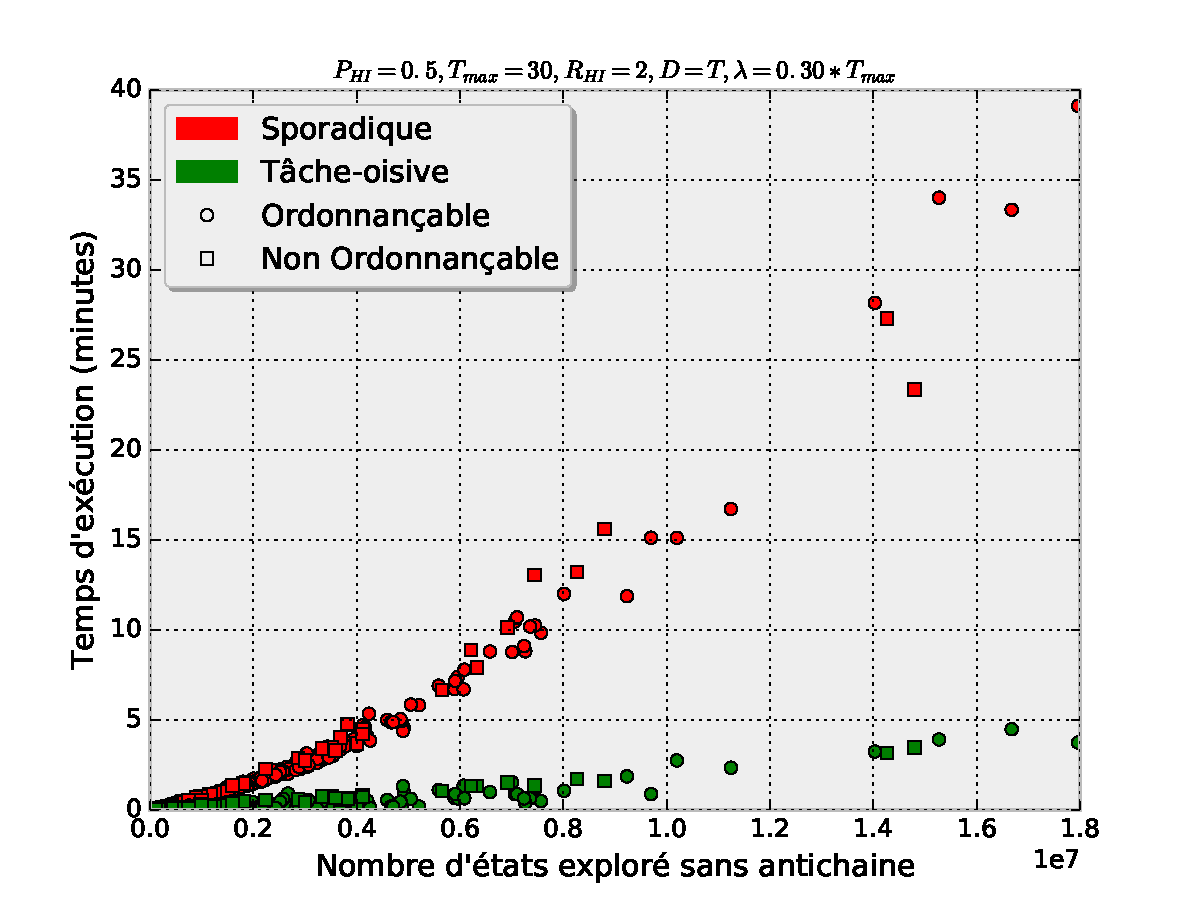
\includegraphics[width=\textwidth]{./results/timeSpoIdle.pdf}
\caption{Analyse de la performance de la relation de simulation}
\end{figure}

\begin{figure}[h]
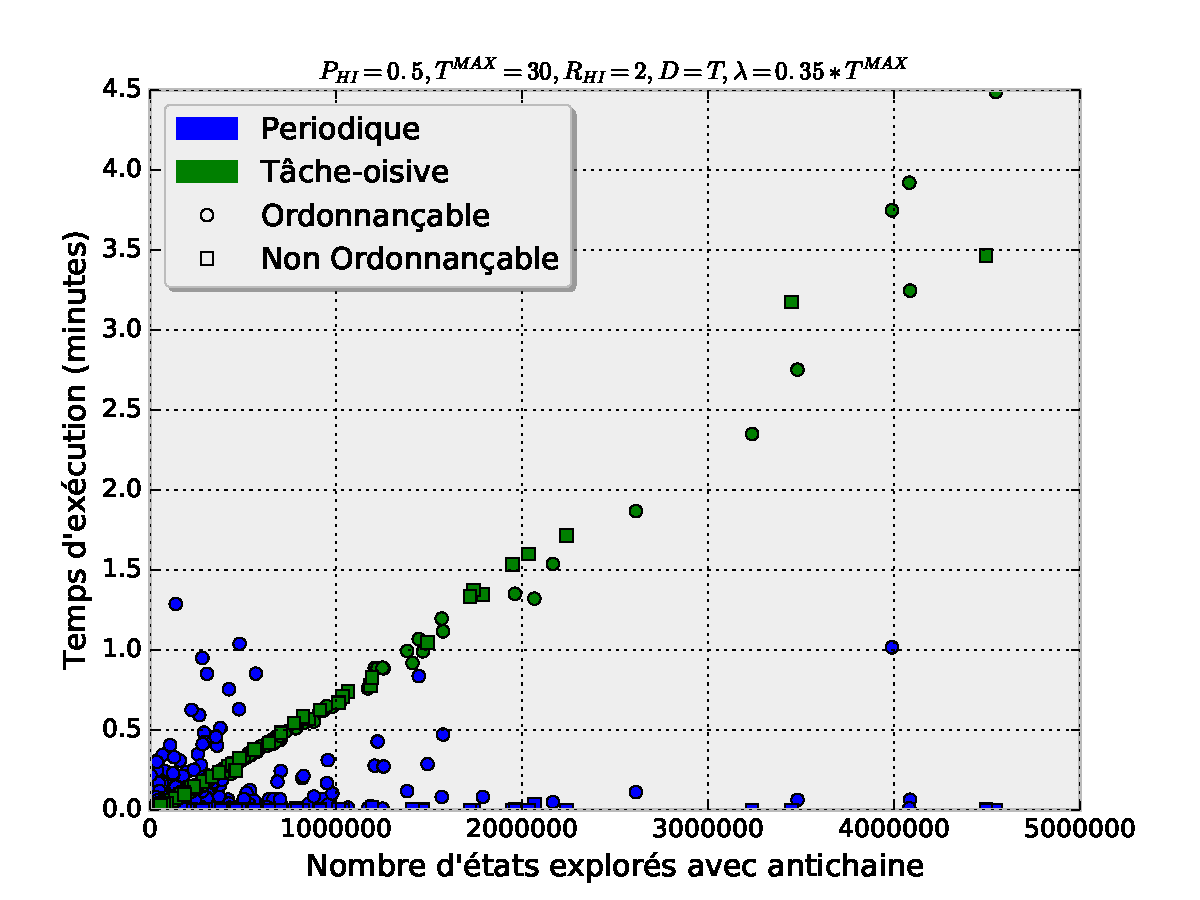
\includegraphics[width=\textwidth]{./results/timePerIdle.pdf}
\caption{Analyse de la performance de la relation de simulation}
\end{figure}

\begin{figure}[h]
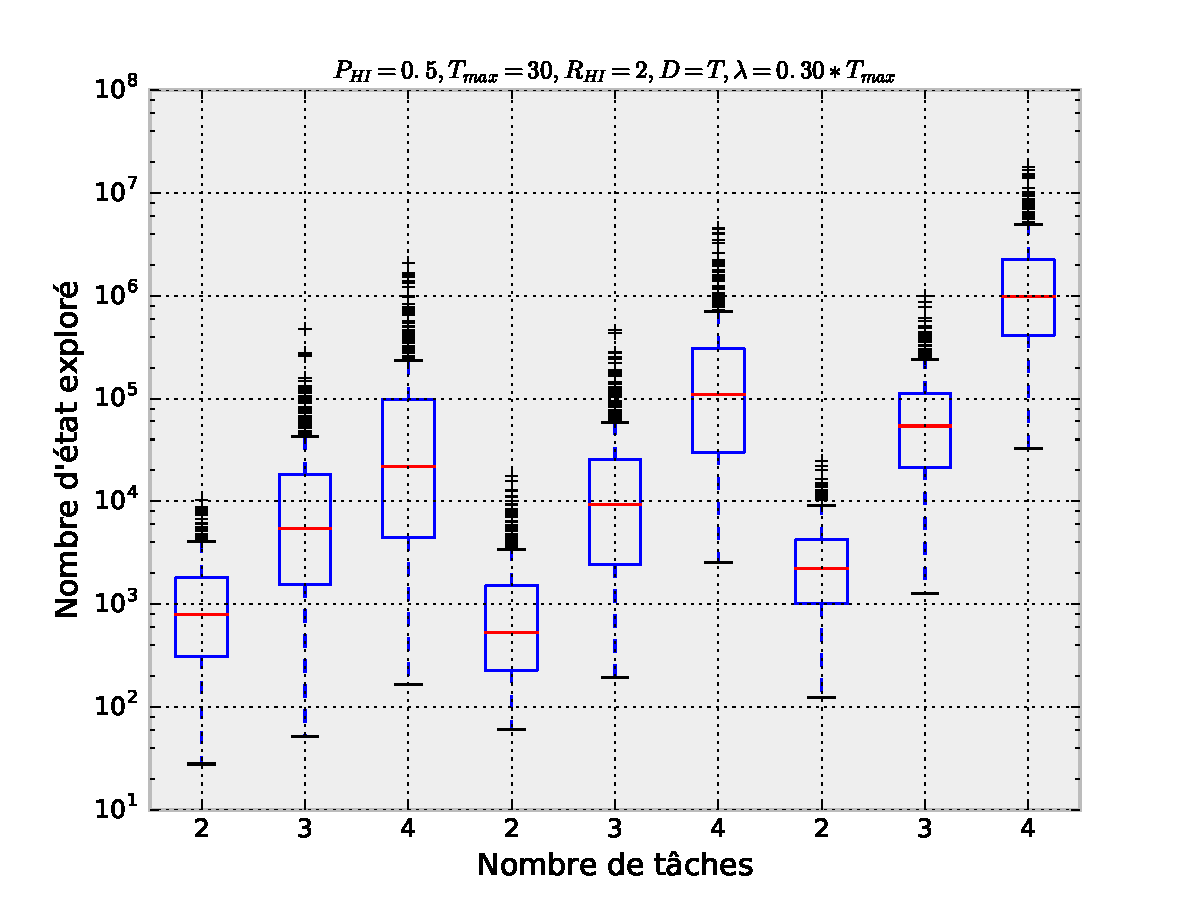
\includegraphics[width=\textwidth]{./results/taskvssize.pdf}
\caption{Taille de l'automate en fonction du nombre de tâches}
\end{figure}

\section{Analyse de l'ordonnancement}

\begin{figure}[h]
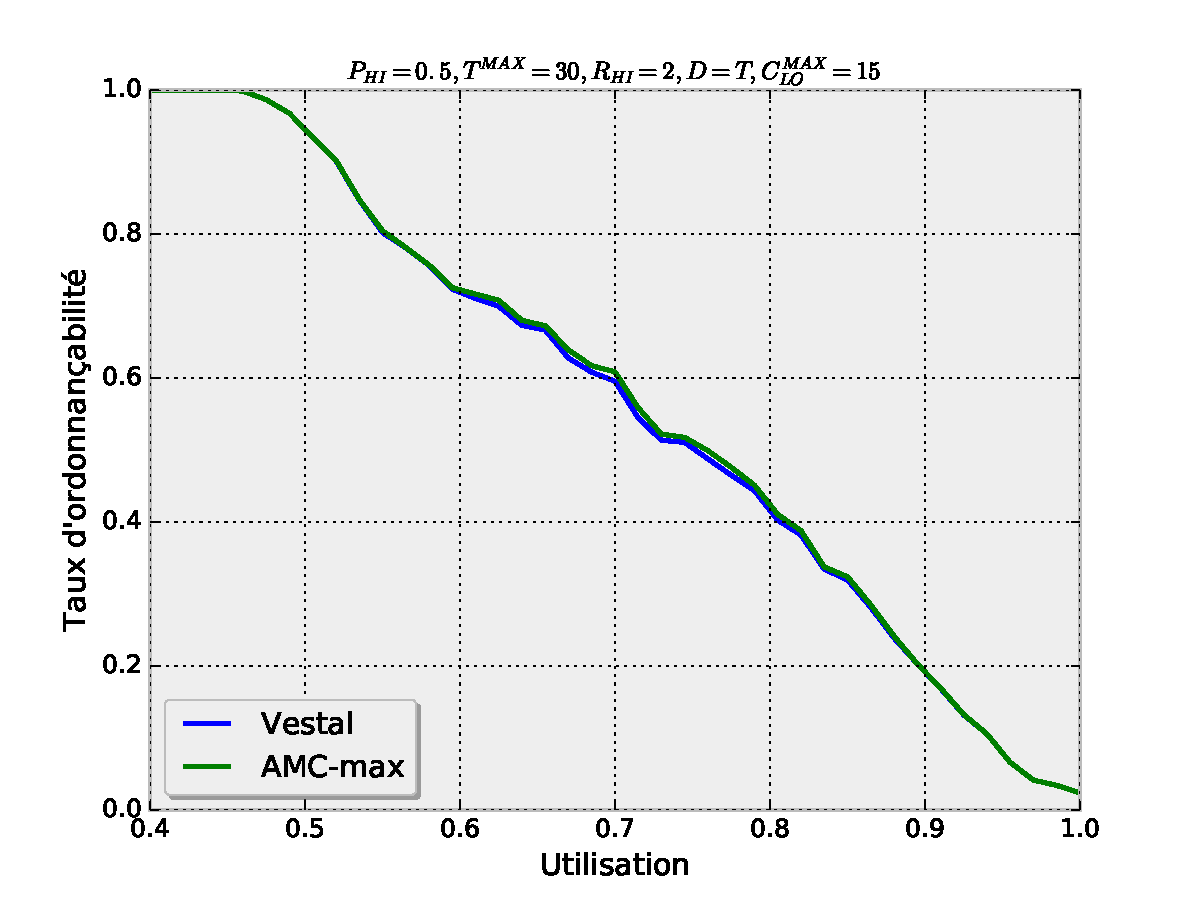
\includegraphics[width=\textwidth]{./results/perfAMCVestal.pdf}
\caption{Ordonnançabilité de Vestal et AMC-max}
\end{figure}

\begin{figure}[h]
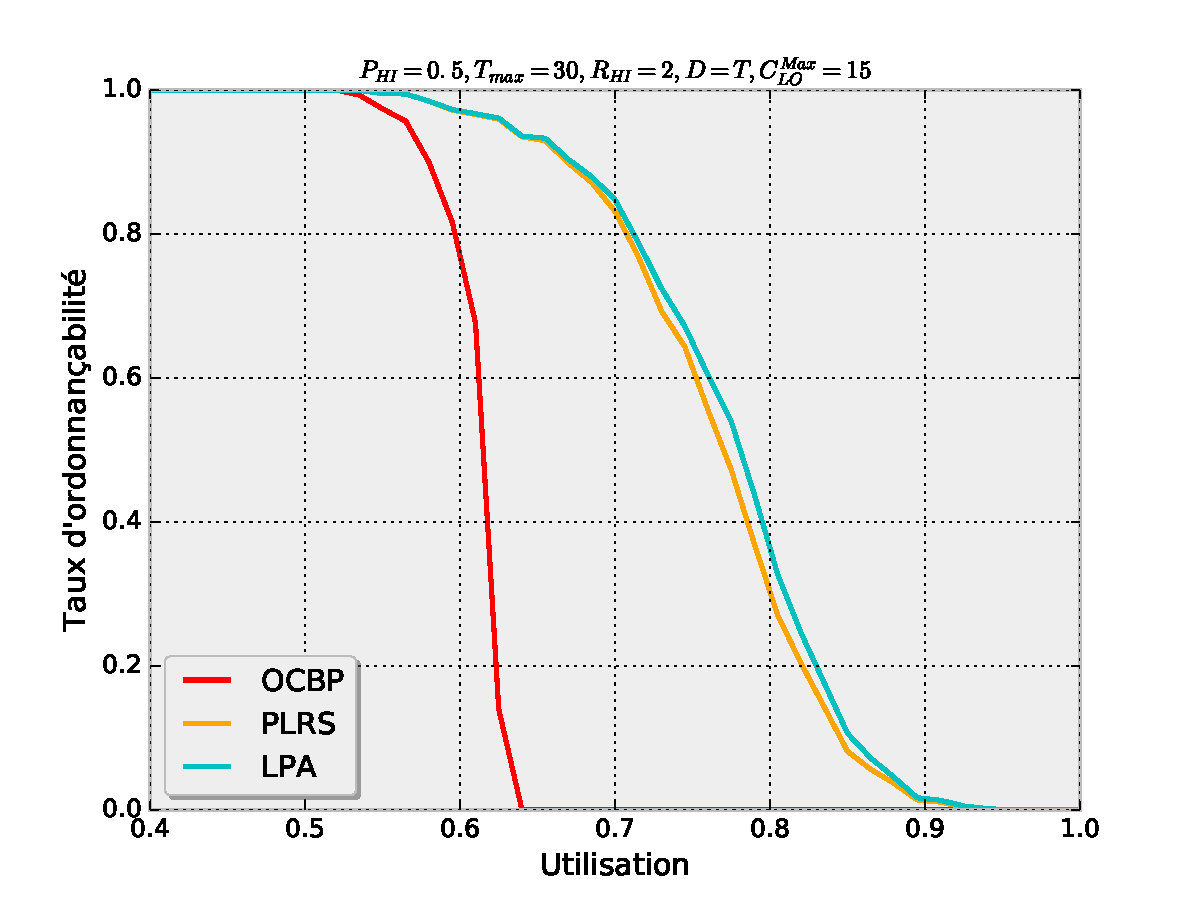
\includegraphics[width=\textwidth]{./results/perfOCBPetc.pdf}
\caption{Ordonnançabilité de OCBP et extensions}
\end{figure}

\begin{figure}[h]
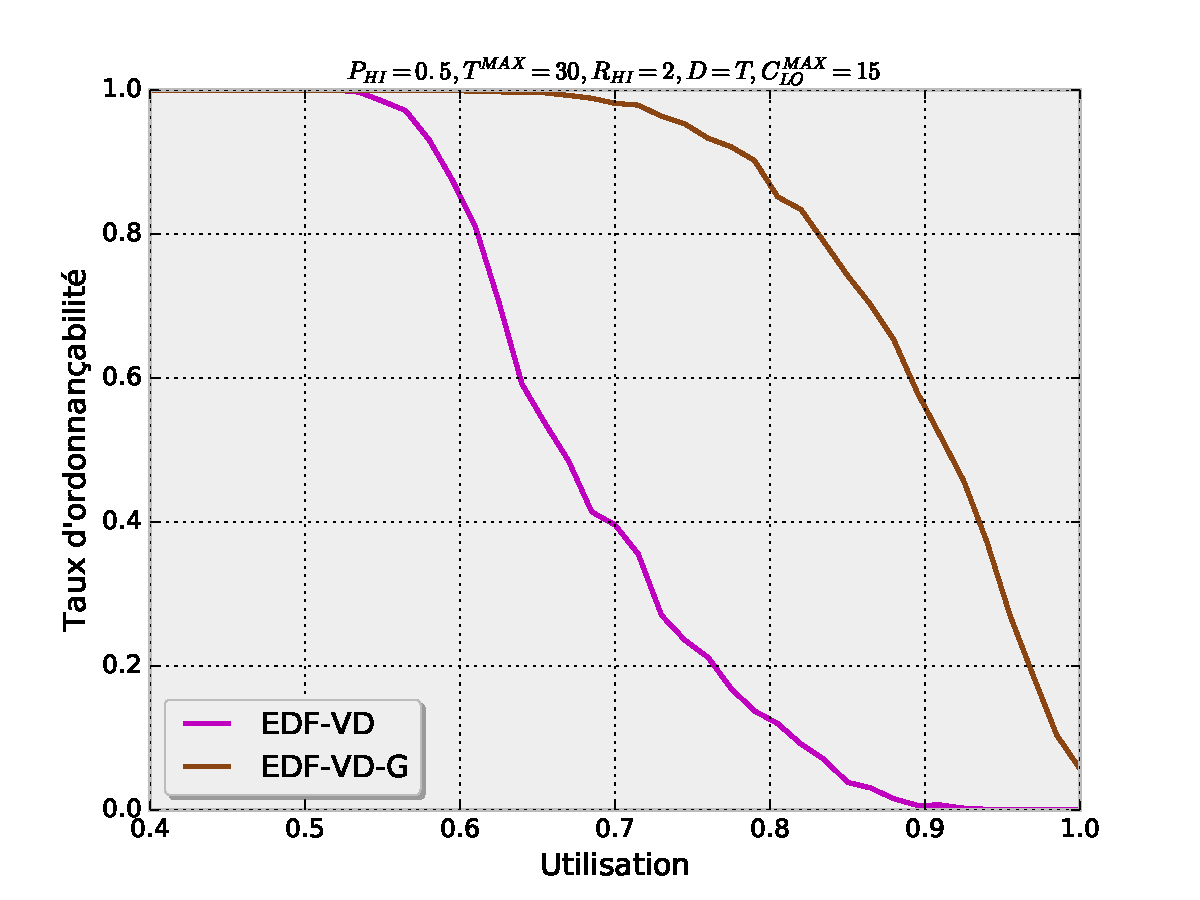
\includegraphics[width=\textwidth]{./results/perfEDFVD.pdf}
\caption{Ordonnançabilité de EDF-VD}
\end{figure}

\begin{figure}[h]
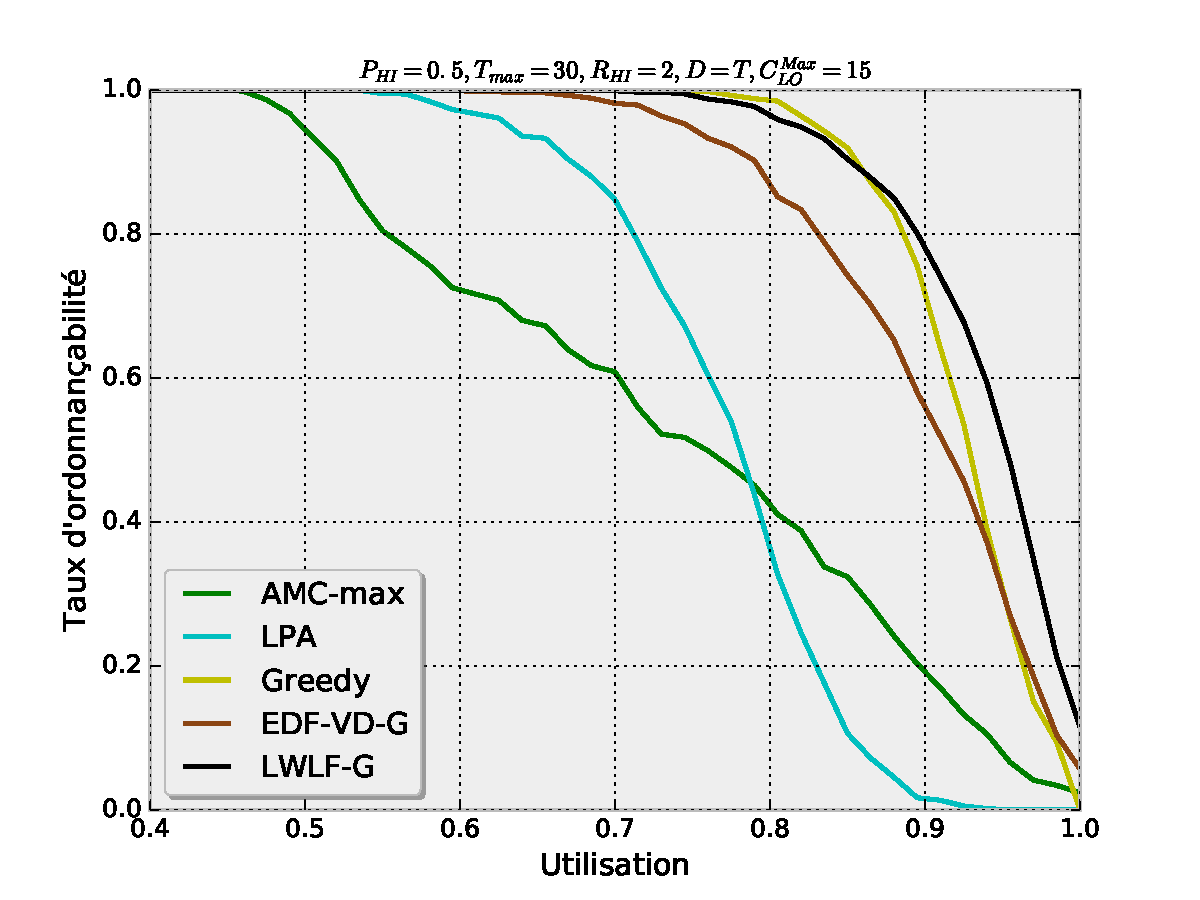
\includegraphics[width=\textwidth]{./results/perfComp.pdf}
\caption{Comparaison des algorithmes}
\end{figure}



\chapter{Conclusion}



%\nocite{*}
\bibliographystyle{unsrt}
%\bibliographystyle{plain}
\bibliography{./reference/bibliography}
\end{document}

